%%%%%%%%%%%%%%%%%%%%%%%%%%%%%%%%%%%%%%%%%%%%%%%%%%%%%%%%%%%%%%%%%%%%%
%
%  This is a sample LaTeX input file for your contribution to
%  the MC2013 conference. Modified by R.C. Martineau at INL from A.
%  Sood at LANL, from J. Wagner ORNL who obtained the original class
%  file by Jim Warsa, LANL, 16 July 2002}
%
%  Please use it as a template for your full paper
%    Accompanying/related file(s) include:
%       1. Document class/format file: mc2013.cls
%       2. Sample Postscript Figure:   figure.eps
%       3. A PDF file showing the desired appearance: template.pdf
%    Direct questions about these files to: richard.martinea@inl.gov
%
%    Notes:
%      (1) You can use the "dvips" utility to convert .dvi
%          files to PostScript.  Then, use either Acrobat
%          Distiller or "ps2pdf" to convert to PDF format.
%      (2) Different versions of LaTeX have been observed to
%          shift the page down, causing improper margins.
%          If this occurs, adjust the "topmargin" value in the
%          mc2013.cls file to achieve the proper margins.
%
%%%%%%%%%%%%%%%%%%%%%%%%%%%%%%%%%%%%%%%%%%%%%%%%%%%%%%%%%%%%%%%%%%%%%


%%%%%%%%%%%%%%%%%%%%%%%%%%%%%%%%%%%%%%%%%%%%%%%%%%%%%%%%%%%%%%%%%%%%%
\documentclass{anstopical-class/ansconf}
%
%  various packages that you may wish to activate for usage
\usepackage{graphicx}
\usepackage{tabls}
\usepackage{multirow}
%
% my packages
\usepackage{amsmath} % math stuff
\usepackage{amssymb} % more math stuff
\usepackage{siunitx} % units and stuff
\sisetup{detect-weight=true, detect-family=true} % makes siunitx follow font formatting like bold, italic, etc.
\usepackage{cancel} % cancel stuff in eqns
\usepackage{isotope} % makes isotopes look pretty
\usepackage{listings} % makes code look pretty
\usepackage[dvipsnames,table]{xcolor} % colors
\usepackage{xspace} % space
\usepackage{booktabs} % table stuff
\usepackage{setspace} % more space
\usepackage{subcaption} % subfigure stuff
\usepackage{svg} % svg format figure stuff
\usepackage{hyperref} % makes refs good
\usepackage[final]{varioref} % makes refs even gooder
\usepackage{cleveref} % makes refs gooder
% adds oxford comma to cleveref
\newcommand{\creflastconjunction}{, and\nobreakspace}
\usepackage{lipsum} % lorem ipsum filler

% si units stuff
\DeclareSIUnit\year{yr}
\DeclareSIUnit\hour{hr}
\DeclareSIUnit\amp{A}

% check and x marks
\usepackage{pifont}% http://ctan.org/pkg/pifont
\newcommand{\cmark}{\textcolor{Green}{\ding{51}}}%
\newcommand{\xmark}{\textcolor{Red}{\ding{55}}}%
%
% Insert authors' names and short version of title in lines below
%
%\authorHead{Authors' names, use et al. if more than 3}
%\shortTitle{Short version of title as entered by author on web %page}

%\confTitle{19$^{th}$ International Conference on Nuclear Reactor %Thermal Hydraulics (NURETH-19)}
%\confLocation{Brussels, Belgium, August 29 -- September 3, 2021}

%Header and Page numbers

\usepackage{fancyhdr,graphicx,lastpage}% http://ctan.org/pkg/{fancyhdr,graphicx,lastpage}
\fancypagestyle{plain}{
\fancyhf{}
\fancyhead[L]{\begin{tabular}{ll}
\multirow{2}{*}{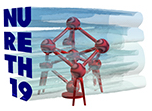
\includegraphics[scale=0.28]{anstopical-class/NURETH-19.png}} & \fontsize{9}{9}\selectfont {\setstretch{0.1}}The 19th International Topical Meeting on Nuclear Reactor Thermal Hydraulics (NURETH-19) Log nr.: 19001 \\
& \fontsize{9}{9}\selectfont Brussels, Belgium, March 6 - 11, 2022 \\
\end{tabular}} 
\fancyfoot[C]{\thepage}% Right footer
}



%%%%%%%%%%%%%%%%%%%%%%%%%%%%%%%%%%%%%%%%%%%%%%%%%%%%%%%%%%%%%%%%%%%%%
%
%   BEGIN DOCUMENT
%
%%%%%%%%%%%%%%%%%%%%%%%%%%%%%%%%%%%%%%%%%%%%%%%%%%%%%%%%%%%%%%%%%%%%%





\pagestyle{plain}% Set page style to plain.

\begin{document}

\title{EXPERIMENTS ON THE HELIUM-3 NEGATIVE REACTIVITY INSERTION (HENRI) PROTOTYPE AND FAST OPENING VALVE}

\author{A. Warren}
\author{A. Camargo}
\author{G. Mignot}
\author{W. Marcum}
\affil{School of Nuclear Science and Engineering \\
  Oregon State University, Corvallis, OR 97331 \\
  warrenau@oregonstate.edu; camargoa@oregonstate.edu}

%\author{Double space and list Author C}
%\affil{
%  Department of Nuclear Engineering \\
%  Name of University \\
%  Address \\
%  C@name.univ.edu
%}

\maketitle

\begin{abstract}
The restart of the TRansient REactor Test (TREAT) facility combined with the Resumption of Transient Testing Program (RTTP) has generated an increased interest in mimicking Reactivity Initiated  Accident (RIA) events conditions for Light Water Reactor within TREAT itself. One of the engineering challenges for this task is to increase the energy deposition rate on the tested fuel element by shortening the width of the  power  pulse  from  its  current  89  milliseconds down  to  40 milliseconds. To overcome  this  challenge, Idaho National Laboratory (INL) proposed a design, consisting of rapidly pressurizing a specially designed hollow control rod with Helium-3. The insertion of negative reactivity in the form of Helium-3, a strong neutron  absorber,  must  be  well  predicted and repeatable.  In  this  prospect,  an  out-of-pile  prototype,  the Helium  Negative  Reactivity  Insertion  (HENRI) facility, has been designed  and  built  at  Oregon  State University (OSU) to  assess  the  feasibility,  the  repeatability, and  the control of such process. Tests performed with rupture disks provided characterization of the physics of the system, however the system requires a more repeatable and precise method of gas injection. To meet this need, a valve has been designed and tested using a pneumatic piston which can open rapidly and repeatedly for precise control of the system. These tests characterized the valve performance and provided confidence in the operation of the system, both of which are critical to understand and control the Helium-3 density evolution in the core.

\raggedleft
\textbf{KEYWORDS}\\
TREAT, Helium-3, Control Rod, Pulse, Valve
\end{abstract}


%\raggedright

%%%%%%%%%%%%%%%%%%%%%%%%%%%%%%%%%%%%%%%%%%%%%%%%%%%%%%%%%%%%%%%%%%%%%%%
%%%%%%%%%%%%%%%%%%%%%%%%%%% INTRODUCTION %%%%%%%%%%%%%%%%%%%%%%%%%%%%%%
%%%%%%%%%%%%%%%%%%%%%%%%%%%%%%%%%%%%%%%%%%%%%%%%%%%%%%%%%%%%%%%%%%%%%%%
% probably similar to previous HENRI NURETH intro
% motivations for TREAT RIA testing / HENRI project
% discuss the need for the fast opening piston valve -- maybe needs a different section?
\section{Introduction} \label{s:intro}

% start with introduction / motivations of entire HENRI project
The Transient Reactor Test (TREAT) facility, located at the Materials and Fuels Complex at Idaho National Laboratory (INL), is a research reactor with the primary purpose of testing fuels under transient conditions and supporting the development of accident-tolerant fuel \cite{CINBIZ2017}. The reactor can shape these transients using control rods and the negative reactivity temperature feedback, with a maximum energy deposition of \SI{2500}{\mega\joule} \cite{Holschuh2019}. Currently, with this energy deposition limit, the pulse full-width at half-maximum (FWHM) TREAT is capable of generating is around \SI{100}{\milli\second} \cite{Holschuh2019}. This pulse width is outside of the range for a Light Water Reactor (LWR) Reactivity Initiated Accident (RIA) of 30 to \SI{60}{\milli\second} \cite{NEA2010}. A limited number of research reactors are able to produce transient conditions representative of LWRs. \Cref{fig:trans comp} presents a comparison of transient conditions that can be produced by contemporary reactors. There are not any reactors that are able to reproduce the conditions (FWHM and maximum power) of a LWR RIA. The Power Burst Facility (PBF) is the closest to matching the conditions of an LWR RIA, however it has been decommissioned and cannot be used. Using its control rods, TREAT can decrease its transient FWHM down to \SI{89}{\milli\second} \cite{NEA2010}, shown as a red dashed line in \Cref{fig:trans comp}. A further reduction in FWHM would bring TREAT near BWR conditions.



% transient reactor comparison plot -- ripped from source paper by Bess -- look for the one Mignot used in the old nureth paper
\begin{figure}[htbp]
    \vspace{16pt}
    \centering
    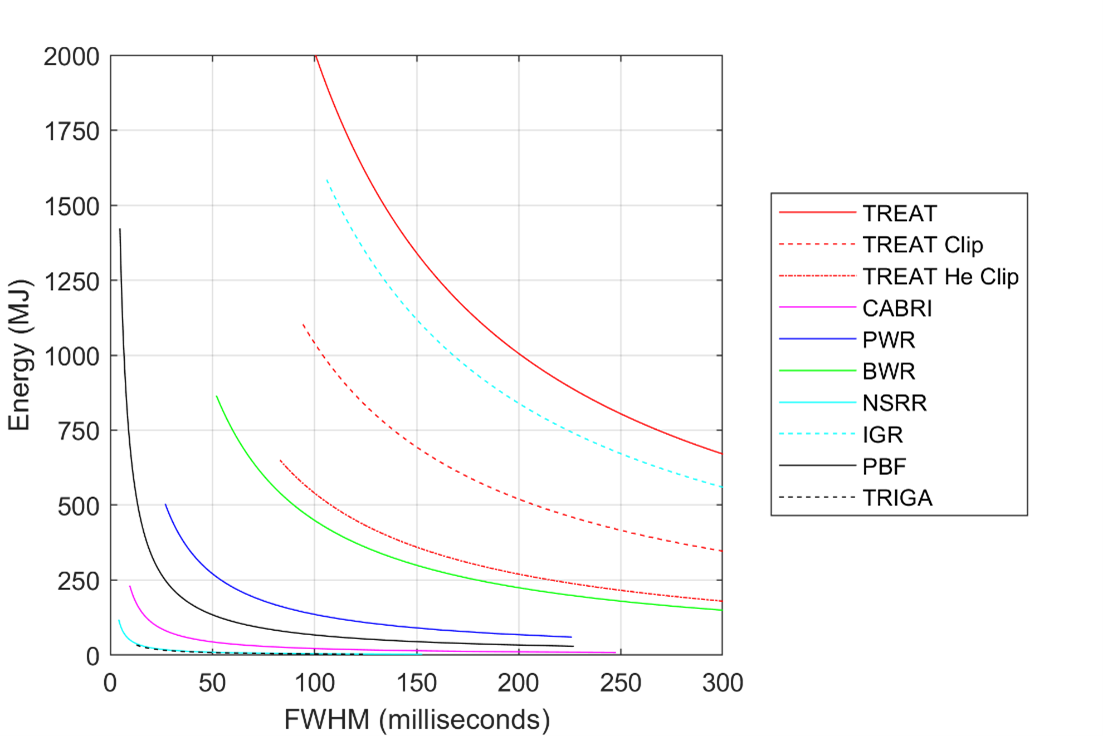
\includegraphics[width=0.75\textwidth]{intro/plots/ReactorTransientComp_Kevin.png}
    \caption{Comparison of contemporary reactor transient conditions \cite{BESS2019}.}
    \label{fig:trans comp}
    \vspace{16pt}
\end{figure}


Crawford \cite{Crawford1998} suggested the use of helium-3, a strong neutron absorber gas, for clipping a high-power pulse in TREAT. Such a system would be capable of inserting a negative reactivity of -5\% $\Delta k/k$ without the use of control rods. The original calculation results in a FWHM reduced to 40-\SI{60}{\milli\second} for a total energy deposition of \SI{1600}{\mega\joule}, well below the \SI{2500}{\mega\joule} limit, and the peak power was estimated to be \SI{20000}{\mega\watt}. This pulse is more representative of the postulated LWR RIA and is shown as a red dotted line in \Cref{fig:trans comp}.

Helium-3 has been used for a similar purpose at the CABRI reactor in Cadarache, France. At CABRI, helium-3 is pressurized in 4 tubes in the core, then to initiate a transient, the helium-3 is rapidly depressurized from the core (negative reactivity removal). This depressurization is precisely controlled using multiple valves to produce the desired pulse width and power for the transient \cite{Clamens2016,Clamens2018,Clamens2018b}. In TREAT, this process will be reversed by rapidly pressurizing tubes in the core with helium-3 to shut down a transient (negative reactivity insertion). CABRI has been updated and is currently used under the OECD/NEA CABRI International Project (CIP).

Initial calculations for the TREAT facility showed that a helium-3 pressure of \SI{1.72}{\mega\pascal} (\SI{250}{psi}) in a cartridge volume of \SI{1167}{\centi\meter^3} would be sufficient to reach the desired negative reactivity of -5\% $\Delta k/k$. This pressure corresponds to an atomic density of \SI{3.35e20}{atoms\per\centi\meter^3}. For a pulse to be clipped properly, it is estimated that the helium-3 must be injected in \SI{5}{\milli\second} \cite{BESS2019}. Oregon State University (OSU) was tasked to model, design, and test an out-of-pile prototype cartridge to assess the feasibility and repeatability of the physical process; and identify and solve any engineering issues associated with the device. The experimental Helium-3 Negative Reactivity Insertion (HENRI) facility was designed and built at OSU. Testing was performed to determine the feasibility and repeatability of the gas injection, with positive results \cite{HeNURETH}. This paper presents updates to the HENRI facility, as well as continued work in the experimental campaign, specifically focusing on the development and testing of a bespoke fast-opening valve for the facility.



% describe the need for a new fast-opening valve -- should this be its own section?
\subsection{Need for a Fast-opening Valve} \label{s:need for valve}

The previous work on HENRI at OSU \cite{HeNURETH} used rupture disks to characterize the system and its physics. Rupture disks provided an almost instantaneous opening, which allowed for the gas physics to be isolated and compared against CFD models \cite{CFDNureth}. The rupture disks, however, have major drawbacks for use in the HENRI system for TREAT. Firstly, the rupture disks must be changed after each use, which would mean taking the HENRI system out of the TREAT reactor and dealing with the radiation of the system before changing the rupture disk and reinstalling the system in the reactor. This process adds danger and complexity, on top of the time, to a system intended to be utilized heavily during RIA testing campaigns. Secondly, the rupture disks do not rupture in a predictable manner. There is tolerance in the manufacture of rupture disks that causes the disks to rupture at slightly different pressures, which is not ideal when the system needs to be precisely timed with the peak of a transient. These problems with the rupture disk have lead OSU to investigate a more permanent valve option. This valve must be reusable, precise, fast-opening, and durable. The valve must also fit into the physical space constraints of the HENRI system, which includes its power or actuation method, and not contaminate the helium-3 used in the system.





\clearpage
%%%%%%%%%%%%%%%%%%%%%%%%%%%%%%%%%%%%%%%%%%%%%%%%%%%%%%%%%%%%%%%%%%%%%%%
%%%%%%%%%%%%%%%%%%%%%%%%%%%%%% DESIGN %%%%%%%%%%%%%%%%%%%%%%%%%%%%%%%%%
%%%%%%%%%%%%%%%%%%%%%%%%%%%%%%%%%%%%%%%%%%%%%%%%%%%%%%%%%%%%%%%%%%%%%%%
% discuss design requirements of fast opening valve -- why piston valve; why does burst disk not work
% discuss design iterations of piston valve -- first mount / metal-metal seal, then improved mount, and o-ring on plug
\section{Fast-Opening Valve Design} \label{s:design}
% talk about design requirements
% discuss the initial piston valve design -- what was it, how well did it work, why did it not work
A valve for use in HENRI must be: fast-opening, predictable, reliable, reusable, fit in the physical confines of the HENRI system, and not contaminate or disrupt the helium-3. 
To meet these requirements, a pneumatic piston valve was designed and a prototype was built at OSU. The valve utilizes a pneumatic piston, which uses helium as its working fluid, to press a metal `plug' against a machined flange surface to seal the high pressure driver tank from the evacuated test section. The piston is mounted to the flange and is fed helium via an external manifold that is connected through the flange using tube fittings. The plug is held closed by the piston pressure in the bottom chamber, as well as the pressure in the driver tank. When the piston is desired to be opened, the helium is vented from the bottom chamber, then the top chamber is pressurized rapidly to actuate the piston and remove the plug from the exit of the driver tank. Using the helium of the HENRI system as the working gas for the piston provides some advantages: firstly, using only helium in the system reduces the chances of contamination, which is vitally important for a system that will be full of rare helium-3 gas, both for neutronics and for economics, and secondly, using high pressure gas allows for rapid actuation of the piston, which will compensate for the slower actuation when compared to the rupture disk.

% obviously put a drawing and/or picture here of the og design -- also include a picture of the whole HENRI assembly with labels, so this all makes sense

% should we talk about opening speed characterization? if so, we need plots / tables of results and maybe some pics of the set up

The first plug design was made with various materials, including aluminum, stainless steel, and a cobalt alloy, seen in \Cref{fig:metal plugs}. This plug is a simple design with a \SI{45}{\degree} cone that directly contacts the matching machined surface of the flange. A special coating was also tried on an aluminum plug[DO WE HAVE THE COATING INFO?] to improve the sealing ability of the plug on the flange. The initial mount design for the piston was made of a plate mounted to the piston body and three legs holding the plate onto the flange. The three-legged design allowed for easy routing of tubing for operating the piston, but also allowed for some movement of the mount when the piston was fully extended. This movement caused asymmetric wear on the plug, as seen in \Cref{fig:metal plugs}, leading to failure of the seal. Potentially due to this wear, the slow flow through the manifold, or the nature of metal-to-metal seals, a slight leak was observed from the driver tank into the test section before the piston valve opened fully [REF to plot here?].
% need pics of all 1st gen plugs compared to each other w/ wear
\begin{figure}[htbp]
    \vspace{16pt}
    \centering
    %\includegraphics{}
    \caption{Plugs used for metal-to-metal seal. Clockwise, starting from the top left: [plug materials in order]}
    \label{fig:metal plugs}
    \vspace{16pt}
\end{figure}

% discuss metal-to-metal seal problems at low pressure
An additional requirement for the HENRI system from the TREAT team is that the valve can operate at low pressures in the driver tank, to broaden the range of experiments TREAT can use HENRI for. The valve design uses both the pressure in the driver tank and the pressure in the piston to hold the plug closed, but if the pressure in either is low enough, there may not be enough sealing force to keep the helium from leaking. It was found with the metal-to-metal seal that it was difficult to keep the seal with a driver tank pressure less than \SI{500}{psia}[NEED TO CHECK, maybe add figure here, or ref results]. Low pressure sealing was difficult for this design, even with fresh plugs that had not been worn by the metal-to-metal contact.

% discuss design improvements in second iteration in both the mount and the o-ring
\subsection{Design Iteration} \label{s:iteration}
While the first plug and mount design proved the concept of a piston valve will work for the HENRI system, the seal durability was low and the piston opening was not as smooth or as fast as desired. To improve the valve, a new plug was designed using an o-ring to improve the sealing ability, and a new mount was designed to provide a more uniform and sturdy hold on the piston. The new assembly can be seen in \Cref{fig:piston assembly}. The new plug still uses a \SI{45}{\degree} slope to mate to the existing flange, but it does not go to a point like the previous design. It has a dovetail groove machined into it, as seen in \Cref{fig:Dovetail Groove}, to hold the o-ring in place such that the o-ring presses into the machined surface of the flange to strongly seal the driver tank from the test section. Two types of o-ring materials have been tested: an FFKM o-ring manufactured by Marko Rubber and a nitrile o-ring manufactured by Parker. The new mount was designed to work with the existing flange, so it uses the same bolt holes and needs to align the piston with the same sealing surface. The mount utilizes three aluminum pieces: a circular plate mounted to the bottom of the piston, a circular plate to hold the mount on the flange, and a cylindrical support holding the two plates together and keeping the piston at the correct distance from the sealing surface. The cylindrical support has slots machined into to allow for gas flow, tube fitting connections on the piston, and access to the bolts that mount the assembly to the flange.

% maybe include a table with serial numbers for o-rings?

% need images / diagrams of 2nd gen plug and mount system
%
\begin{figure}[htbp]
    \vspace{16pt}
    \centering
    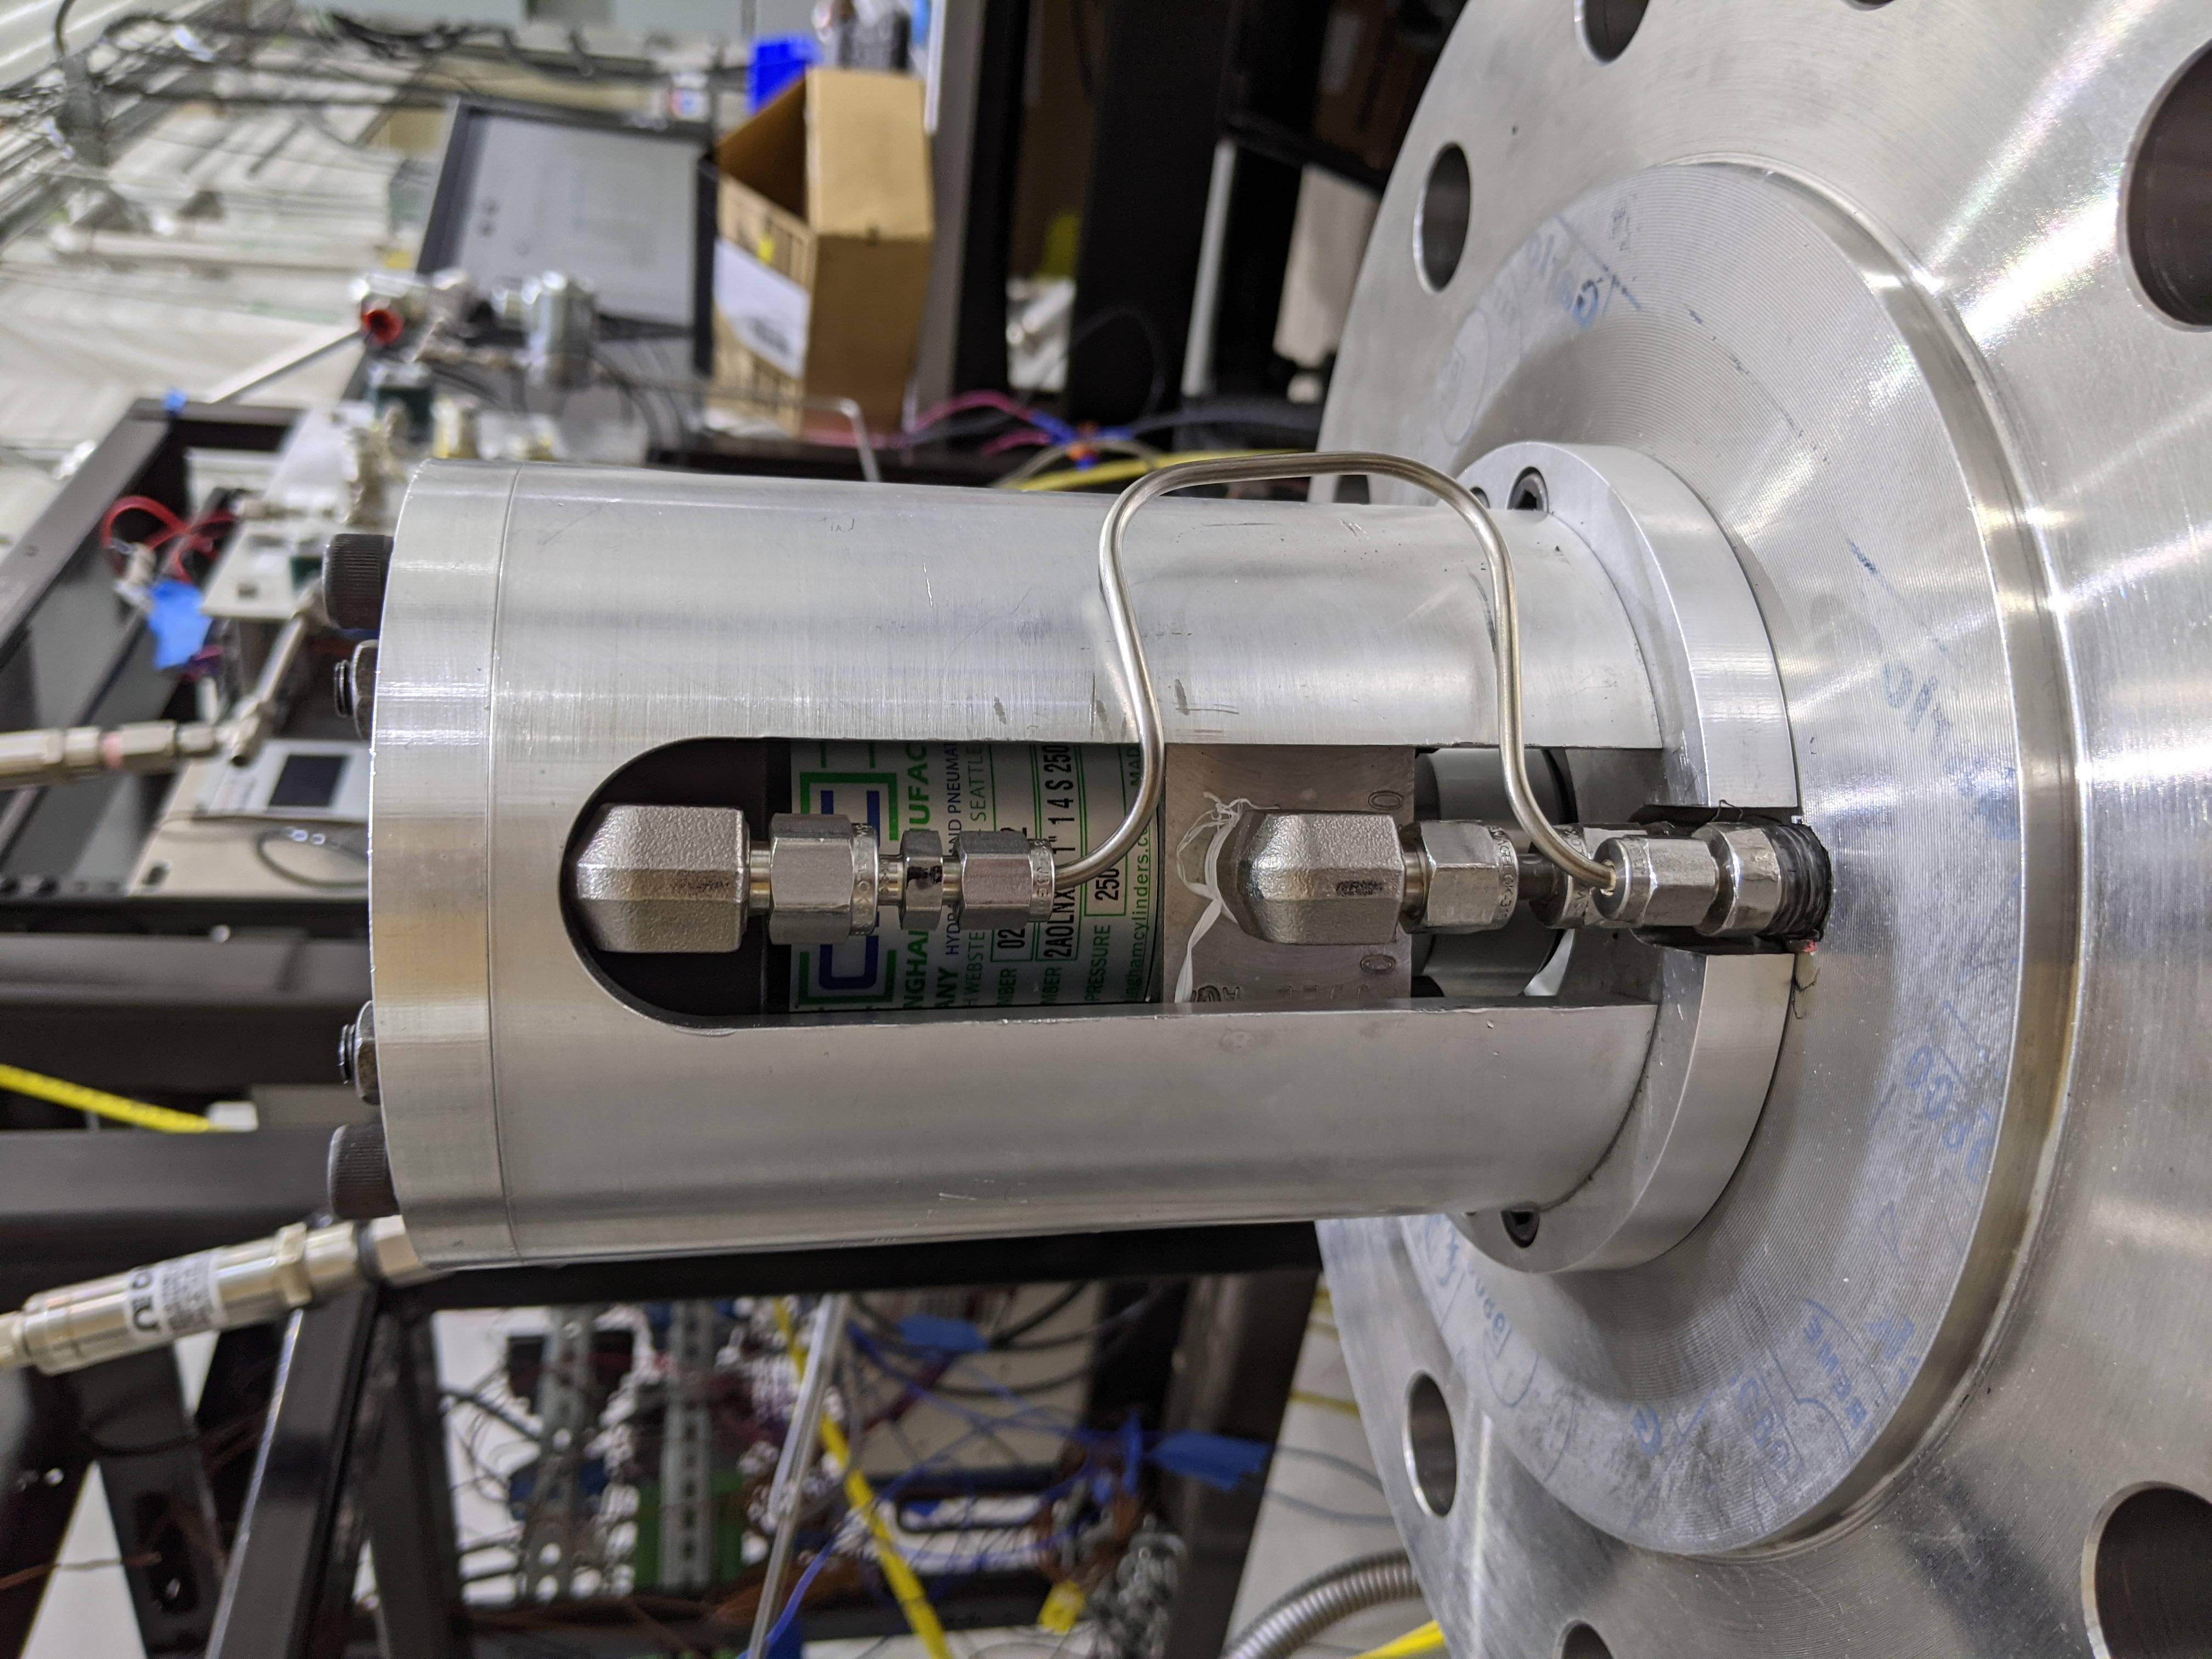
\includegraphics[height=2.625in, width=3.5in,angle=270]{experiment/photos/Piston_Assembly.jpg} % for some reason, overleaf rotates this and it looks correct in overleaf, but it is not in a downloaded pdf -- this needs to be rotated to be correct in pdf -- you can look at it by downloading the pdf or changing the viewer to 'native' in the menu, instead of 'built-in'
    \caption{Piston assembled with second generation mount on flange.}
    \label{fig:piston assembly}
    \vspace{16pt}
\end{figure}
%


% dovetail

\begin{figure}[htbp]
    \vspace{16pt}
    \centering
    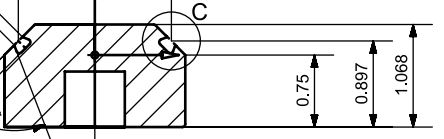
\includegraphics[width=4.032in]{design/photos/dovetail.JPG}
    \caption{Cutaway view of the second generation plug, with dovetail groove for o-ring. Measurements are in inches.}
    \label{fig:Dovetail Groove}
    \vspace{16pt}
\end{figure}




% discuss future design improvements that have not yet been implemented -- new driver tank, proposed improvements to flange / piston pressure lines, etc.
\subsection{Future Improvements} \label{s:improvements}
Going forward, there is still work to be completed in the design process. Firstly, the HENRI prototype will need to be fitted with a driver tank that is more representative of the final HENRI system. This driver tank has been designed and fabricated, however the flange has not been machined to accept the piston valve. Also, the o-ring durability must continue to be tested, as o-rings have broken during testing at OSU, as seen in \Cref{fig:broken oring piston,fig:broken oring 2}. The exact cause of the o-ring failure has yet to be determined, but a testing campaign is underway to investigate the problem further.

% o-ring failure pics -- do we want these here? they take up a lot of space and we might not want to talk too much about the o-ring failures. Maybe just have one of the two figs?

\begin{figure}[htbp]
    \vspace{16pt}
    \centering
    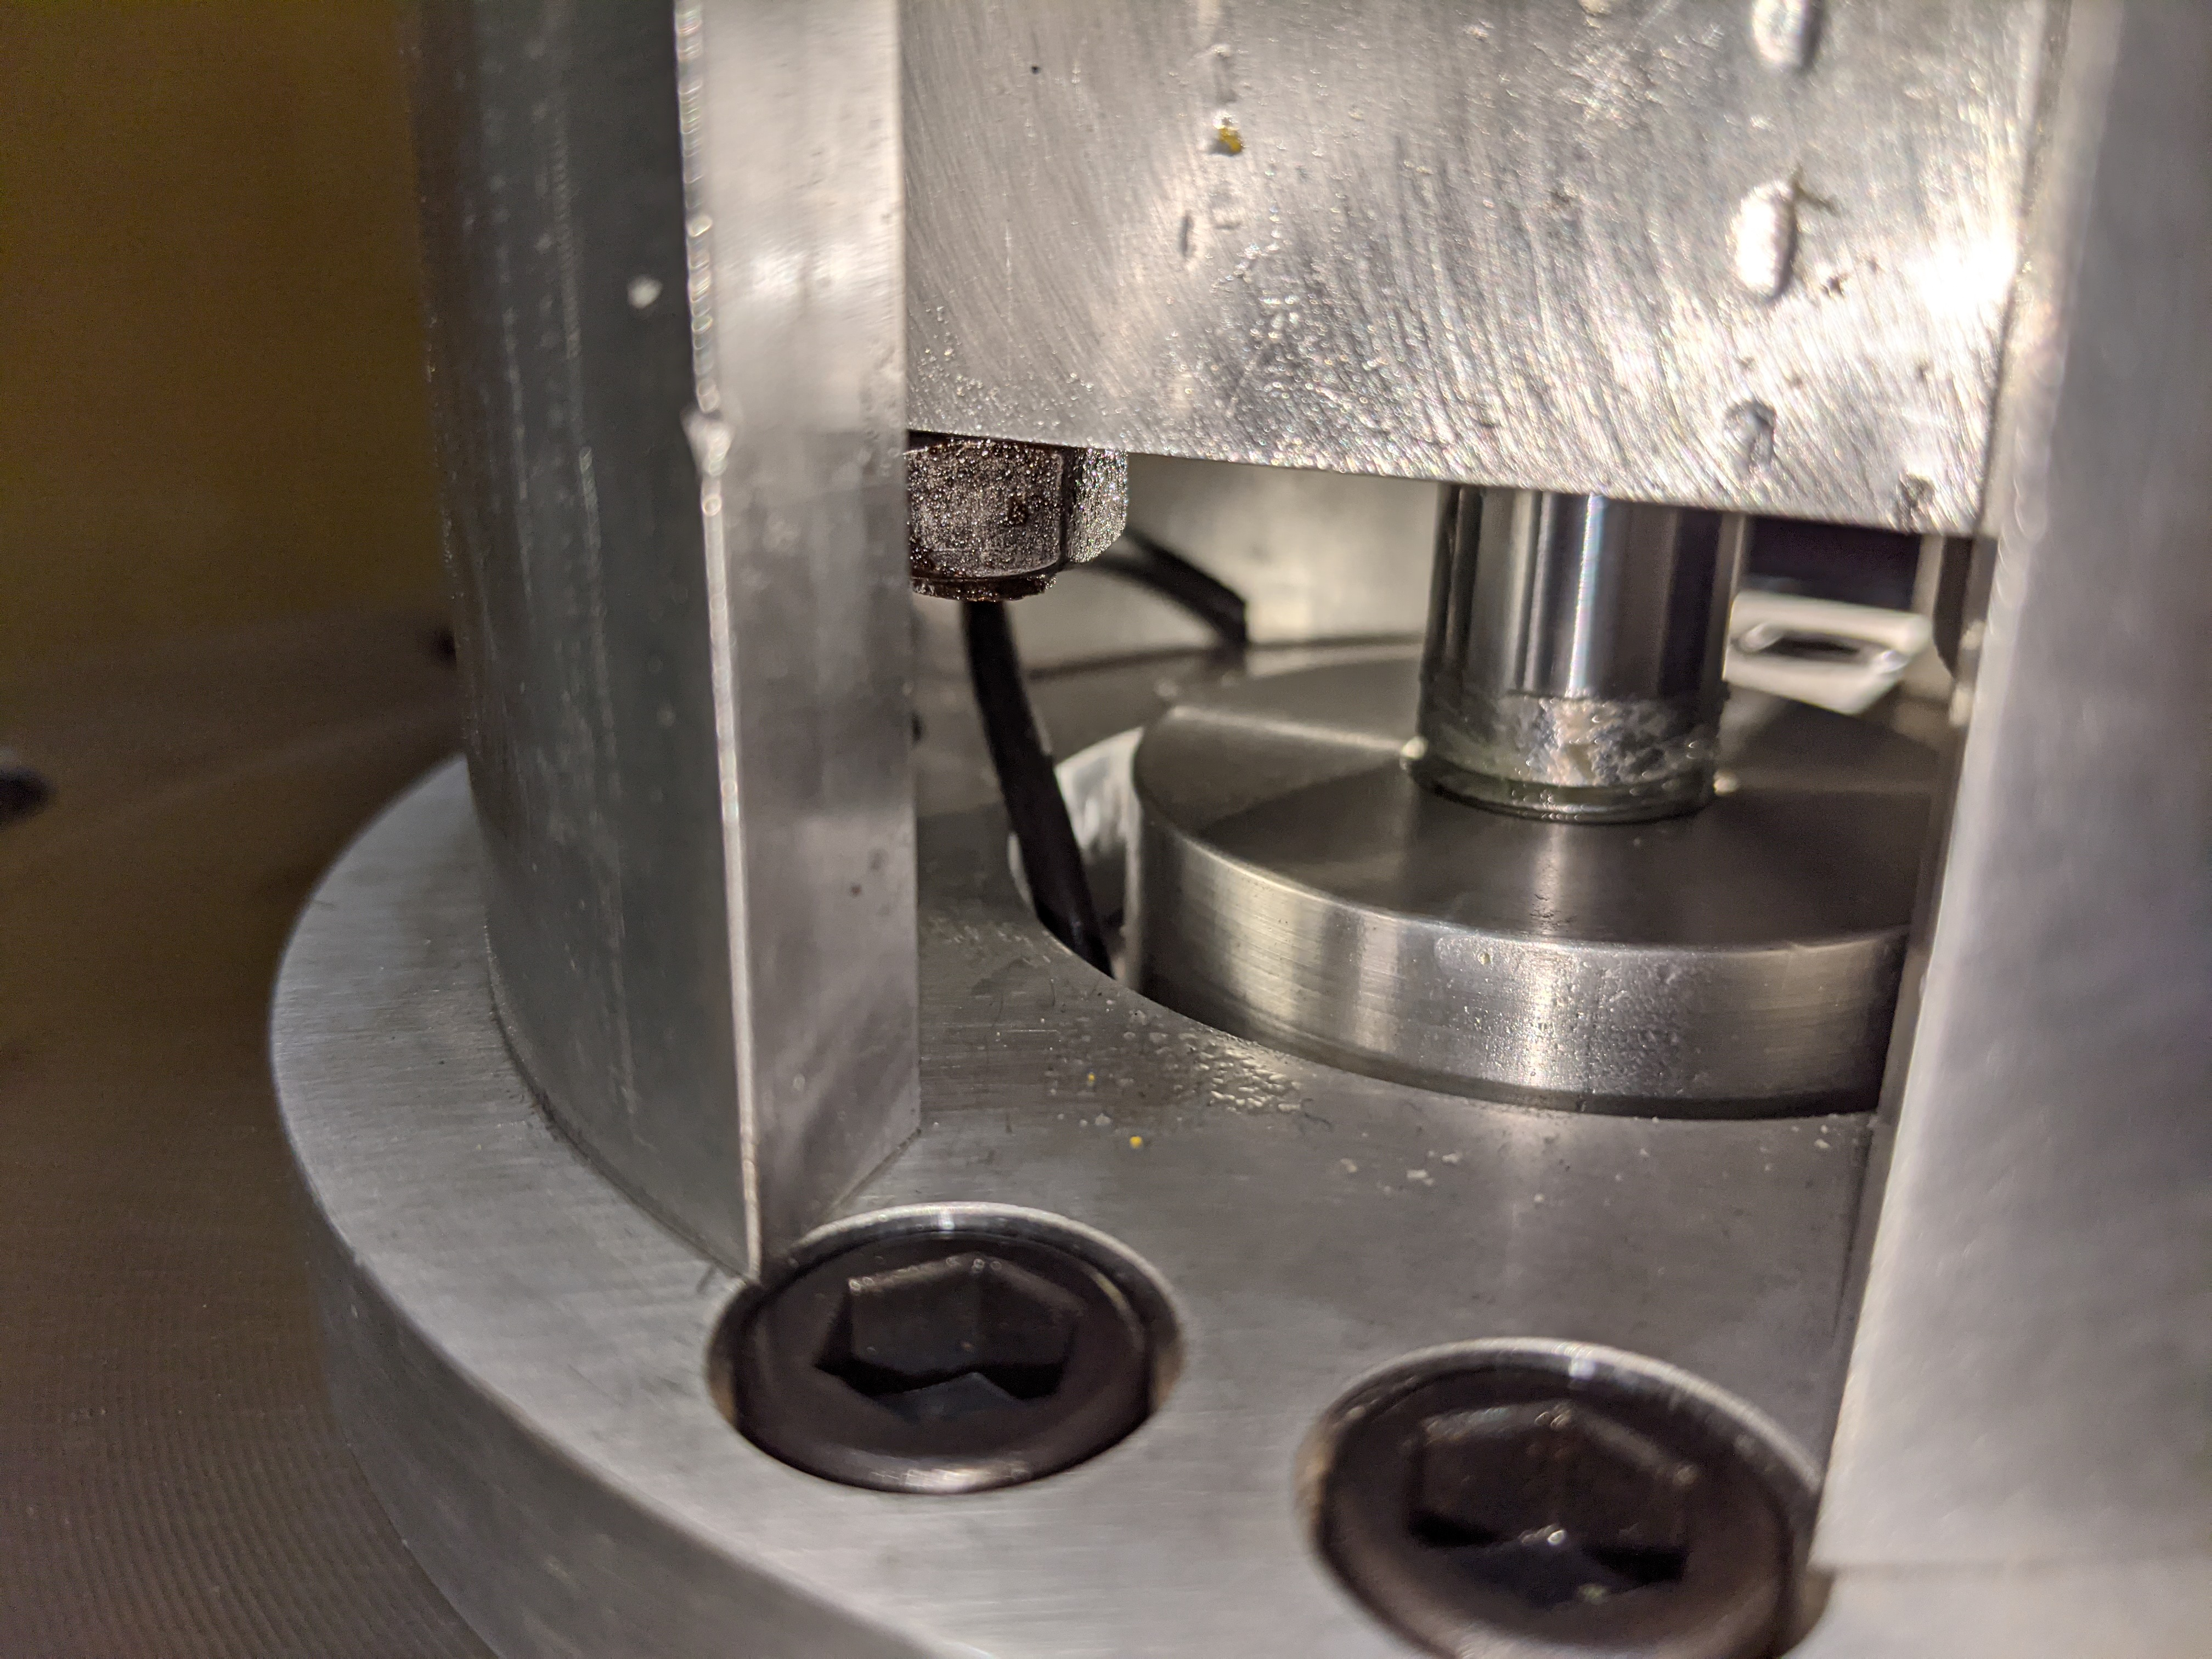
\includegraphics[width=4.032in, height=3.024in]{design/photos/Piston_Broken_Oring.jpg}
    \caption{Broken o-ring (FFKM) in piston assembly.}
    \label{fig:broken oring piston}
    \vspace{16pt}
\end{figure}

    

\begin{figure}[htpb]
    \vspace{16pt}
    \centering
    \begin{subfigure}[t]{0.45\textwidth}
        \centering
        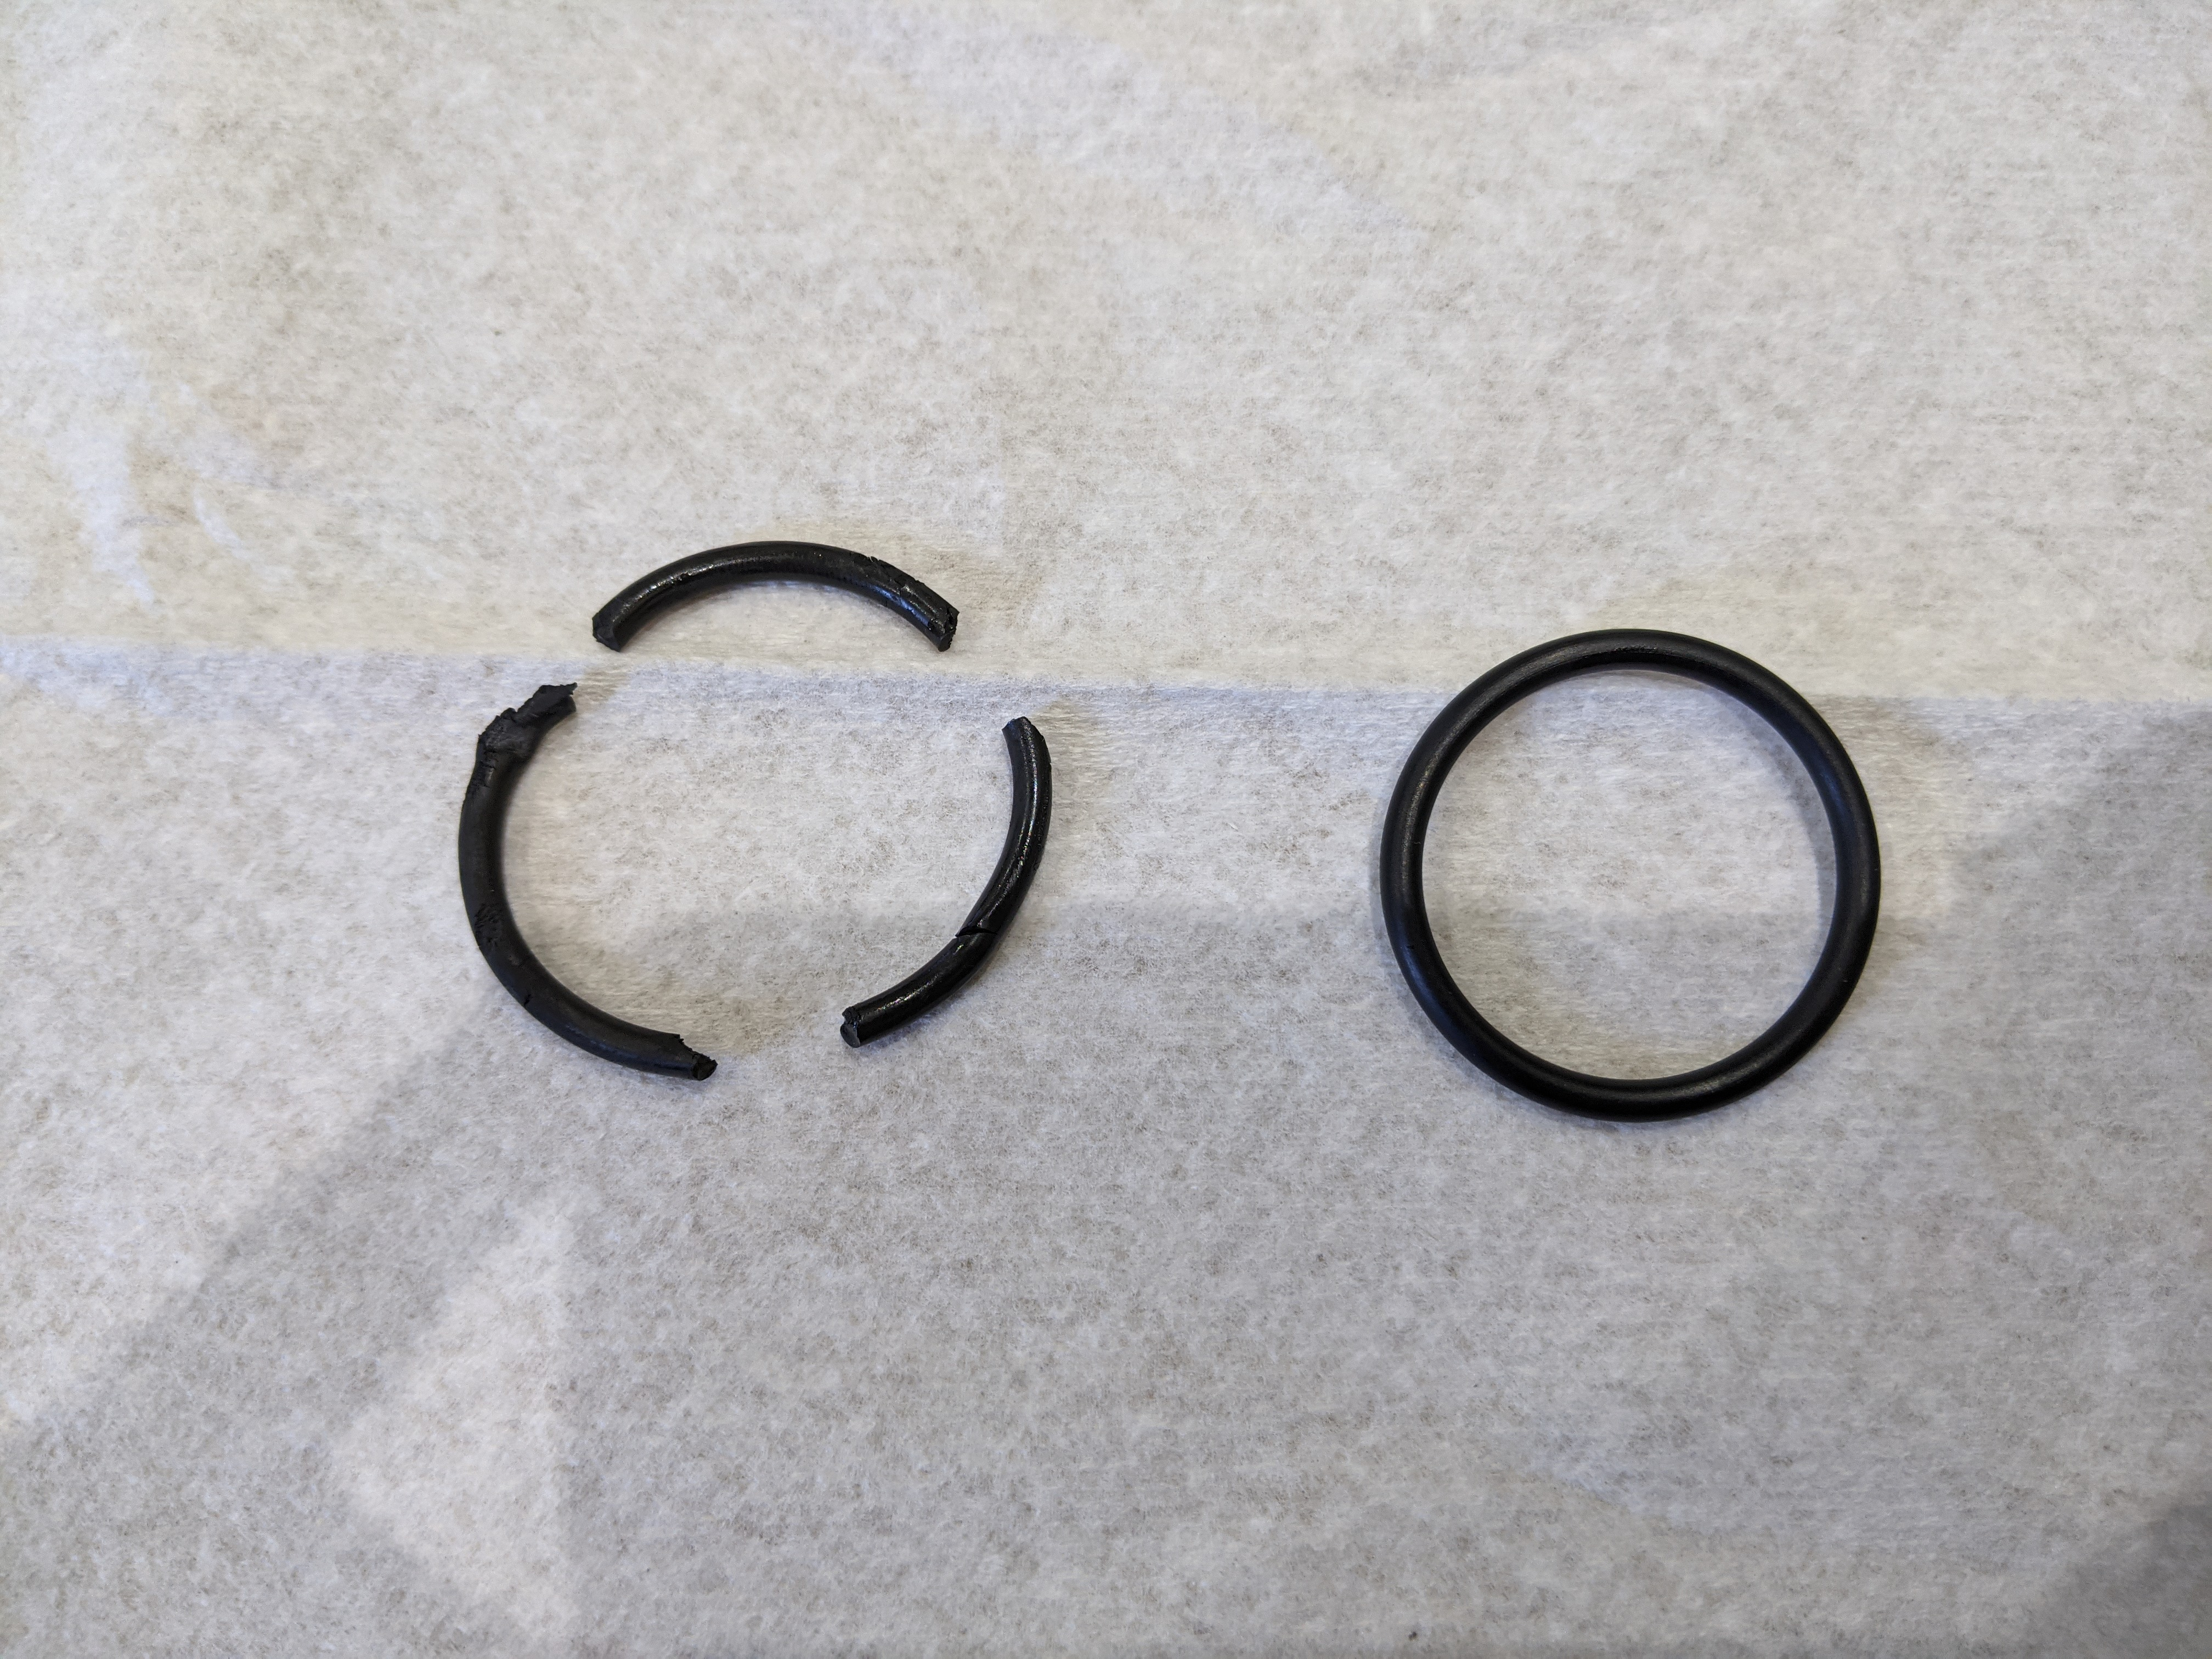
\includegraphics[width=\textwidth]{design/photos/Broken_Oring_Comparison.jpg}
        \caption{Comparison of broken o-ring (Nitrile) and new o-ring (FFKM).}
        \label{fig:broken oring comp}
    \end{subfigure}
    \hfill
    \begin{subfigure}[t]{0.45\textwidth}
        \centering
        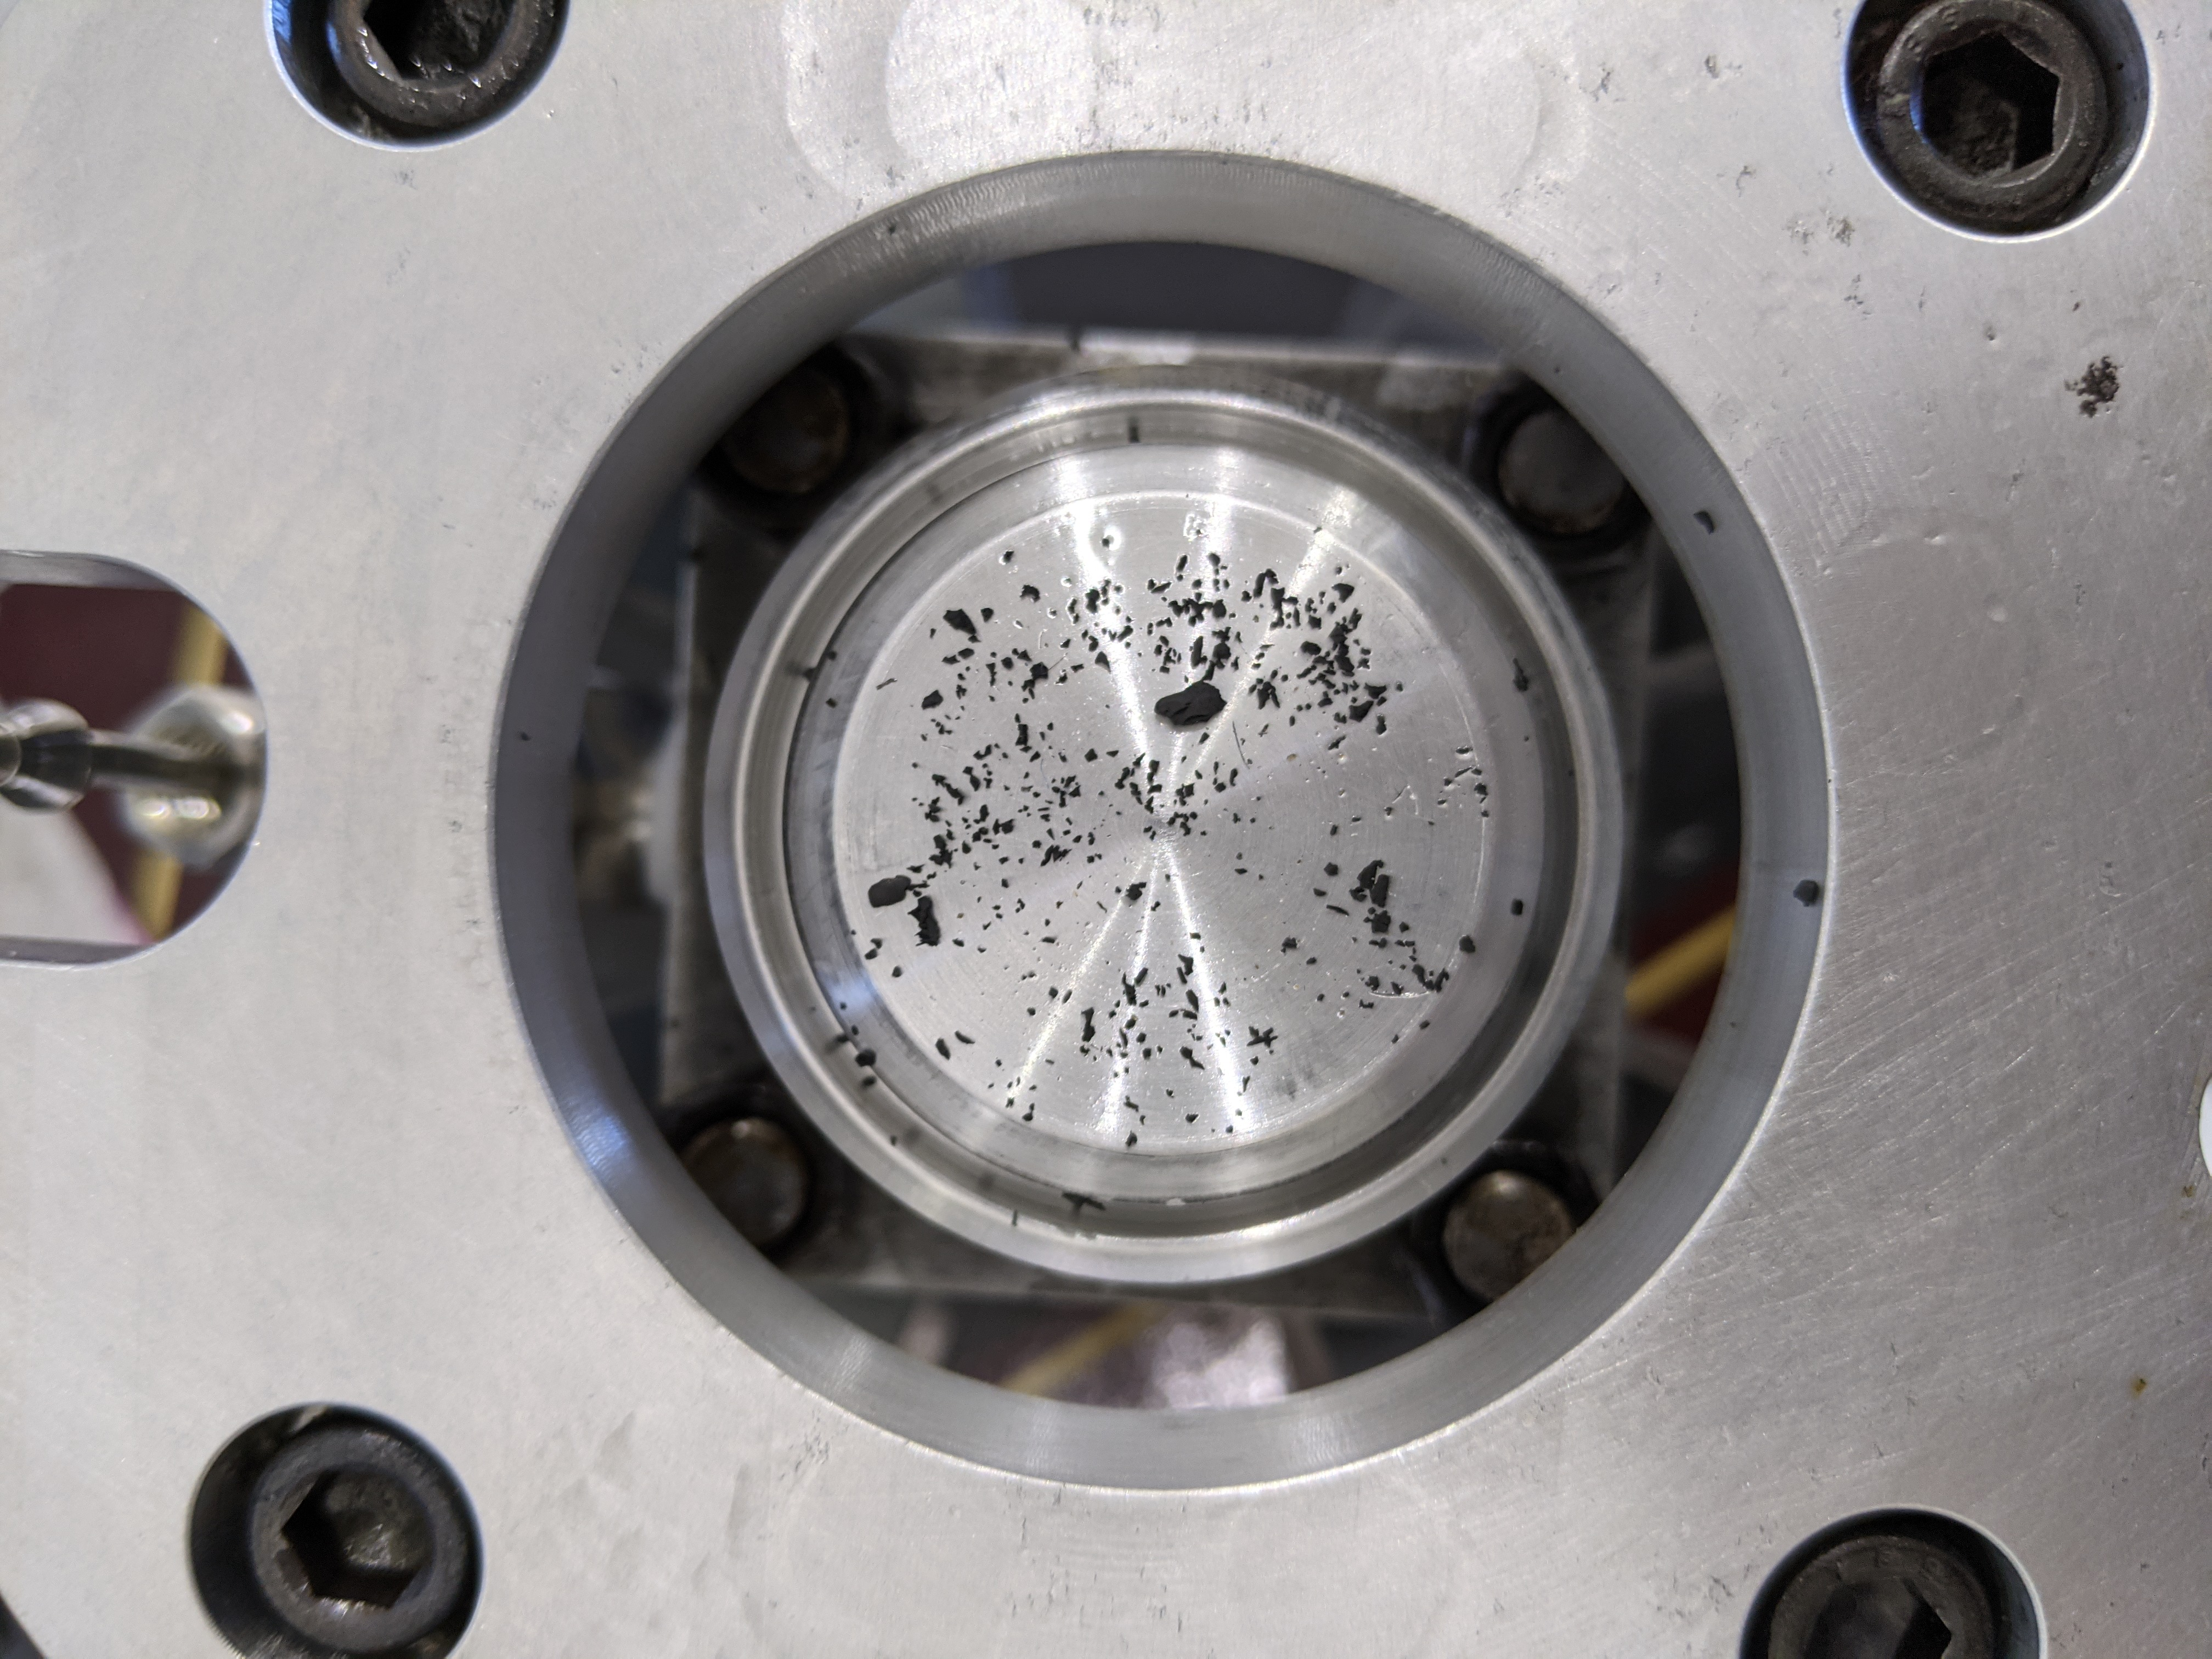
\includegraphics[width=\textwidth]{design/photos/Oring_Dust_Plug.jpg}
        \caption{Rubber dust from broken o-ring (Nitrile) on the top of the plug.}
        \label{fig:broken oring dust}
    \end{subfigure}
    \caption{Images of the aftermath of an o-ring failing during a 1000 psia test.}
    \label{fig:broken oring 2}
    \vspace{16pt}
\end{figure}
%



%%%%%%%%%%%%%%%%%%%%%%%%%%%%%%%%%%%%%%%%%%%%%%%%%%%%%%%%%%%%%%%%%%%%%%%
%%%%%%%%%%%%%%%%%%%%%%%%%%%% EXPERIMENT %%%%%%%%%%%%%%%%%%%%%%%%%%%%%%%
%%%%%%%%%%%%%%%%%%%%%%%%%%%%%%%%%%%%%%%%%%%%%%%%%%%%%%%%%%%%%%%%%%%%%%%
% discuss experimental set up, differences between this set up and the previous rupture disk set up
% discuss differences in piston valve iterations and why changes were made
% pictures and stuff
% maybe test matrix?
\section{Experimental Facility and Methodology} \label{s:experiment}

This section will describe the experimental facility, highlighting the modifications from the rupture disk experiments, and the methodology used to test the piston valve.

% talk about basic methodology of experiments and testing, introduce the structure of the section


% section for experimental facility, comparison of rupture disk and piston valve test set ups
\subsection{Experimental Facility} \label{ss:facility}

% P&ID, photos, etc. of facility -- highlight differences between burst disk and piston
The main facility, seen in \Cref{fig:HENRI Facility}, is set up similarly to a shock tube, with a driver tank on the floor, an intermediate tube section, a test section, and a reflector section. The whole facility is upside-down to the HENRI cartridge orientation in the TREAT core. In the reactor, the driver tank will be above the core with the test section in the fuel. The reflector section will extend past the fuel to provide space for the gas reflection effects outside of the active region in the core. The intermediate section allows for the driver tank to be positioned above the reactor core while also decreasing the total required volume of helium-3 for the HENRI system. The facility is made using 304 stainless steel. The test section and reflector are pipe with a \SI{4.826}{\centi\meter} outer diameter and \SI{0.368}{\centi\meter} wall thickness (1.5 inch schedule 40 NPS); the intermediate section is \SI{3.175}{\centi\meter} (1.25 inch) outer diameter tubing with \SI{0.3175}{\centi\meter} ($0.125$ inch) wall thickness; and the driver tank is pipe with a \SI{16.8275}{\centi\meter} outer diameter and \SI{0.7112}{\centi\meter} wall thickness (6 inch schedule 40 NPS). The piston valve is attached to the top flange of the driver tank and hangs inside.\Cref{fig:piston valve} shows the piston valve attached to the driver tank flange, outside of the HENRI cartridge. This setup is used to test the operation of the valve, as well as the durability and re-usability of the valve. Performing these tests outside of the cartridge allows for easier observation and decreases time between durability tests.

%
\begin{figure}[htbp]
    \vspace{16pt}
    \centering
    \begin{subfigure}[t]{0.6\textwidth}
        \centering
        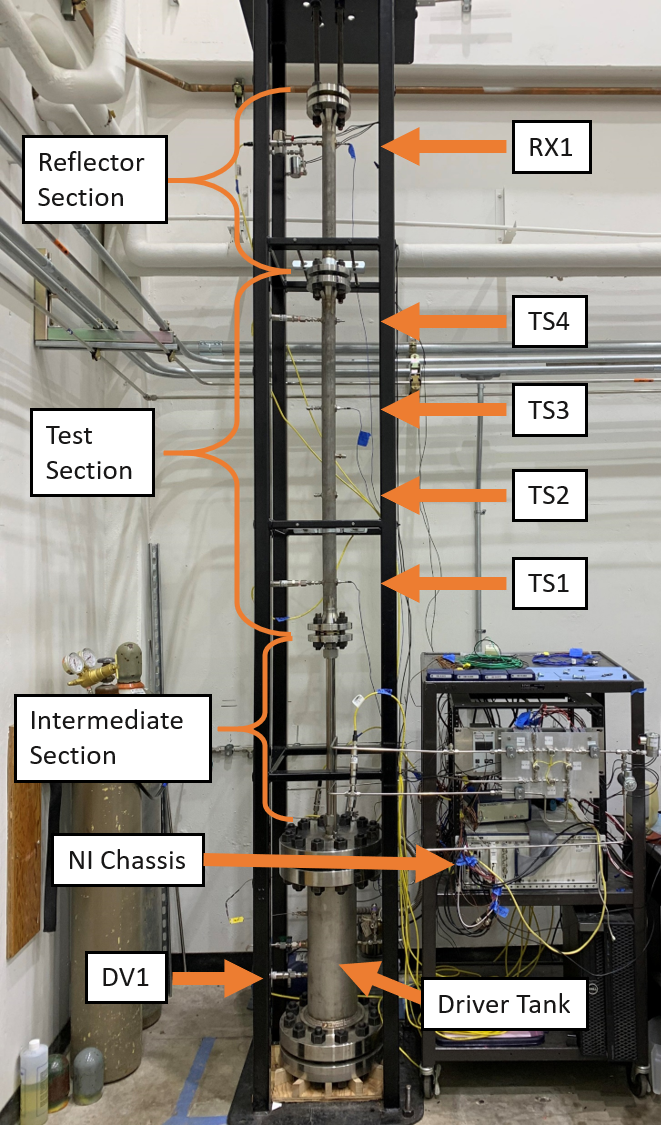
\includegraphics[width=2in]{experiment/photos/HENRI_labels.png}
        \caption{HENRI out-of-pile experimental facility.}
        \label{fig:HENRI Facility}
    \end{subfigure}
    \hfill
    \begin{subfigure}[t]{0.35\textwidth}
        \centering
        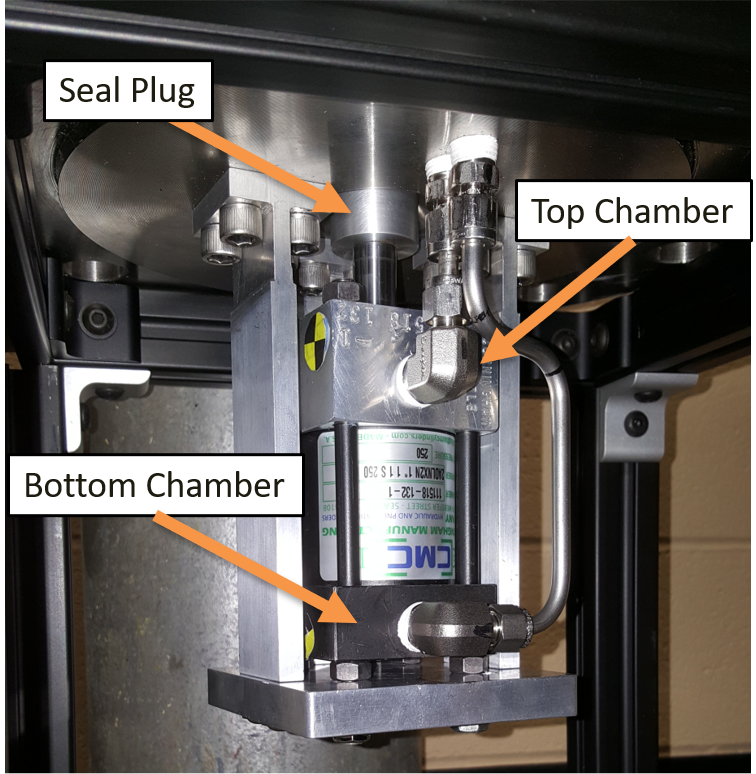
\includegraphics[width=0.9\textwidth]{design/photos/piston_mount_chambers.png}
        \caption{Piston valve attached to driver tank flange with mount, used for seal durability testing.}
        \label{fig:piston valve}
    \end{subfigure}
    \caption{HENRI experimental facility for piston valve testing.}
    \label{fig:facility}
    \vspace{16pt}
\end{figure}
%



The facility has pressure transducers distributed along its length, the major positions are highlighted in \Cref{fig:HENRI Facility}, and 1 thermocouple in the driver tank. The pressure transducers are one of two main types: Omega PX459 or PCB 113B24. All of the Omega pressure transducers are 0-\SI{10.3}{\mega\pascal} (0-1500 psia), except for two: a 0-\SI{24.1}{\mega\pascal} (0-3500 psia) transducer used on the driver tank, and a 0-\SI{0.103}{\mega\pascal} (0-15 psia) transducer used for the vacuum line. The Omega pressure transducers output a current from 4-\SI{20}{\milli\amp}, which is converted to voltage using a \SI{250}{\ohm} shunt resistor. The PCB transducers output a signal that is sent through a PCB Model 482C signal conditioner before being output to the voltage card. The data acquisition system uses a National Instruments (NI) PXIe-1085 chassis with a NI PXIe-8135 controller, a NI PXIe-4303 voltage input card for reading the instrumentation, and a NI PXI-6515 digital output card for controlling the solenoid valves. A LabVIEW program is used to record data from the chassis and to control the solenoid valves. A piping and instrumentation diagram (P\&ID) for operating the piston valve can be seen in \Cref{fig:sv pid}. There is a manifold of four (4) solenoid valves used to operate the piston. SV-PI2 and SV-PI4 open to fill the top and bottom chamber, respectively; and SV-PI1 and SV-PI3 open to vent the top and bottom chamber, respectively. These solenoid valves are Parker Series 9 Miniature Calibrant Valve 009-0172-900. This particular valve was selected for its small form factor, high pressure rating of \SI{8.6}{\mega\pascal}(1250 psi), and low helium leak rate of \SI{1e-7}{atm\ \centi\meter^3\per\second}.

% %
% \begin{figure}[htbp]
%     \vspace{16pt}
%     \centering
%     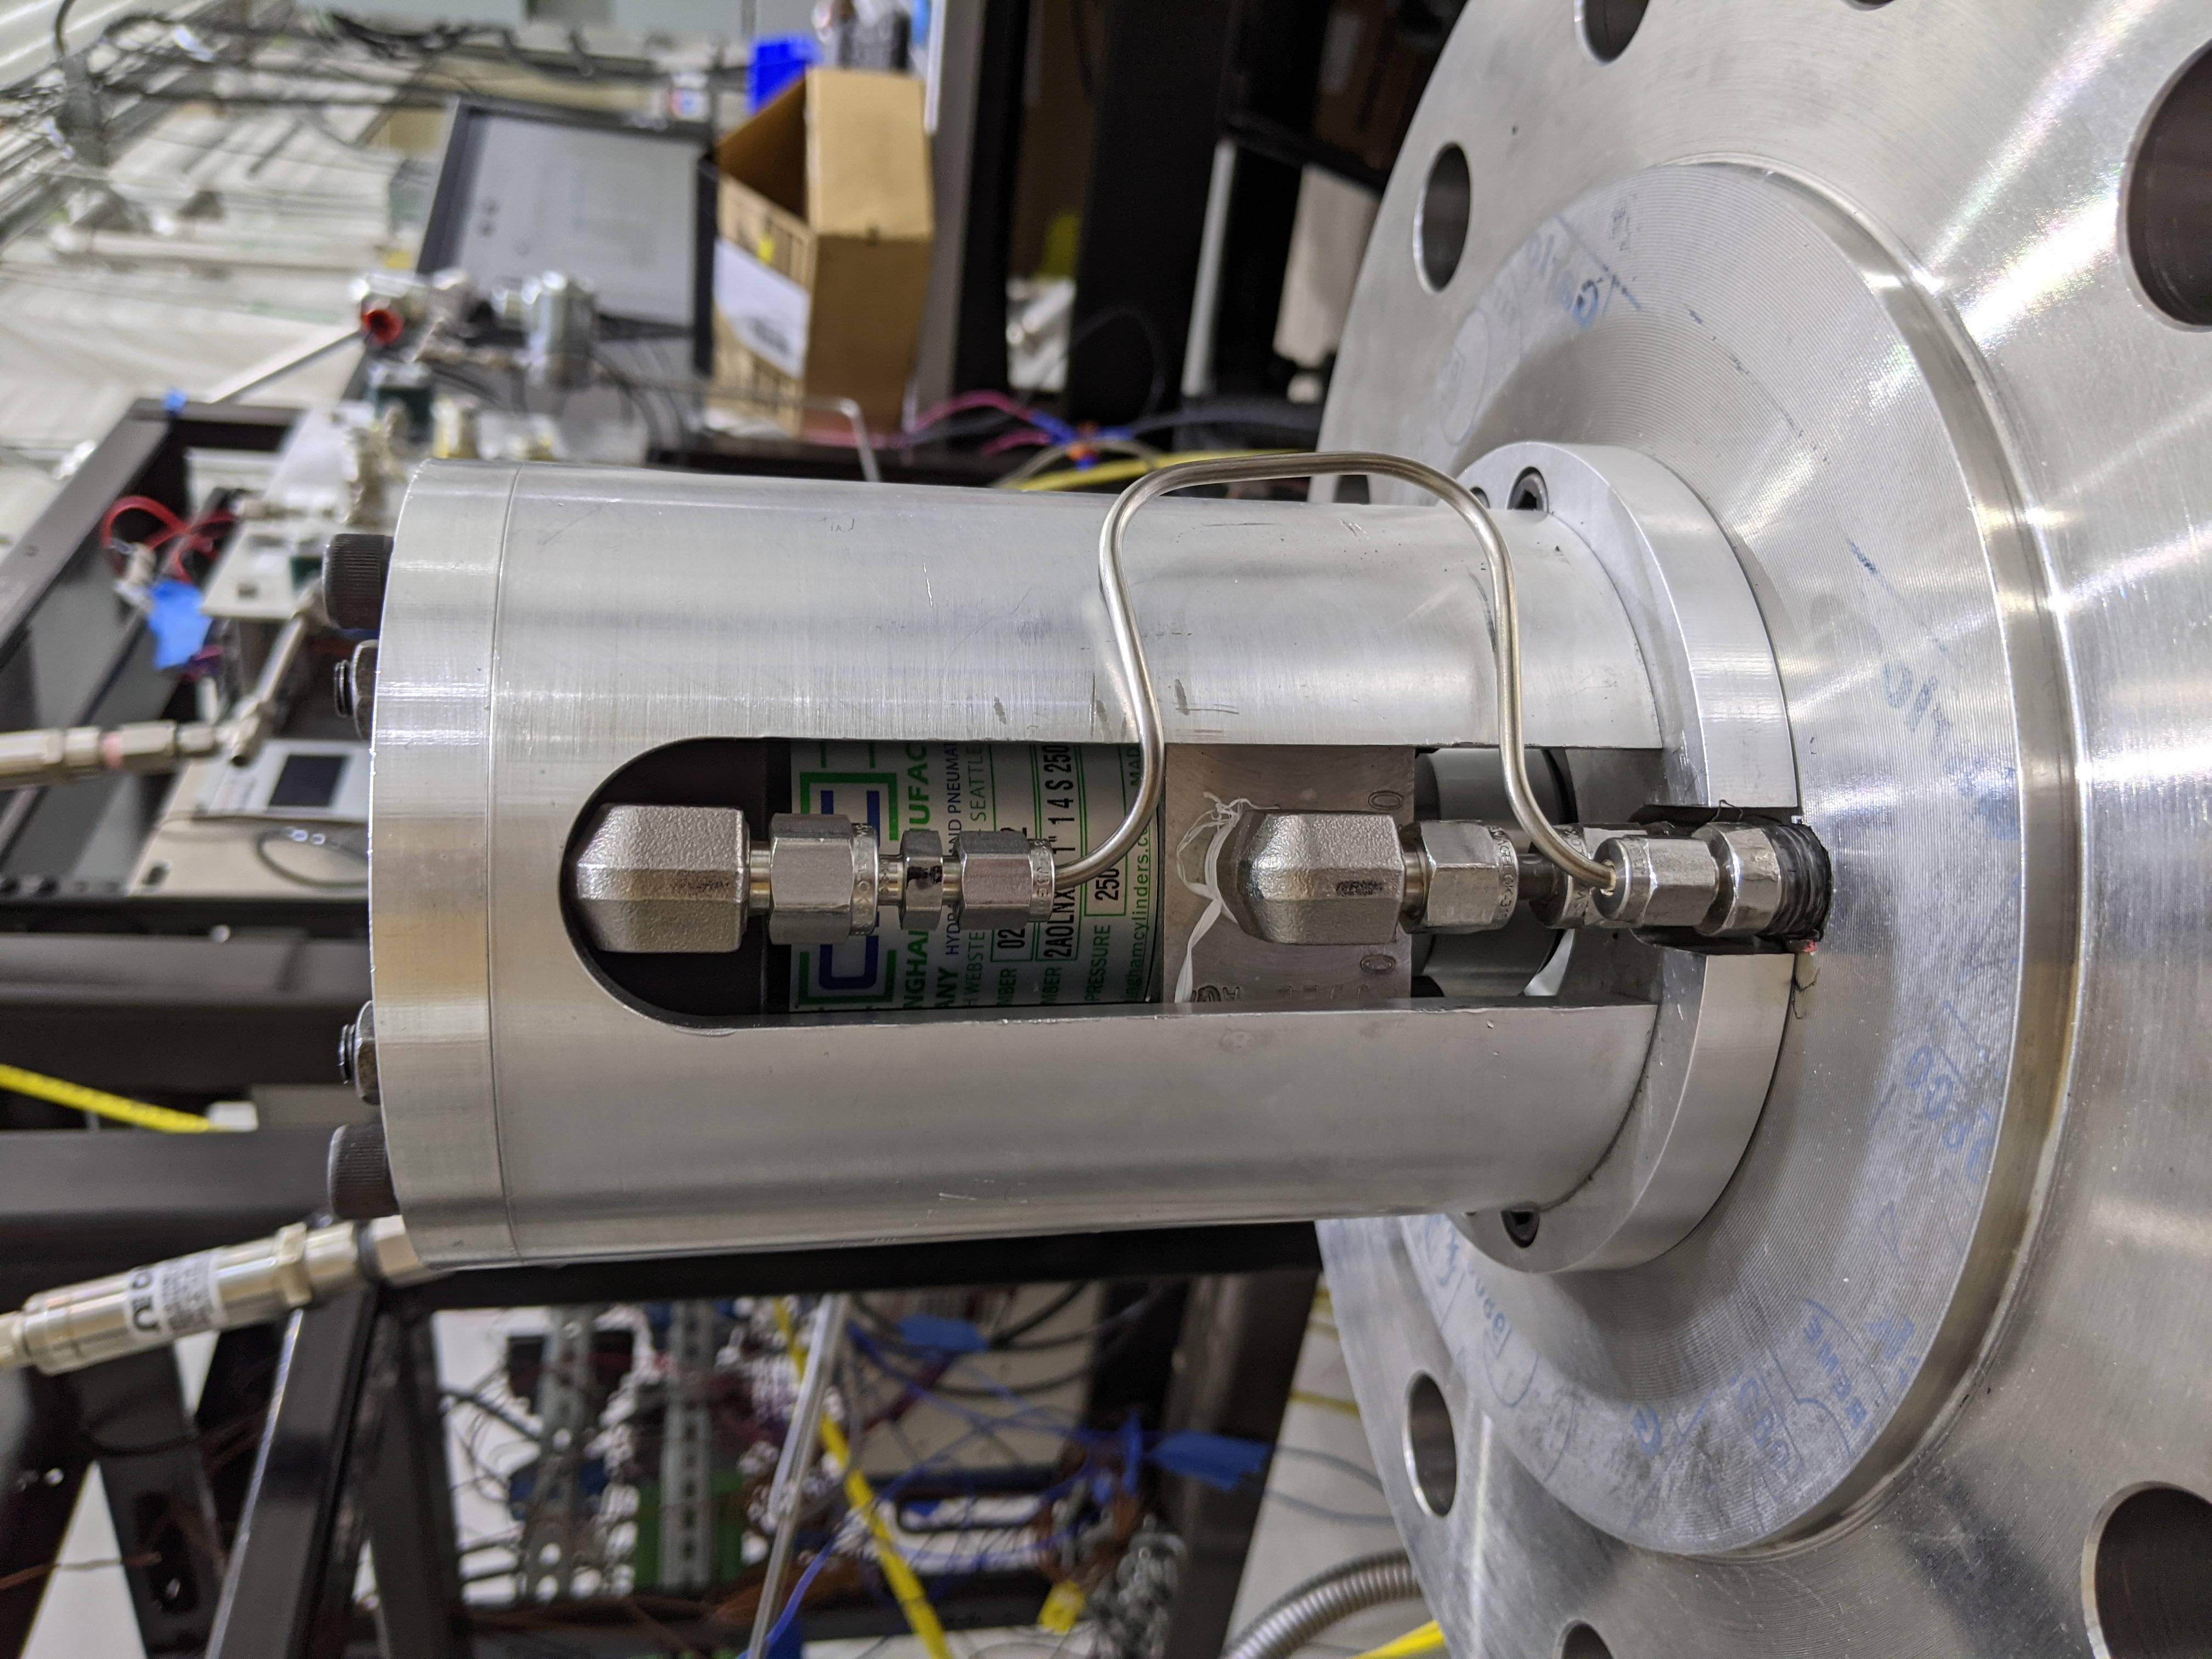
\includegraphics[width=3.024in, height=4.032in]{experiment/photos/Piston_Assembly.jpg}
%     \caption{Piston assembled with second generation mount on flange.}
%     \label{fig:piston assembly}
%     \vspace{16pt}
% \end{figure}
% %


%
\begin{figure}[htbp]
    \vspace{16pt}
    \centering
    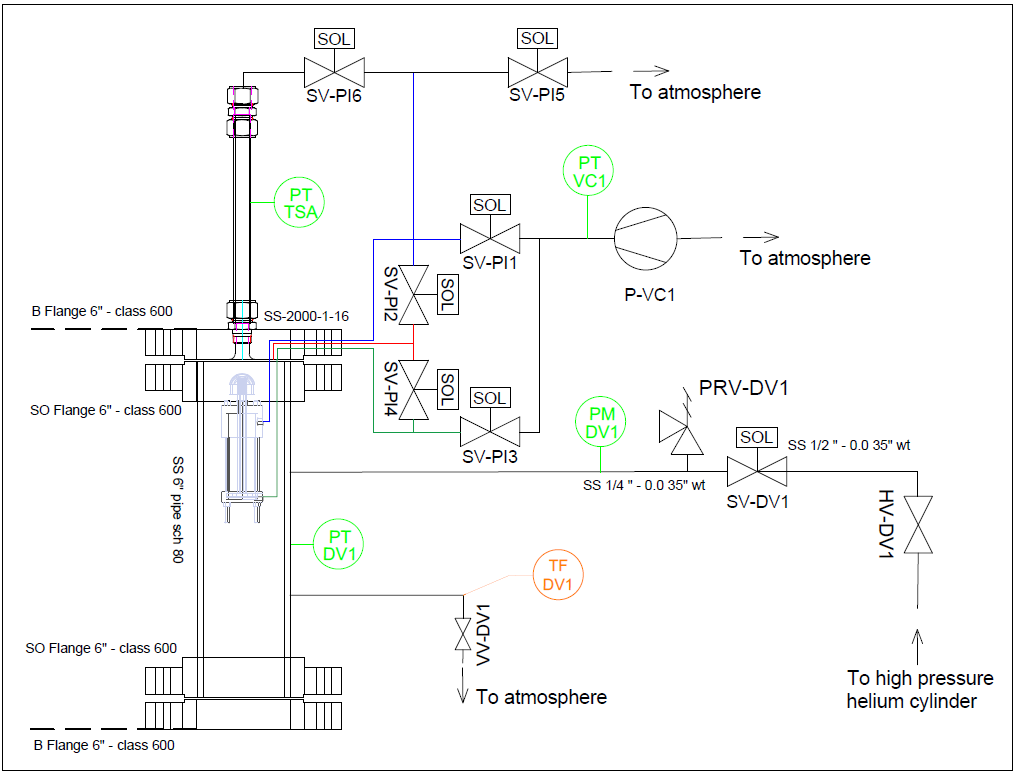
\includegraphics[width=0.6\textwidth]{experiment/photos/HENRI_valve_PID.PNG}
    \caption{Piping and instrumentation diagram (P\&ID) for piston valve operation.}
    \label{fig:sv pid}
    \vspace{16pt}
\end{figure}
%




% section for detailed experimental method (test matrix)
\subsection{Experimental Methodology} \label{ss:methodology}

% we tested the plugs and o-rings for durability / sealing with sustained seal tests and repeated seal tests outside of the henri facility (just using the flange and piston)
% we tested the valve / plugs / o-rings in henri tests

The overall methodology for testing the piston valve includes two main parts: testing the piston valve's repeatability in HENRI helium insertions; and testing the piston valve for re-usability and sealing after large numbers of cycles. The piston valve is first tested in a HENRI injection and the results are compared to those of the rupture disk tests to ensure the piston valve is performing correctly and pressurizing the cartridge to the desired \SI{1.72}{\mega\pascal} (250 psi) in \SI{5}{\milli\second}. Secondly, the piston valve is tested repeatedly at one initial pressure to determine the repeatability of the valve, then it is tested at different initial pressures to determine how predictable the piston valve's behaviour is over a range of operating pressure. Testing the re-usability of the piston valve was performed by cycling the piston valve to simulate the wear of long term use and comparing its sealing ability before and after the cycles. The LabVIEW code used for data acquisition was modified to automate the piston cycling process, so the cycle test could be performed overnight, then the piston valve is tested the next day to determine the seal degradation due to wear.



%%%%%%%%%%%%%%%%%%%%%%%%%%%%%%%%%%%%%%%%%%%%%%%%%%%%%%%%%%%%%%%%%%%%%%%
%%%%%%%%%%%%%%%%%%%%%%%%%%%%% RESULTS %%%%%%%%%%%%%%%%%%%%%%%%%%%%%%%%%
%%%%%%%%%%%%%%%%%%%%%%%%%%%%%%%%%%%%%%%%%%%%%%%%%%%%%%%%%%%%%%%%%%%%%%%
% discuss / compare results to previous rupture disk stuff and previous iteration of piston valve
\section{Results and Discussion} \label{s:results}
This section will present the results of the work and discuss their significance. The piston valve is first compared to the previous results using the rupture disks to ensure the valve works as intended and provides the desired pressurization. Then, the piston valve is compared to itself to determine the valve's repeatability and predictability. The valve is then tested for re-usability and durability.

% subsection about piston v rupture disk
\subsection{Piston Valve Compared to Rupture Disk} \label{s:disk v piston}
The rupture disks were used in the HENRI system to determine if the system was capable of pressurizing to \SI{1724}{\kilo\pascal} (\SI{250}{psi}) in the desired time frame of \SI{5}{\milli\second}\cite{HeNURETH}. One of the goals of the piston valve is to open quickly enough to maintain as close to rupture disk physics as possible. 
%Computational fluid dynamics (CFD) simulations were validated using these experiments \cite{CFDNureth,HENRIATH}[MIGHT NEED DIFF REF HERE].
\Cref{fig:piston v disk} compares the results of a rupture disk test and a piston valve test, both with initial driver tank pressure of \SI{6.9}{\mega\pascal} (\SI{1000}{psia}) and intermediate tube inner diameter of \SI{2.54}{\centi\meter} (\SI{1}{inch}). The piston valve demonstrates that is able to reach the desired pressure of \SI{1.72}{\mega\pascal} (250 psi) in less than \SI{5}{\milli\second}. The piston valve opens quickly enough to replicate the pressure evolution observed in the rupture disks and performs well enough to move on with testing.

\begin{figure}[htbp]
    \vspace{16pt}
    \centering
    \begin{subfigure}[t]{0.45\textwidth}
        \centering
        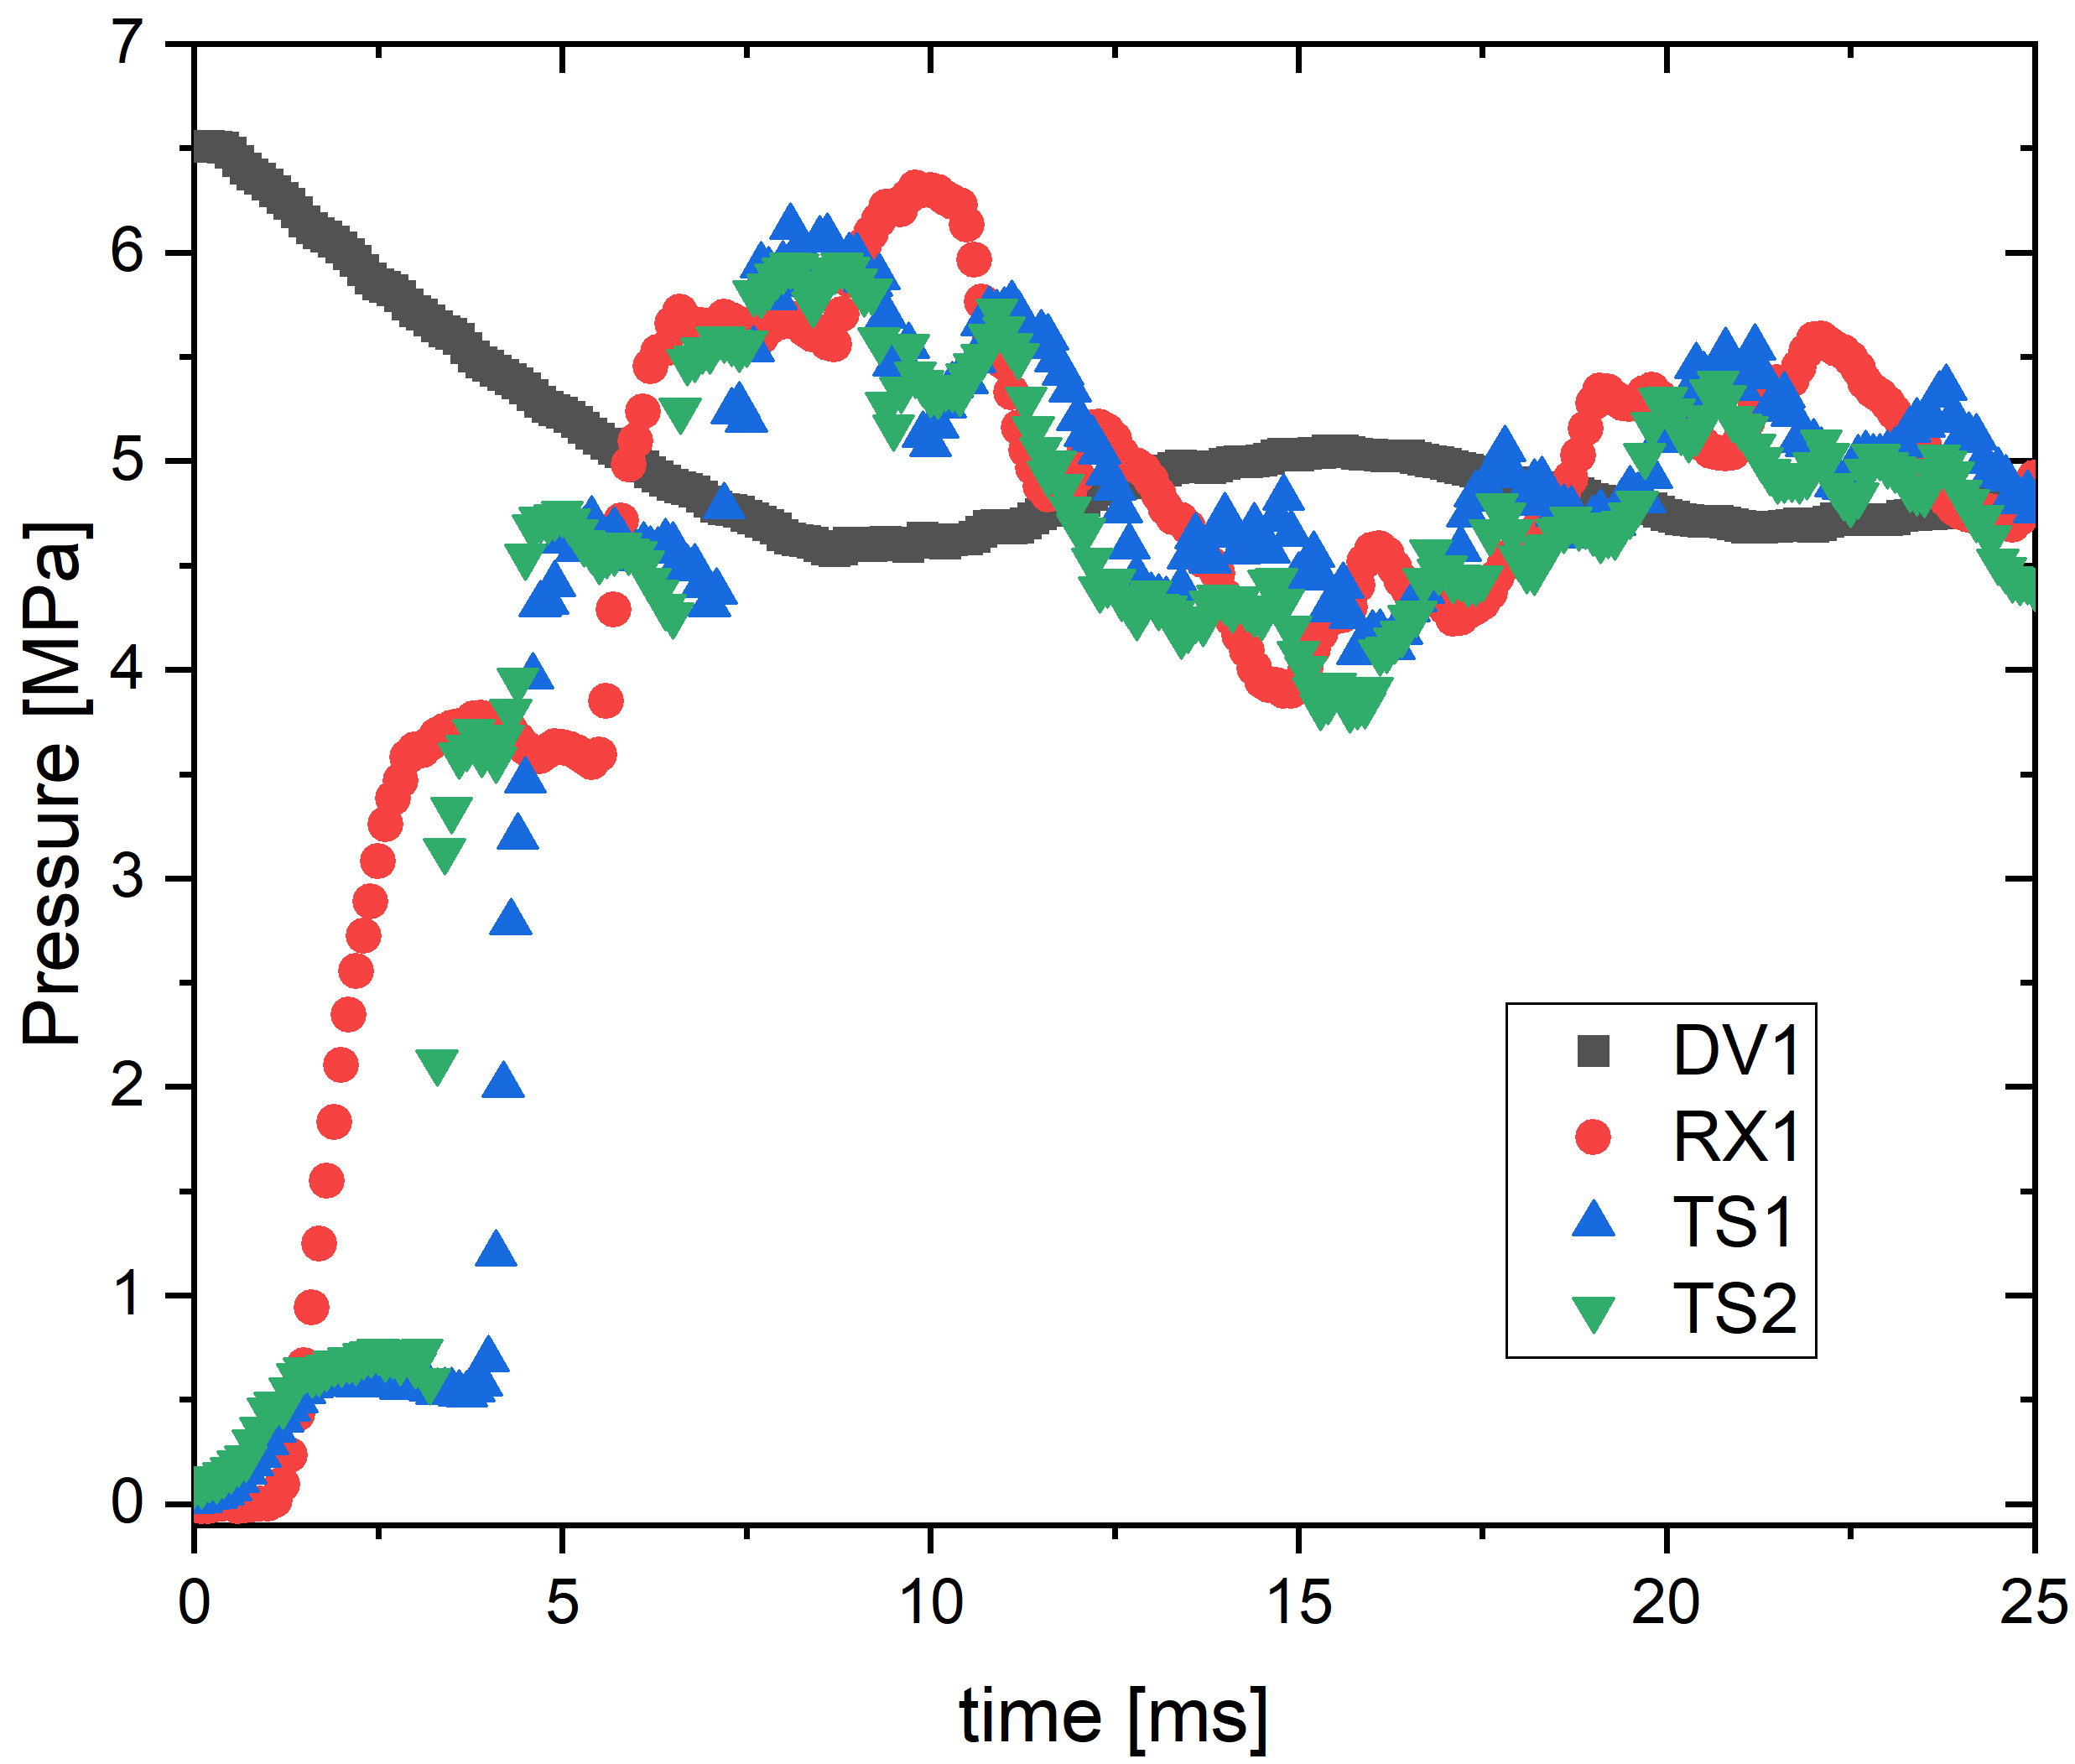
\includegraphics[width=0.9\textwidth]{results/plots/940psi-BD-1.png}
        \caption{Pressure over time for rupture disk HENRI test.}
        \label{fig:disk}
    \end{subfigure}
    \hfill
    \begin{subfigure}[t]{0.45\textwidth}
        \centering
        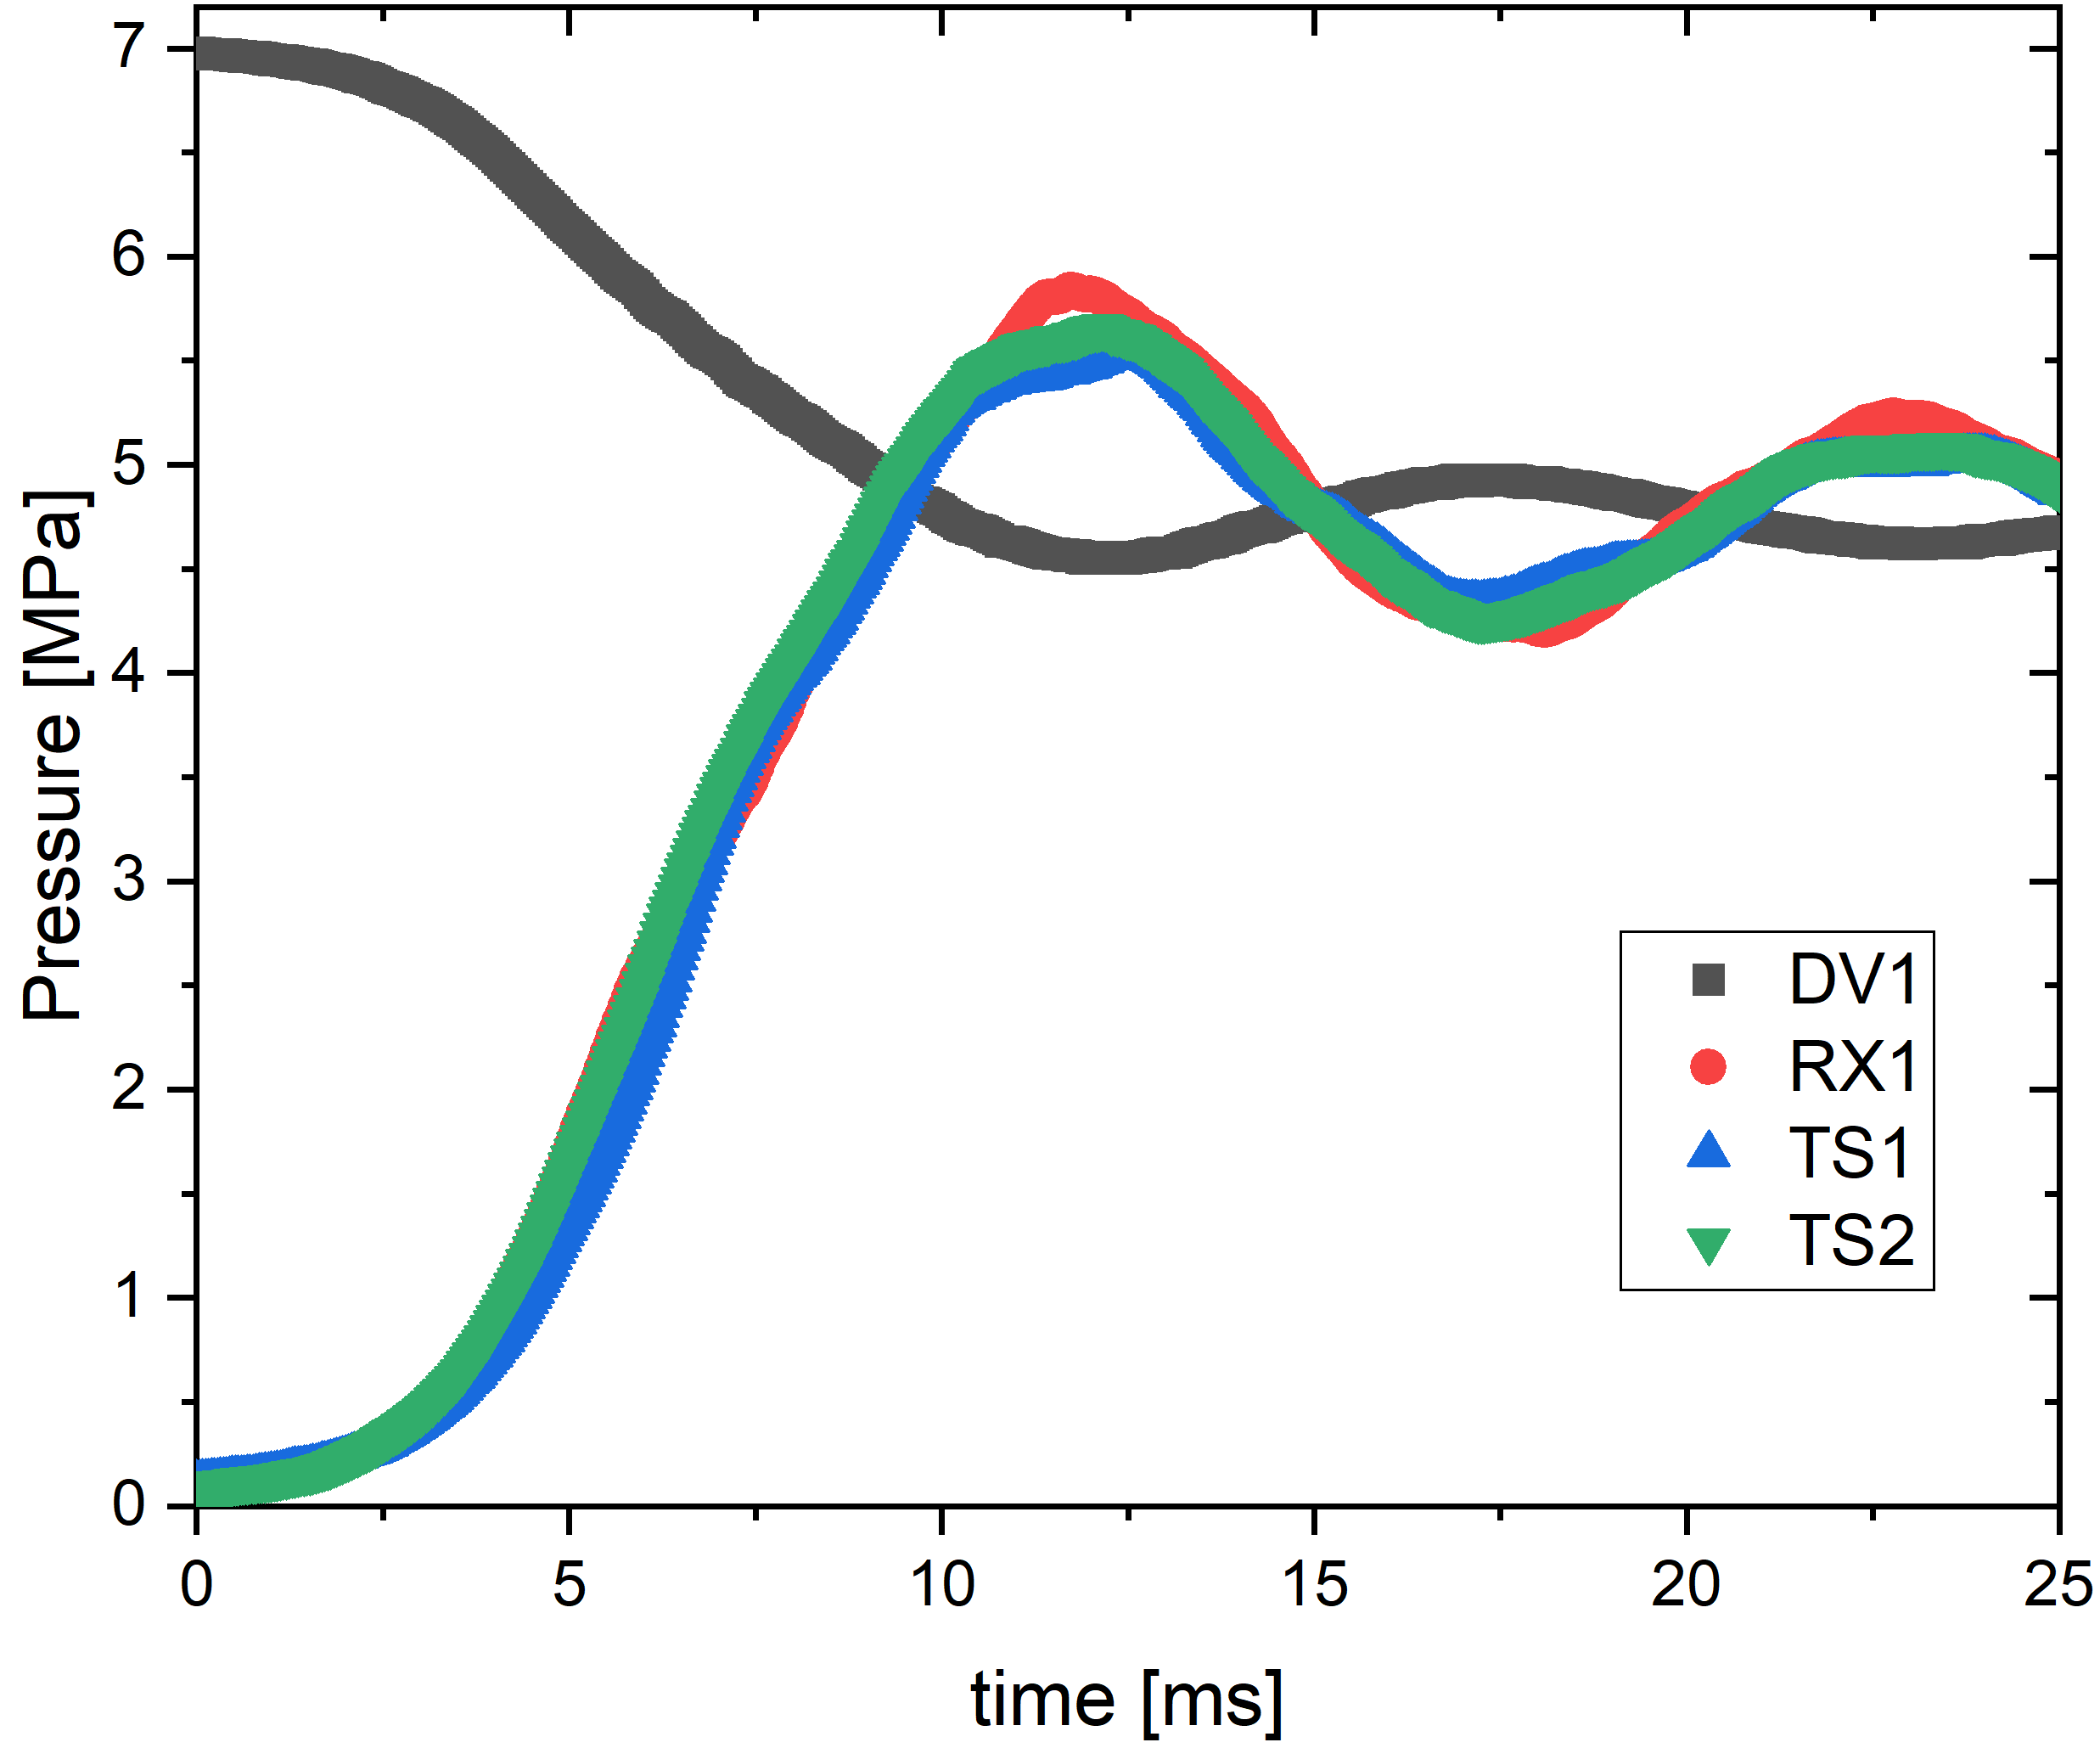
\includegraphics[width=0.9\textwidth]{results/plots/1000psi_mtM_Co.png}
        \caption{Pressure over time for a piston valve HENRI test.}
        \label{fig:piston metal 1000psi}
    \end{subfigure}
    
    \caption{Comparison of rupture disk and piston valve HENRI tests at an initial pressure of \SI{6.9}{\mega\pascal} (\SI{1000}{psia}) and with intermediate tube inner diameter of \SI{2.54}{\centi\meter} (\SI{1}{inch}).}
    \label{fig:piston v disk}
    \vspace{16pt}
\end{figure}



% first piston valve design
% the metal to metal seal did not last long -- durability issues, wear on the sealing surface, even with fancy materials; there was a small leak from the driver tank to the test section before the valve was fully open;
%%%%%%%%%%%%%%%%%%%%%%%%%%%%%%%%%%%%%%%%%%%%%%%%%%%%%%%%%%%%%%%%%%%%%%%%%%%%%%%%%%
% subsection about piston valve repeatability
\subsection{Piston Valve Repeatability} \label{ss:repeatability}
It is vital that the valve selected for the HENRI system will provide a repeatable and predictable pressurization of the cartridge during a TREAT transient. \Cref{fig:piston repeatability} shows results from two tests at the same initial pressure and multiple tests at different initial pressures, normalized by initial pressure. The first plot, \Cref{fig:piston 2 test}, demonstrates the piston valve will provide a repeatable pressurization for each test in TREAT. The second plot, \Cref{fig:norm}, provides data to predict the pressurization speed and profile for the HENRI cartridge over a range of initial pressures.


\begin{figure}[htbp]
    \centering
    \begin{subfigure}[t]{0.45\textwidth}
        \centering
        %\includegraphics[width=0.9\textwidth]{}
        \caption{Comparison of two piston valve tests at an initial pressure of \SI{6.9}{\mega\pascal} (1000 psi).}
        \label{fig:piston 2 test}
    \end{subfigure}
    \hfill
    \begin{subfigure}[t]{0.45\textwidth}
        \centering
        %\includegraphics[width=0.9\textwidth]{}
        \caption{Piston valve test results, at position TS3, normalized by initial driver tank pressure for a range of initial driver tank pressures.}
        \label{fig:norm}
    \end{subfigure}
    \caption{Comparison of results for piston valve to demonstrate repeatability at one initial pressure and predictability at varying initial pressures.}
    \label{fig:piston repeatability}
\end{figure}

%%%%%%%%%%%%%%%%%%%%%%%%%%%%%%%%%%%%%%%%%%%%%%%%%%%%%%%%%%%%%%%%%%%%%%%%%%%%%%%%%%
% subsection about seal durability testing on the piston valve
\subsection{Piston Valve Re-usability} \label{ss:reusability}
The re-usability of the piston valve was tested by cycling the piston 500 times, then comparing the sealing capability to before the cycles. After 500 cycles, the piston valve would not hold a seal, even with over \SI{6.9}{\mega\pascal} (1000 psi) in the bottom chamber of the piston and in the driver tank. The valve needs to be able to be re-used without being replaced or maintained often, which is one of the reasons the rupture disks do not work. The metal plug was observed to have significant wear after the cycling tests, seen in \Cref{fig:plug wear}, which was asymmetrical. The used stainless steel plug, bottom left, has extreme asymmetrical wear, which meant that the plug could not be used to seal at any pressure. The wear on the aluminum plug was also asymmetrical, however the softer metal was worn more easily and the plug has a more defined ring around its circumference. The asymmetrical wear was attributed to the three legged piston mount that allowed the piston to move slightly in one direction when the valve closed. A new mount and a new plug design that does not wear as much, or can still seal after being worn, would solve this problem.

\begin{figure}[htbp]
    \vspace{16pt}
    \centering
    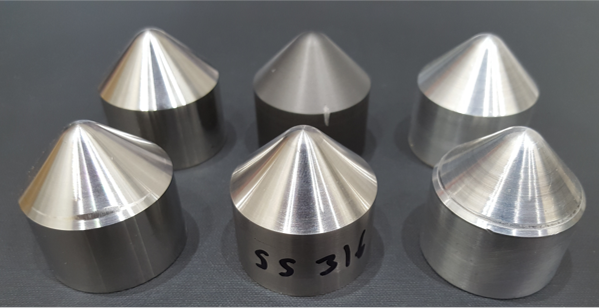
\includegraphics[width=0.6\textwidth]{design/photos/plug_gen1_wear.png}
    \caption{Assorted plugs for piston valve. Clockwise, starting at the top left: stainless steel, unused; anodized aluminum, unused; aluminum, unused; aluminum, used; stainless steel, lightly used; and stainless steel used.}
    \label{fig:plug wear}
    \vspace{16pt}
\end{figure}

%%%%%%%%%%%%%%%%%%%%%%%%%%%%%%%%%%%%%%%%%%%%%%%%%%%%%%%%%%%%%%%%%%%%%%%%%%%%%%%%%%
% subsection about new piston valve design
\subsection{Piston Valve Design Improvements} \label{ss:new valve}
The piston mount was redesigned to be as symmetrical as possible. The three legs were replaced by a single piece cylinder sandwiched by two plates. One plate attaches the cylinder to the piston and the other plate attaches the cylinder to the flange. The new mount can be seen in \Cref{fig:cad mount 2}. The new plug design has a dovetail groove to hold an o-ring, which will provide a better seal than the metal only plug, especially at low pressures. The o-ring will also maintain sealing capability after more cycles than just metal. \Cref{fig:plug v2 draw} shows a drawing of the new plug design.

\begin{figure}[htbp]
    \centering
    \begin{subfigure}[t]{0.45\textwidth}
        \centering
        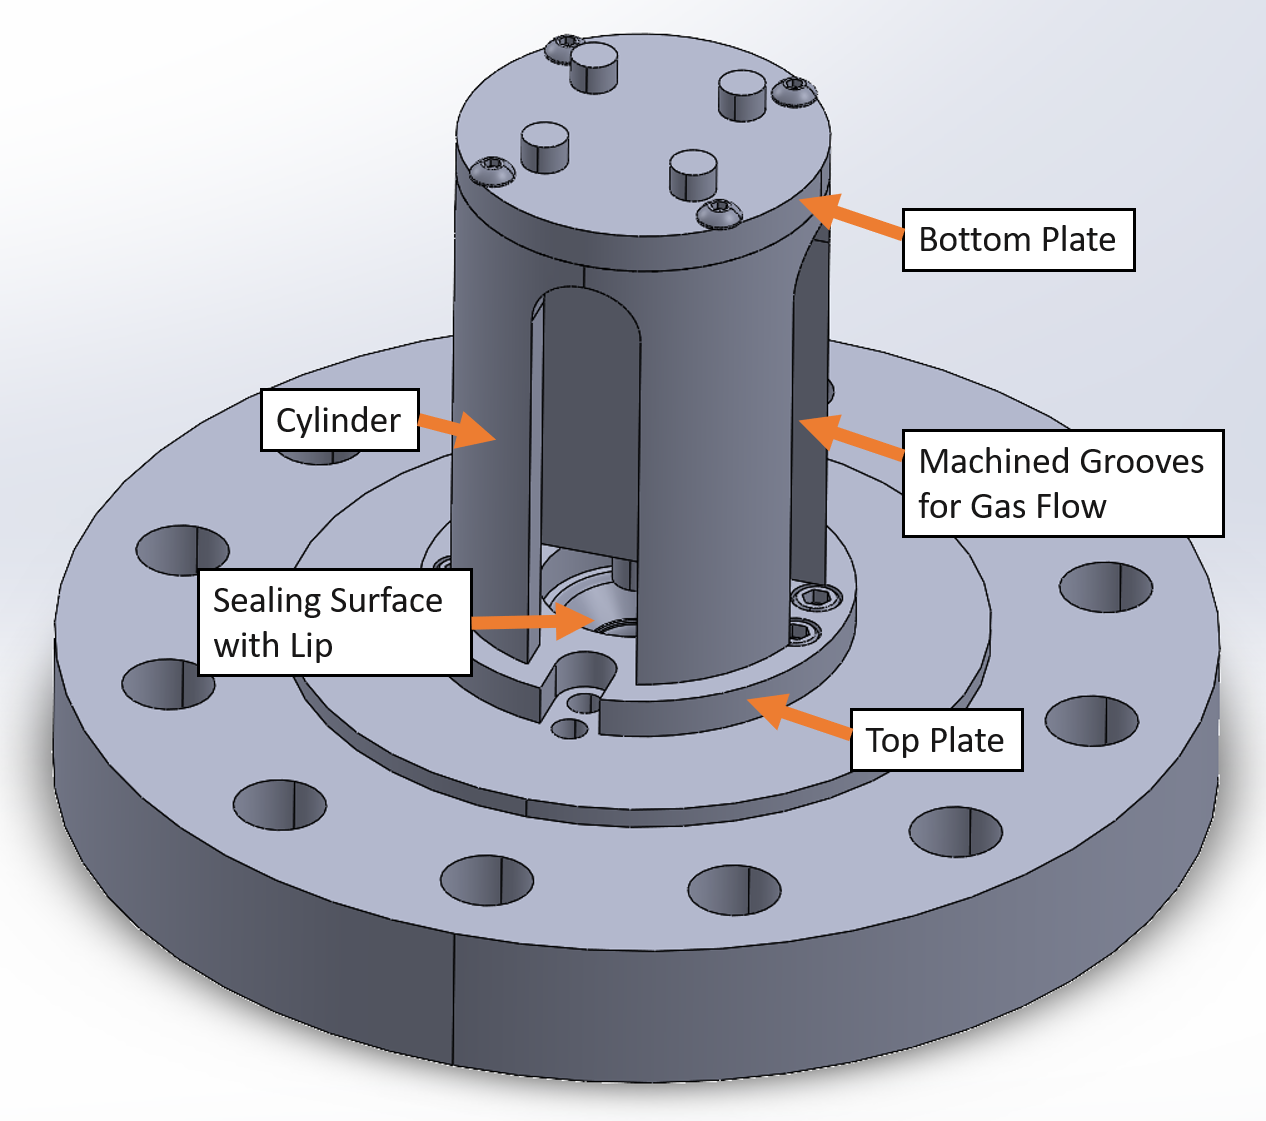
\includegraphics[width=0.88\textwidth]{design/photos/piston_mount_gen2_cad_labels.png}
        \caption{CAD model of cylindrical piston mount on flange.}
        \label{fig:cad mount 2}
    \end{subfigure}
    \hfill
    \begin{subfigure}[t]{0.45\textwidth}
        \centering
        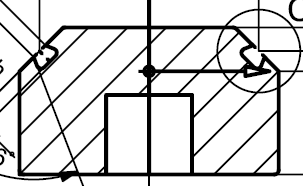
\includegraphics[width=0.66\textwidth]{design/photos/new_plug_draw_crop.PNG}
        \caption{Drawing of new plug design for piston valve with dovetail groove for an o-ring.}
        \label{fig:plug v2 draw}
    \end{subfigure}
    
    \caption{Redesigned piston valve mount and plug.}
    \label{fig:redesign}
\end{figure}

%%%%%%%%%%%%%%%%%%%%%%%%%%%%%%%%%%%%%%%%%%%%%%%%%%%%%%%%%%%%%%%%%%%%%%%%%%%%%%%%%%
% subsection about new piston compared to rupture disk
\subsection{Improved Piston Valve Compared to Rupture Disk} \label{ss:new piston v disk}
Since a new piston mount and plug have been designed, the new setup needs to be tested and compared to the rupture disk results to ensure the valve is performing adequately and the desired pressure of \SI{1.72}{\mega\pascal} (250 psi) in less than \SI{5}{\milli\second} is still reached. \Cref{fig:disk new} shows a rupture disk and a piston valve test both starting at \SI{6.9}{\mega\pascal} (1000 psi), with a \SI{2.54}{\centi\meter} (1 inch) inner diameter intermediate section. The pressure evolution of the piston valve follows very closely to the rupture disk and the desired pressurization is reached. \Cref{fig:piston 1000psi 25ms} shows a piston valve test under the same conditions, but has more instrumentation included. Comparing this plot to \Cref{fig:disk} shows that the piston valve produces pressure and density waves very similar to those of the rupture disk. Therefore, the repeatability of the improved piston mount and plug can be tested. 

\begin{figure}[htbp]
    \vspace{16pt}
    \centering
    \begin{subfigure}[t]{0.45\textwidth}
        \centering
        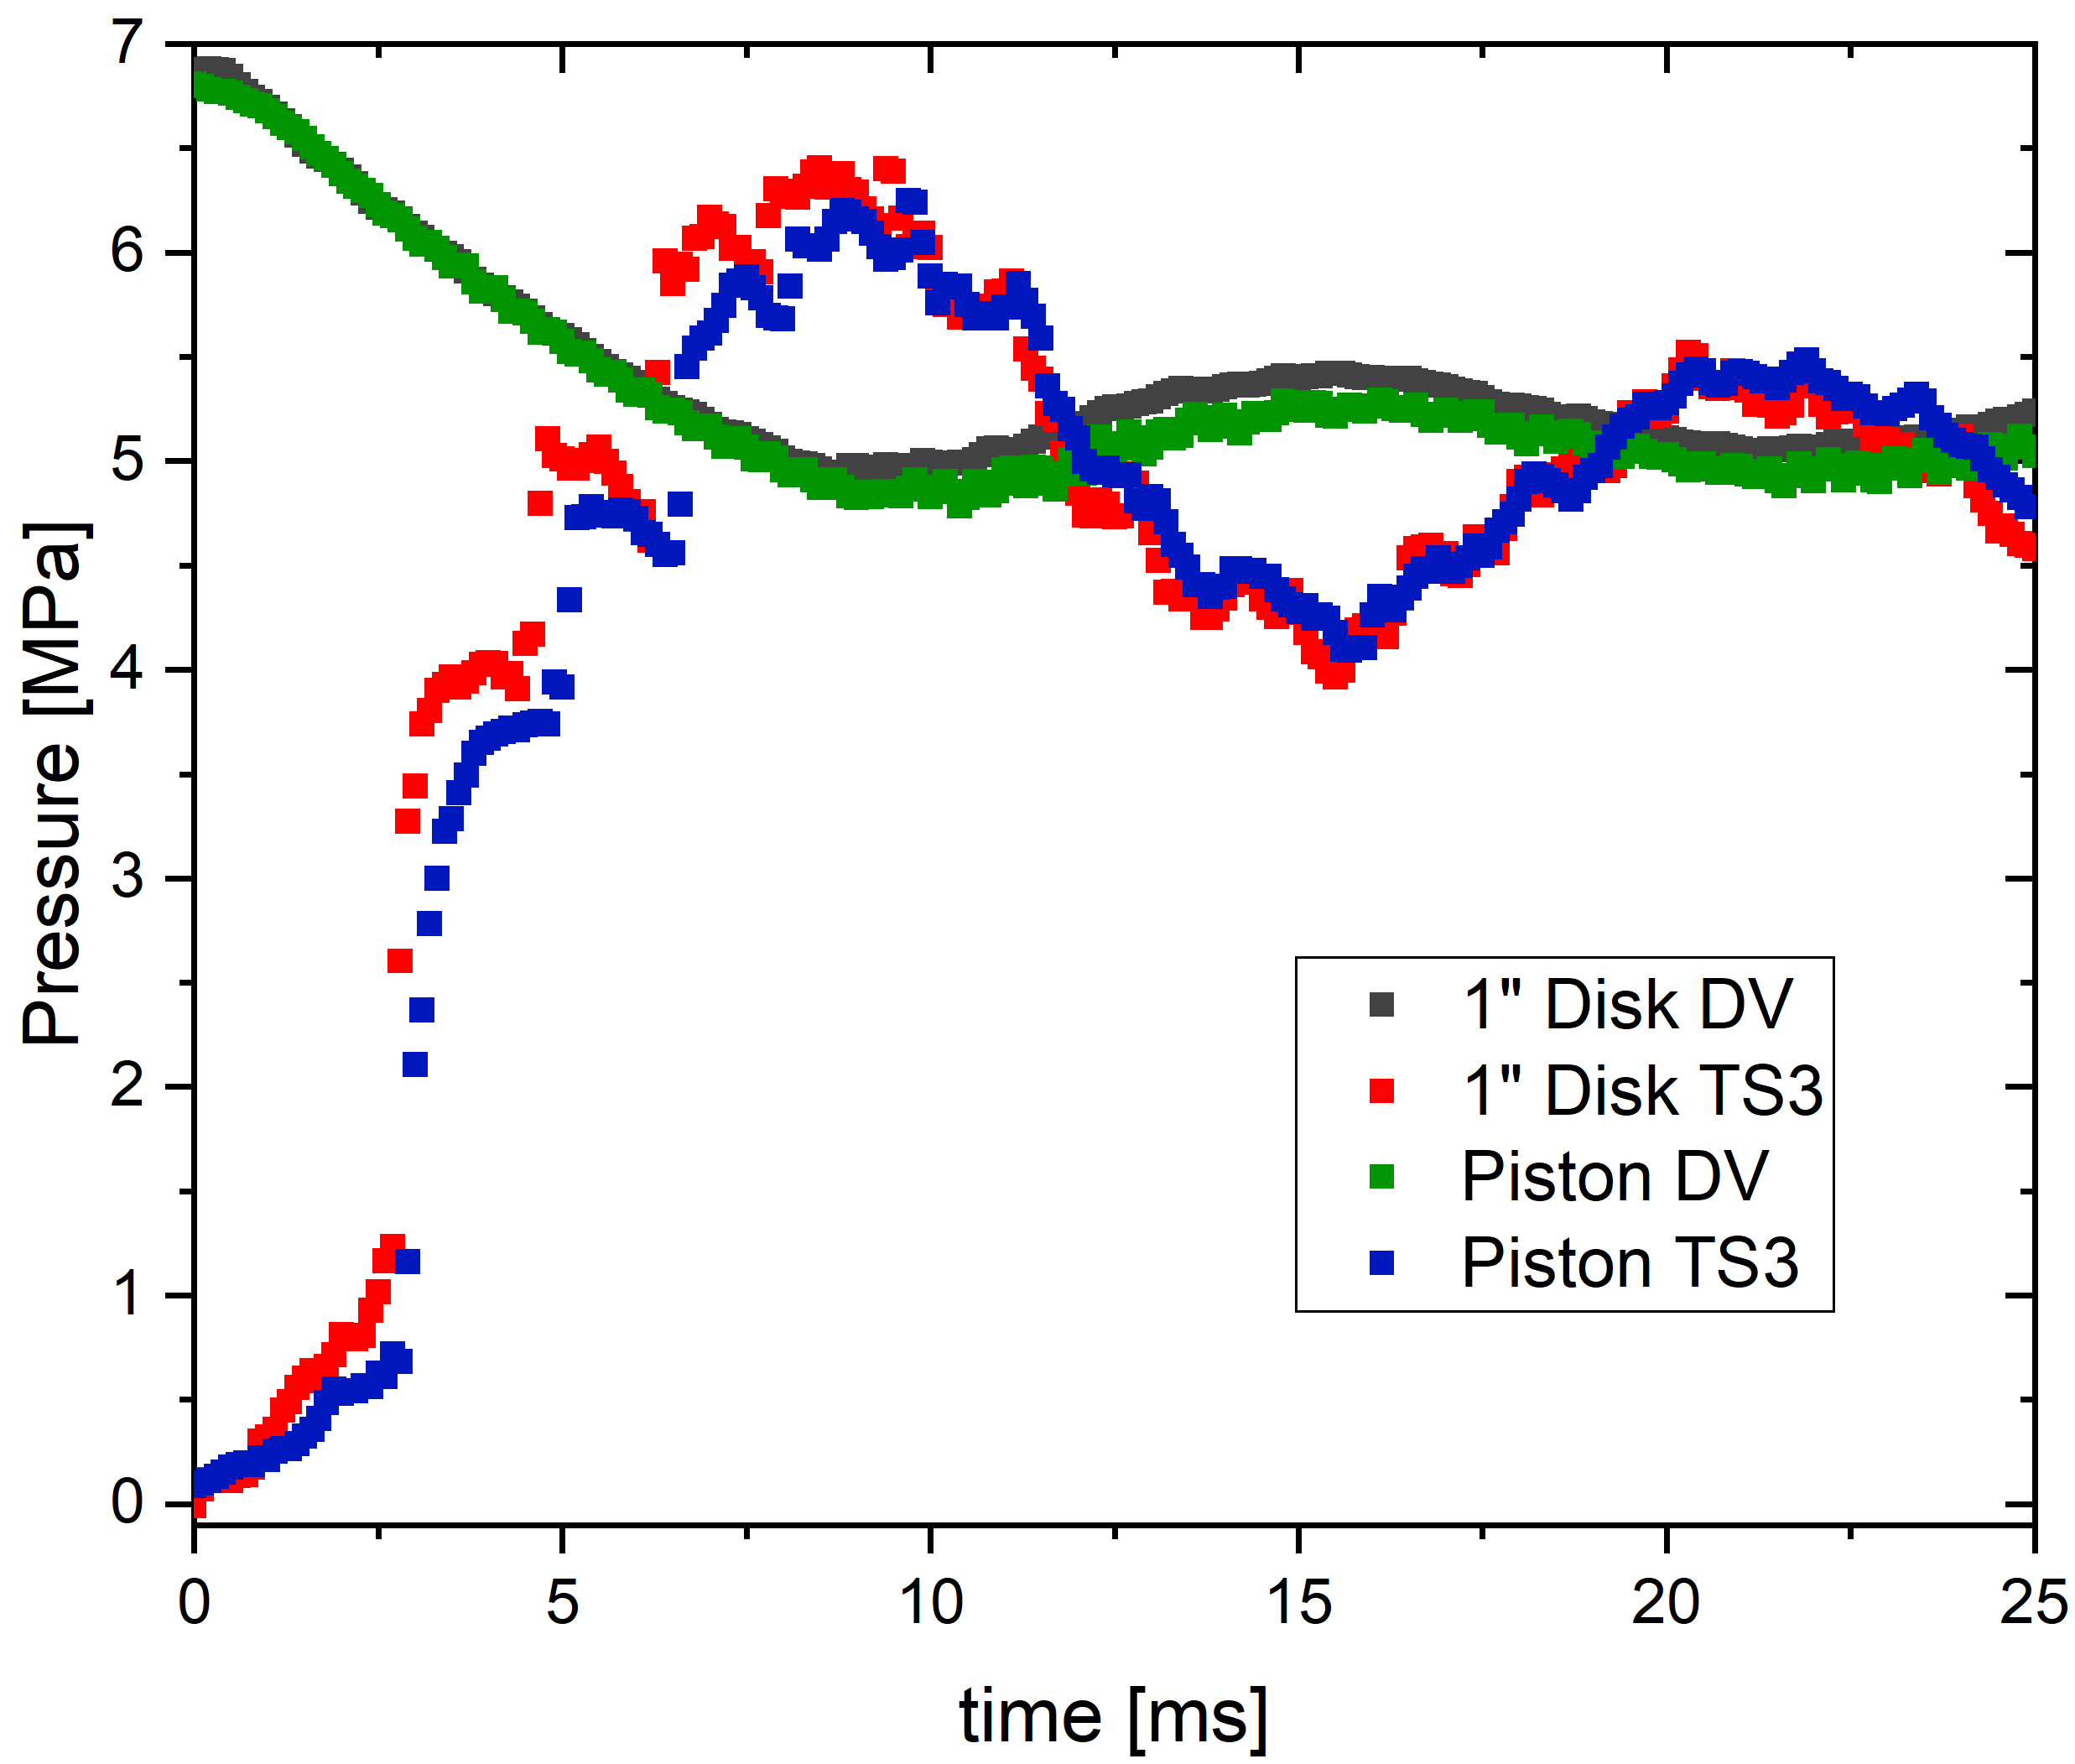
\includegraphics[width=0.9\textwidth]{results/plots/BD_Piston_1000_overlay.png}
        \caption{Pressure over time for rupture disk compared to the second generation plug design HENRI test.}
        \label{fig:disk new}
    \end{subfigure}
    \hfill
    \begin{subfigure}[t]{0.45\textwidth}
        \centering
        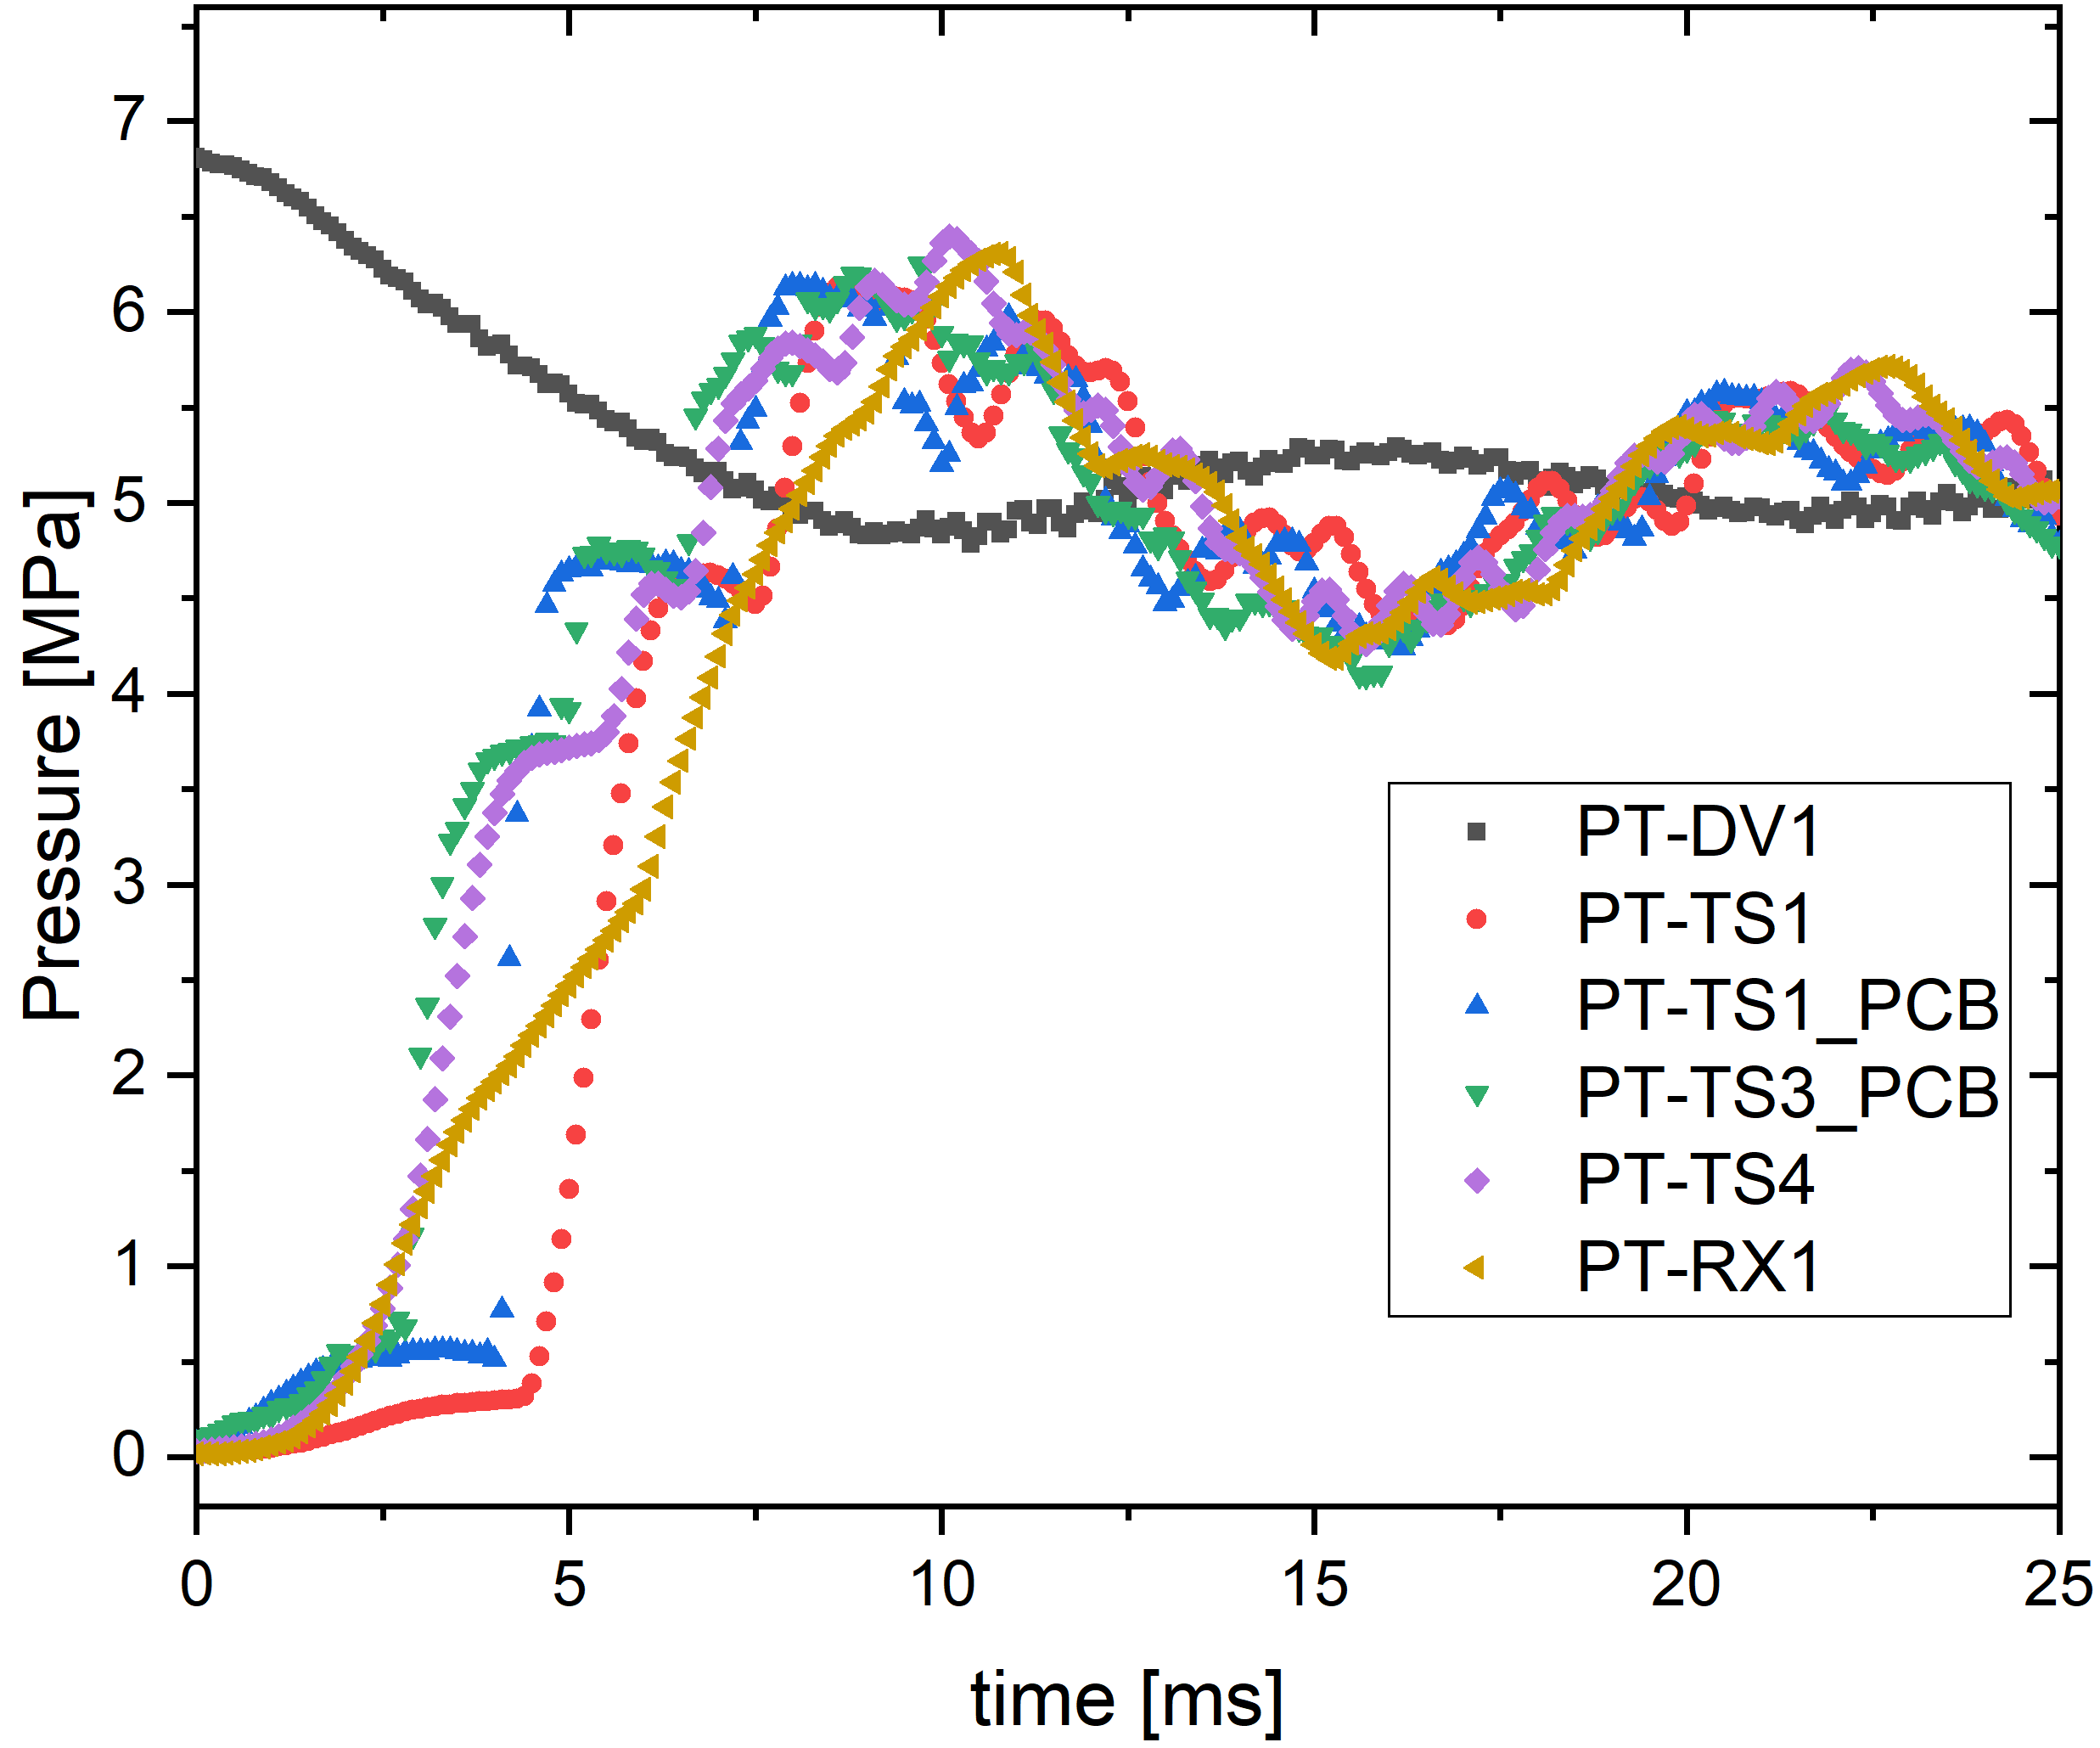
\includegraphics[width=0.9\textwidth]{results/plots/1000psi_Mpa_25.png}
        \caption{Pressure over time for a test using a FFKM o-ring on the second generation plug design.}
        \label{fig:piston 1000psi 25ms}
    \end{subfigure}
    
    \caption{Comparison of rupture disk and improved piston valve HENRI tests at an initial pressure of \SI{6.9}{\mega\pascal} (\SI{1000}{psia}) and with intermediate tube inner diameter of \SI{2.54}{\centi\meter} (\SI{1}{inch}).}
    \label{fig:new piston v disk}
    \vspace{16pt}
\end{figure}


%%%%%%%%%%%%%%%%%%%%%%%%%%%%%%%%%%%%%%%%%%%%%%%%%%%%%%%%%%%%%%%%%%%%%%%%%%%%%%%%%%
% subsection about new piston valve repeatability
\subsection{Improved Piston Valve Repeatability} \label{ss:new repeatability}
The repeatability is tested in the same manner as the first piston valve design. The piston valve is tested at the same initial pressure to determine the repeatability and consistency, then the valve is tested at varying initial pressures to provide data to predict the valve's operation and pressure evolution over a range of pressures. \Cref{fig:new piston 2 test} shows two tests at an initial pressure of \SI{6.9}{\mega\pascal} (1000 psi). The two tests overlap each other well and demonstrate the piston valve can produce the same pressurization in the HENRI cartridge for multiple tests. \Cref{fig:new norm} presents tests over a range of initial pressures, normalized by the initial pressure. The highest three initial pressures provide very similar results, that also match well with the rupture disk tests. However, \SI{2.5}{\mega\pascal} (360 psi) and lower deviate and pressurize slower, with less oscillation. The behavior of the valve and HENRI cartridge at low initial pressure is useful to know so TREAT has more flexibility in transient capability. The improved piston valve design also can seal at much lower pressures than the metal only plug design, which further increases the capability of the system.

\begin{figure}[htbp]
    \centering
    \begin{subfigure}[t]{0.45\textwidth}
        \centering
        %\includegraphics[width=0.9\textwidth]{}
        \caption{Comparison of two improved piston valve tests at an initial pressure of \SI{6.9}{\mega\pascal} (1000 psi).}
        \label{fig:new piston 2 test}
    \end{subfigure}
    \hfill
    \begin{subfigure}[t]{0.45\textwidth}
        \centering
        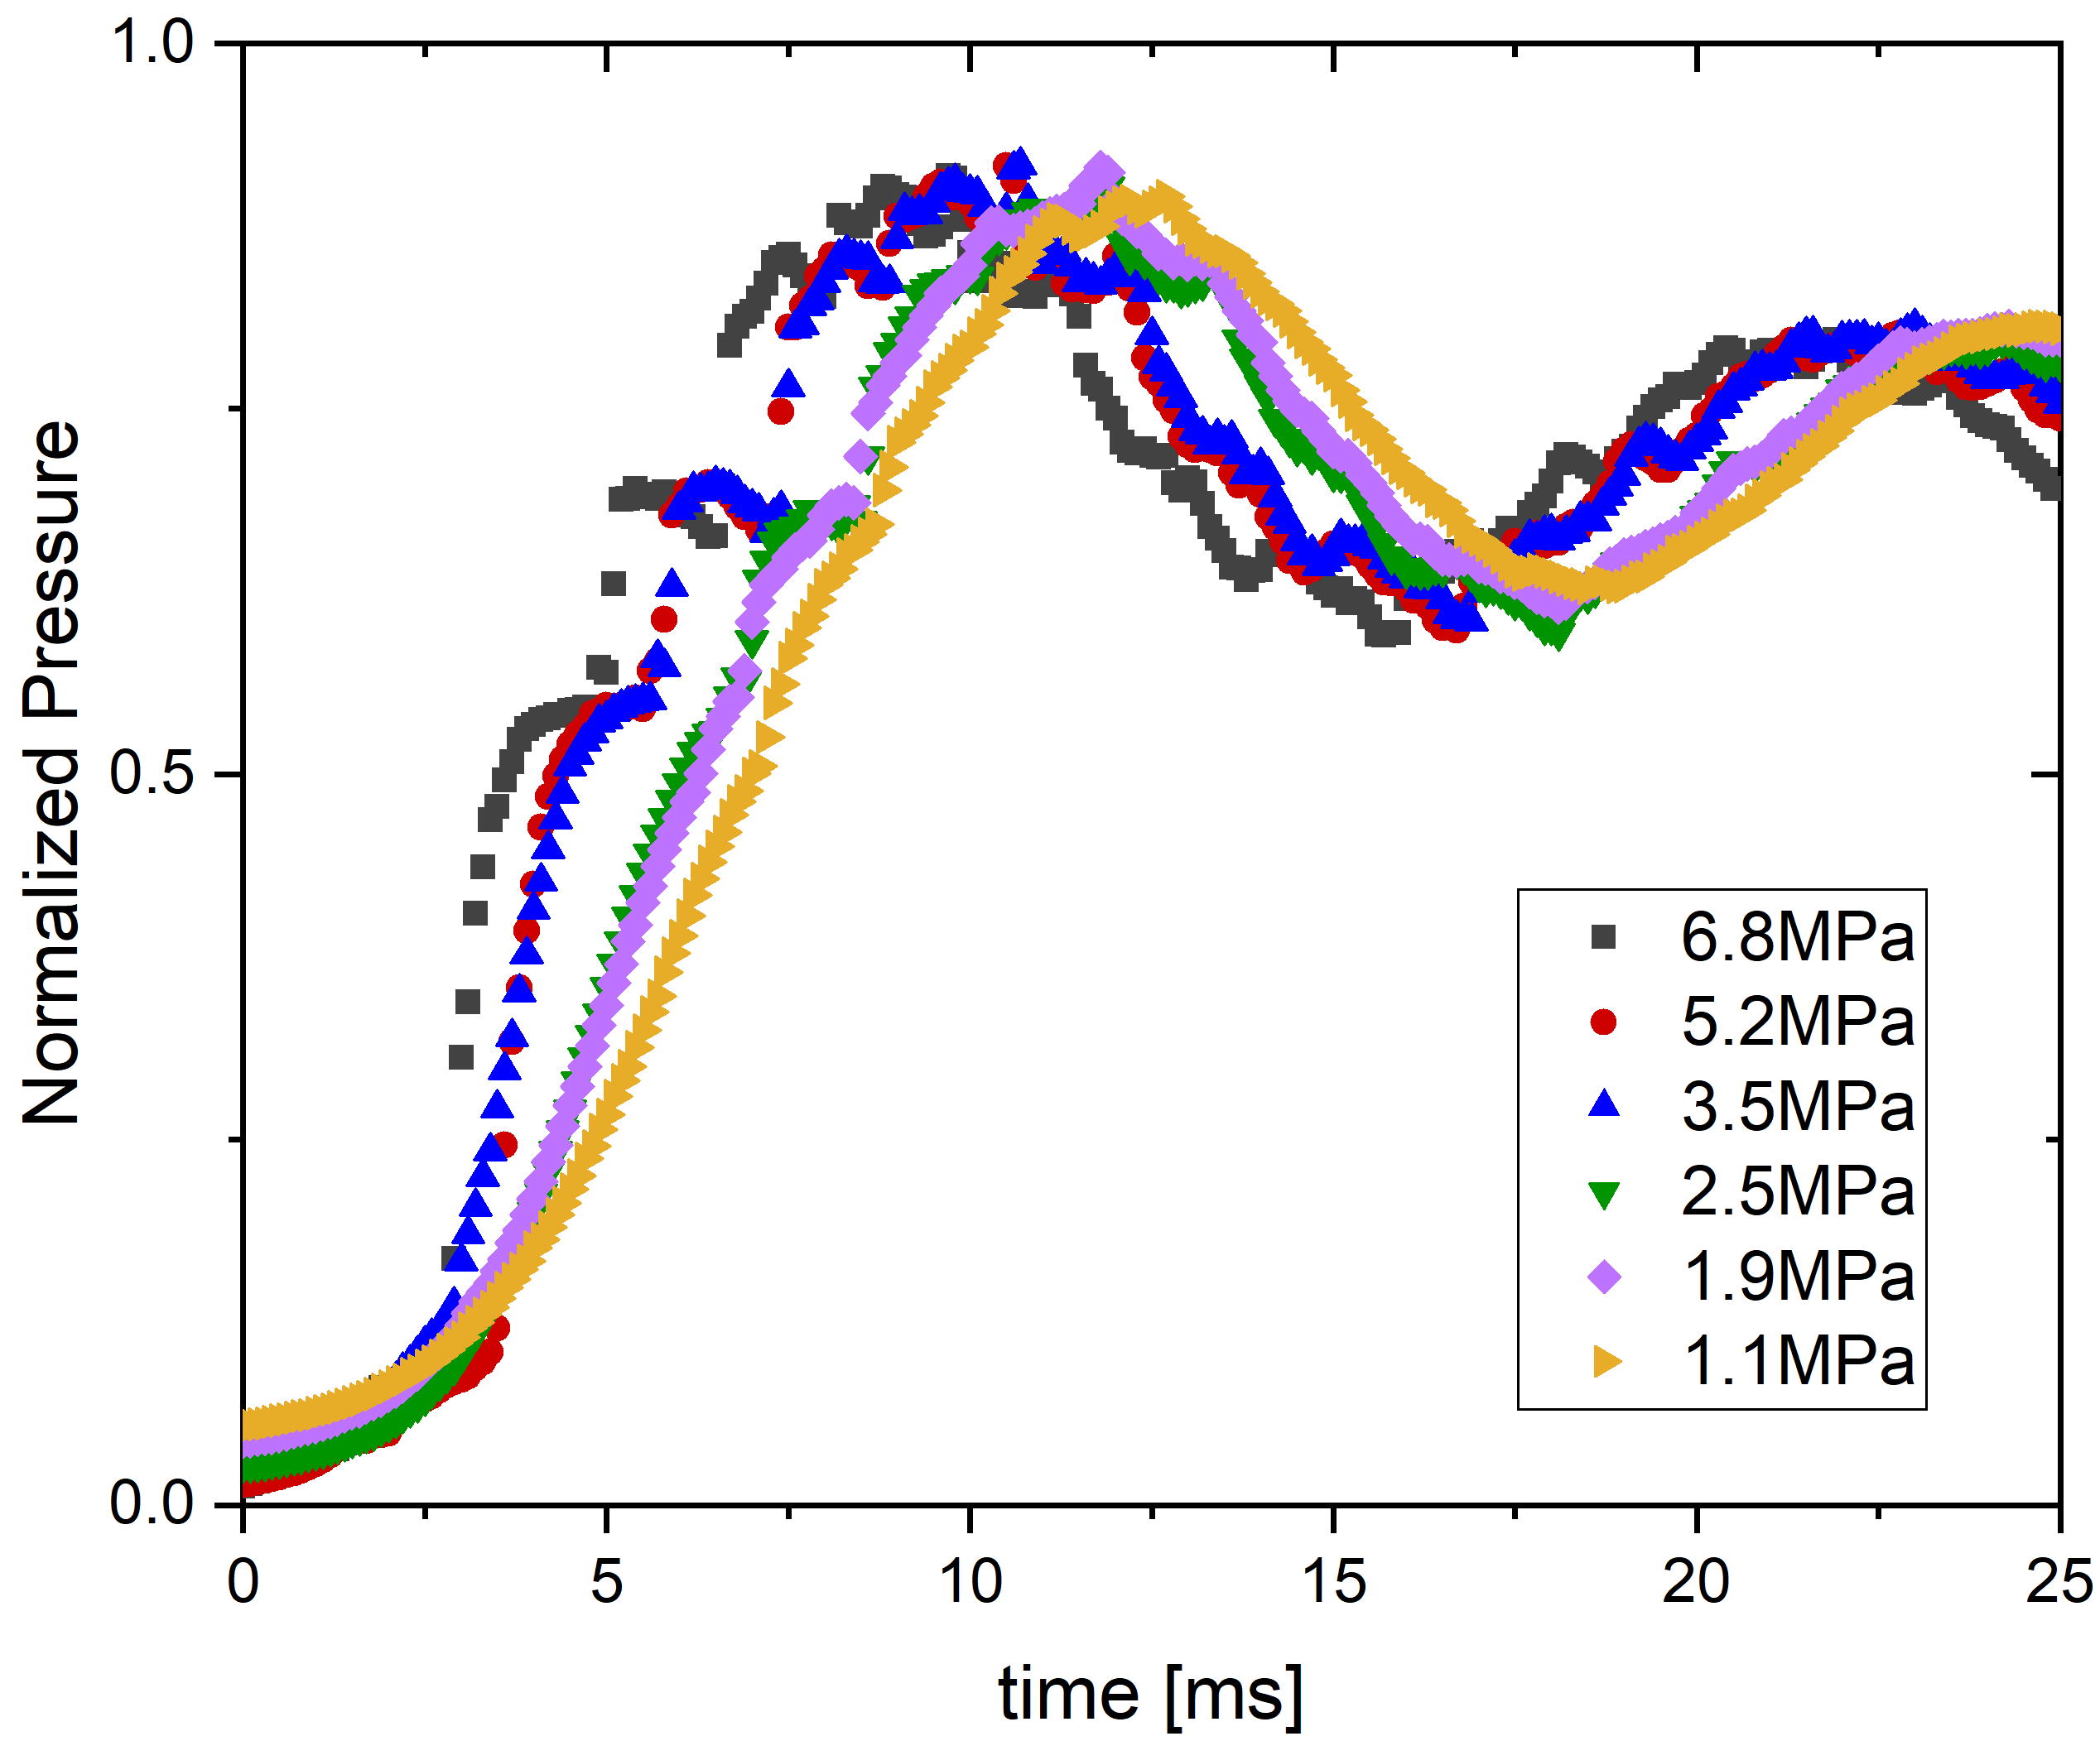
\includegraphics[width=0.9\textwidth]{results/plots/norm_FFKM.png}
        \caption{Improved piston valve test results, at position TS3, normalized by initial driver tank pressure for a range of initial driver tank pressures.}
        \label{fig:new norm}
    \end{subfigure}
    \caption{Comparison of results for improved piston valve to demonstrate repeatability at one initial pressure and predictability at varying initial pressures.}
    \label{fig:new piston repeatability}
\end{figure}

%%%%%%%%%%%%%%%%%%%%%%%%%%%%%%%%%%%%%%%%%%%%%%%%%%%%%%%%%%%%%%%%%%%%%%%%%%%%%%%%%%
% subsection about new piston valve reusability
\subsection{Improved Piston Valve Re-usability} \label{ss:new reusability}

% subsection comparing metal-to-metal seal and o-ring plugs
% \subsection{Metal-to-Metal Plug Compared to O-ring Plug}
% The metal-to-metal plug design did not seal as well as the o-ring design, which led to a leak from the driver tank into the test section before the piston valve opened all the way. The o-ring plug does not have this issue, even at low operating pressures (below \SI{1.72}{\mega\pascal} (\SI{250}{psi})). \Cref{fig:metal vs oring} shows a test using each plug type. The pressure at [INSERT CORRECT POSITION HERE (probably TS1)] for the metal-to-metal seal increases slightly before the other positions, and before the driver tank pressure decreases significantly, showing that with only the pressure of the driver tank holding it closed, the metal-to-metal seal does not work well. In contrast, the o-ring plug is able to maintain the pressure boundary until the valve opens fully, which provides a quick, crisp helium injection.

% \begin{figure}
%     \vspace{16pt}
%     \centering
%     %\includegraphics{}
%     \caption{Results of tests with an initial pressure of [PRESSURE] for the metal-to-metal plug and the o-ring plug.}
%     \label{fig:metal vs oring}
%     \vspace{16pt}
% \end{figure}



% \begin{figure}[htbp]
%     \vspace{16pt}
%     \centering
%     \begin{subfigure}{0.32\textwidth}
%         \centering
%         \includegraphics[width=\textwidth]{results/plots/270psi_MPa_25.png}
%         \caption{\SI{1724}{\kilo\pascal} (\SI{250}{psi})}
%         \label{fig:piston multi 250}
%     \end{subfigure}
%     \hfill
%     \begin{subfigure}{0.32\textwidth}
%         \centering
%         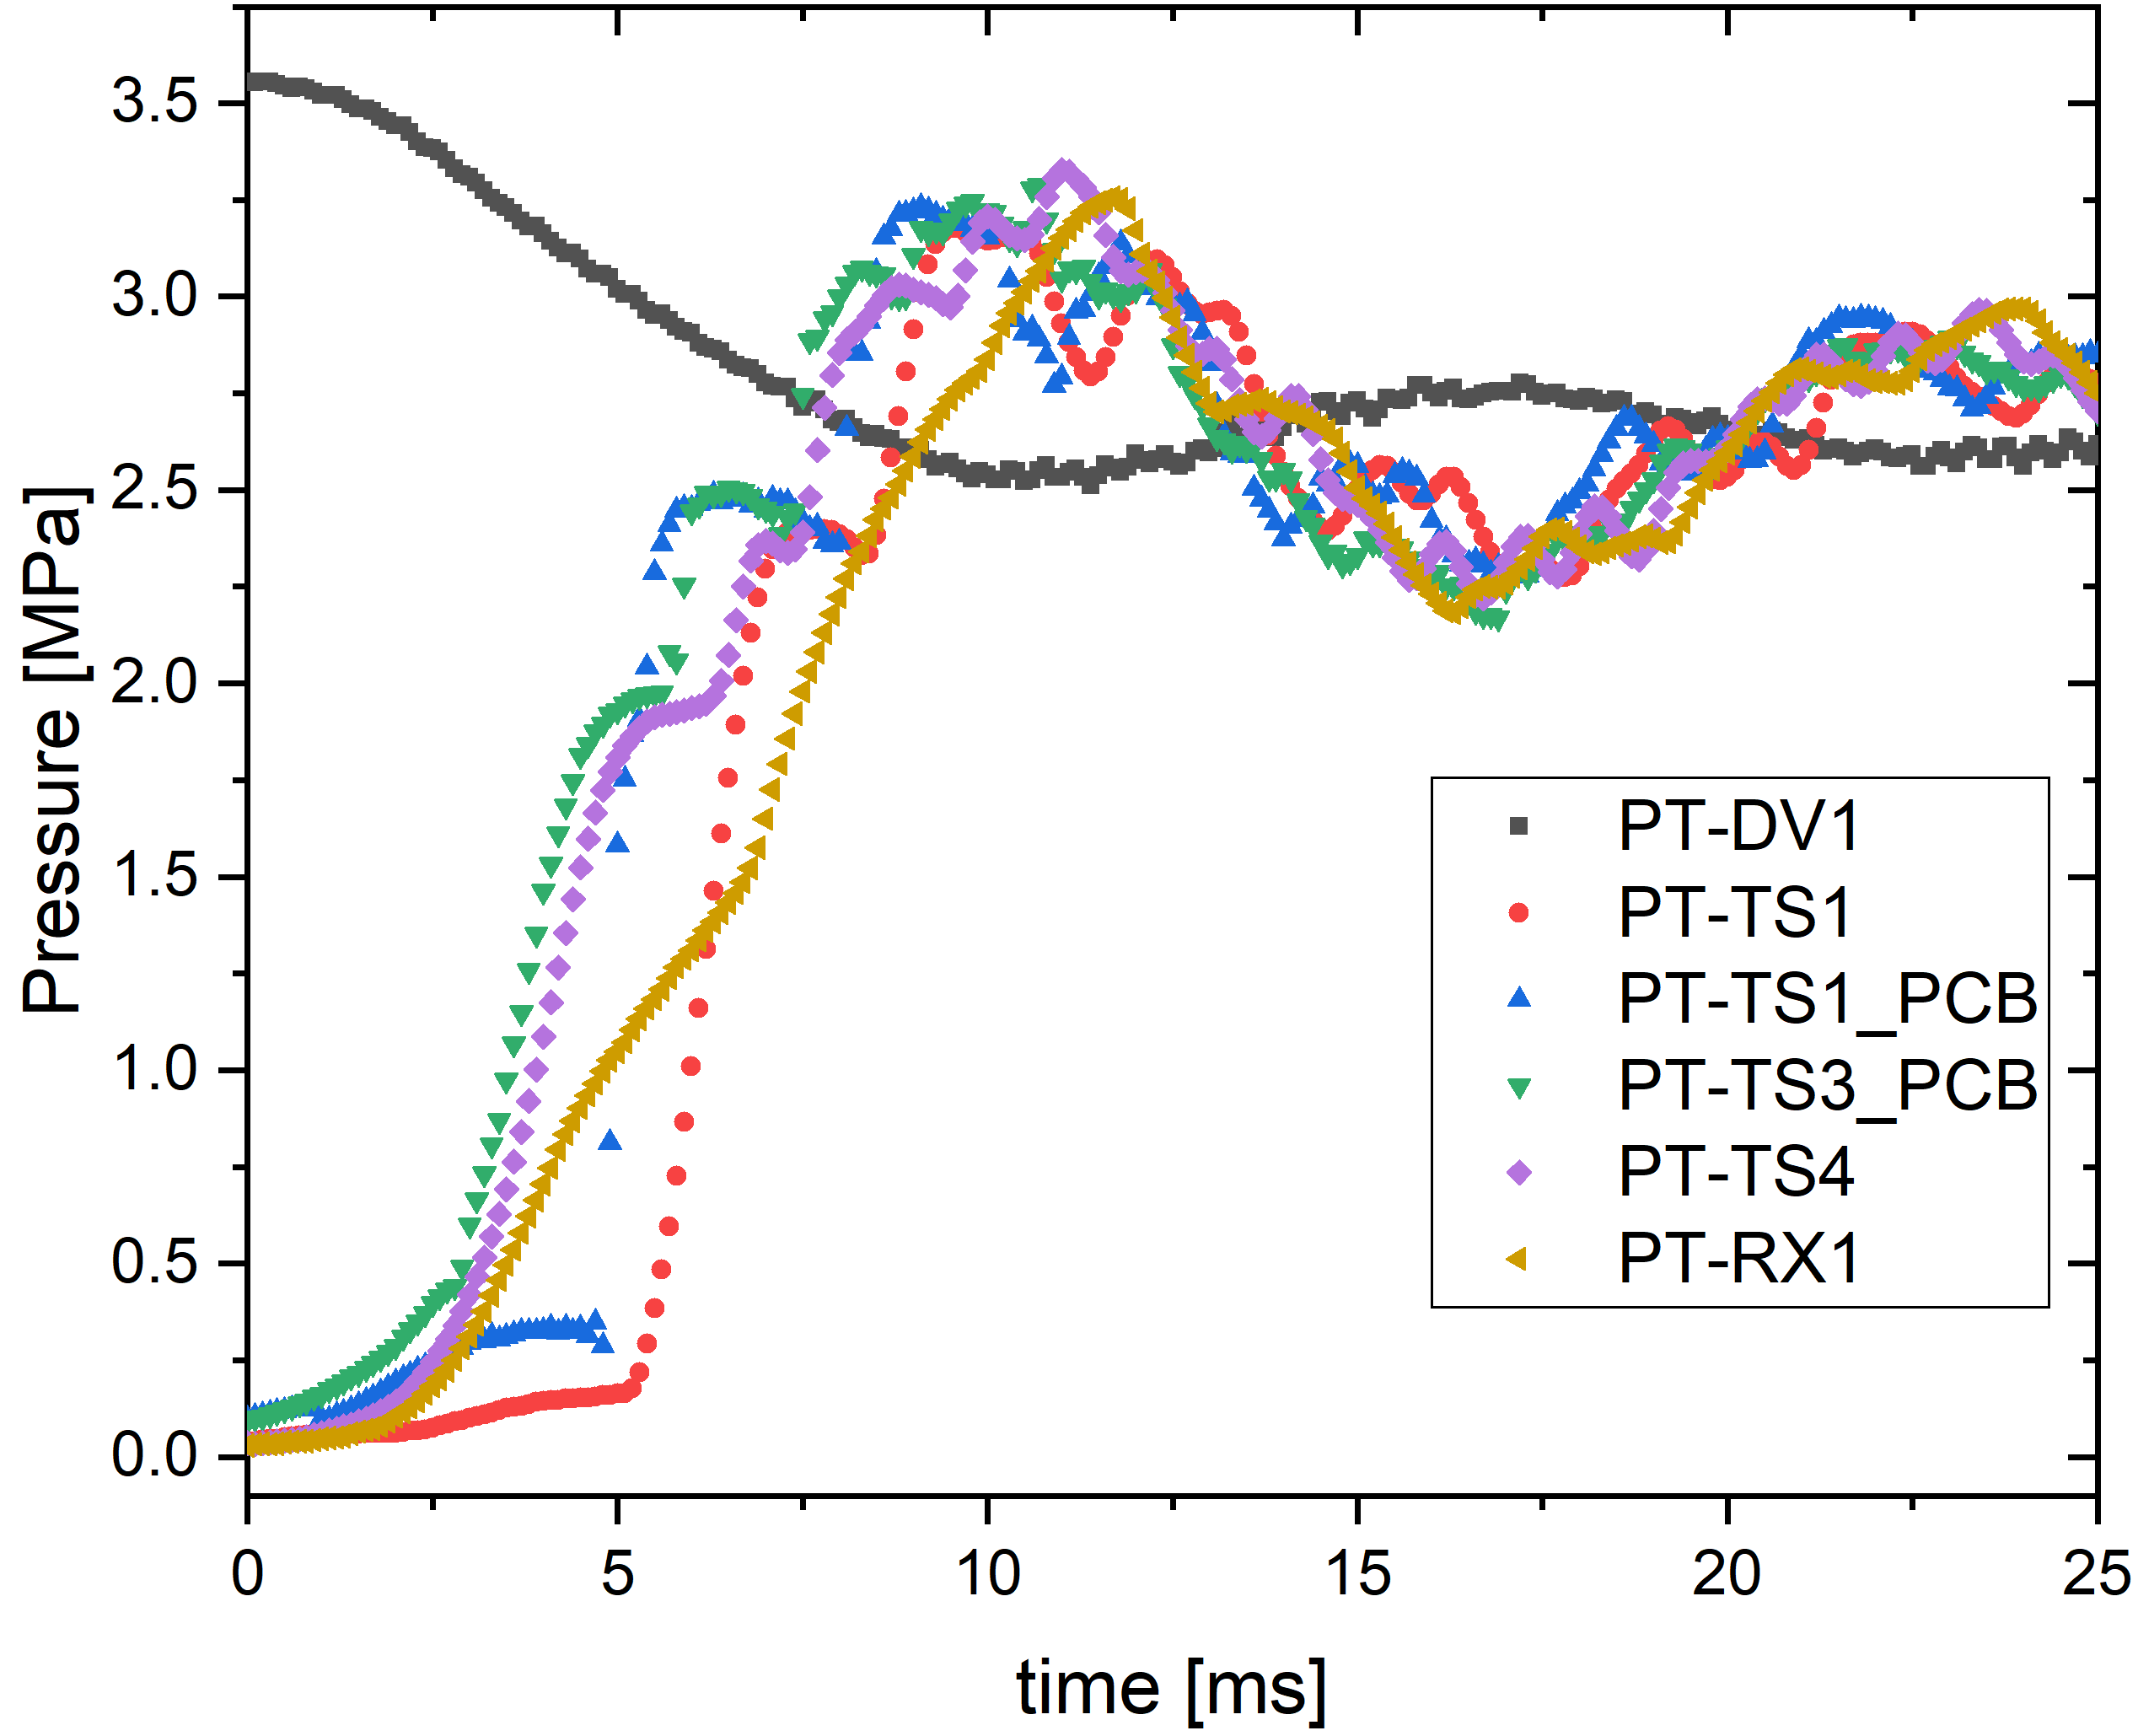
\includegraphics[width=\textwidth]{results/plots/500psi_Mpa_25.png}
%         \caption{\SI{3448}{\kilo\pascal} (\SI{500}{psi})}
%         \label{fig:piston multi 500}
%     \end{subfigure}
%     \hfill
%     \begin{subfigure}{0.32\textwidth}
%         \centering
%         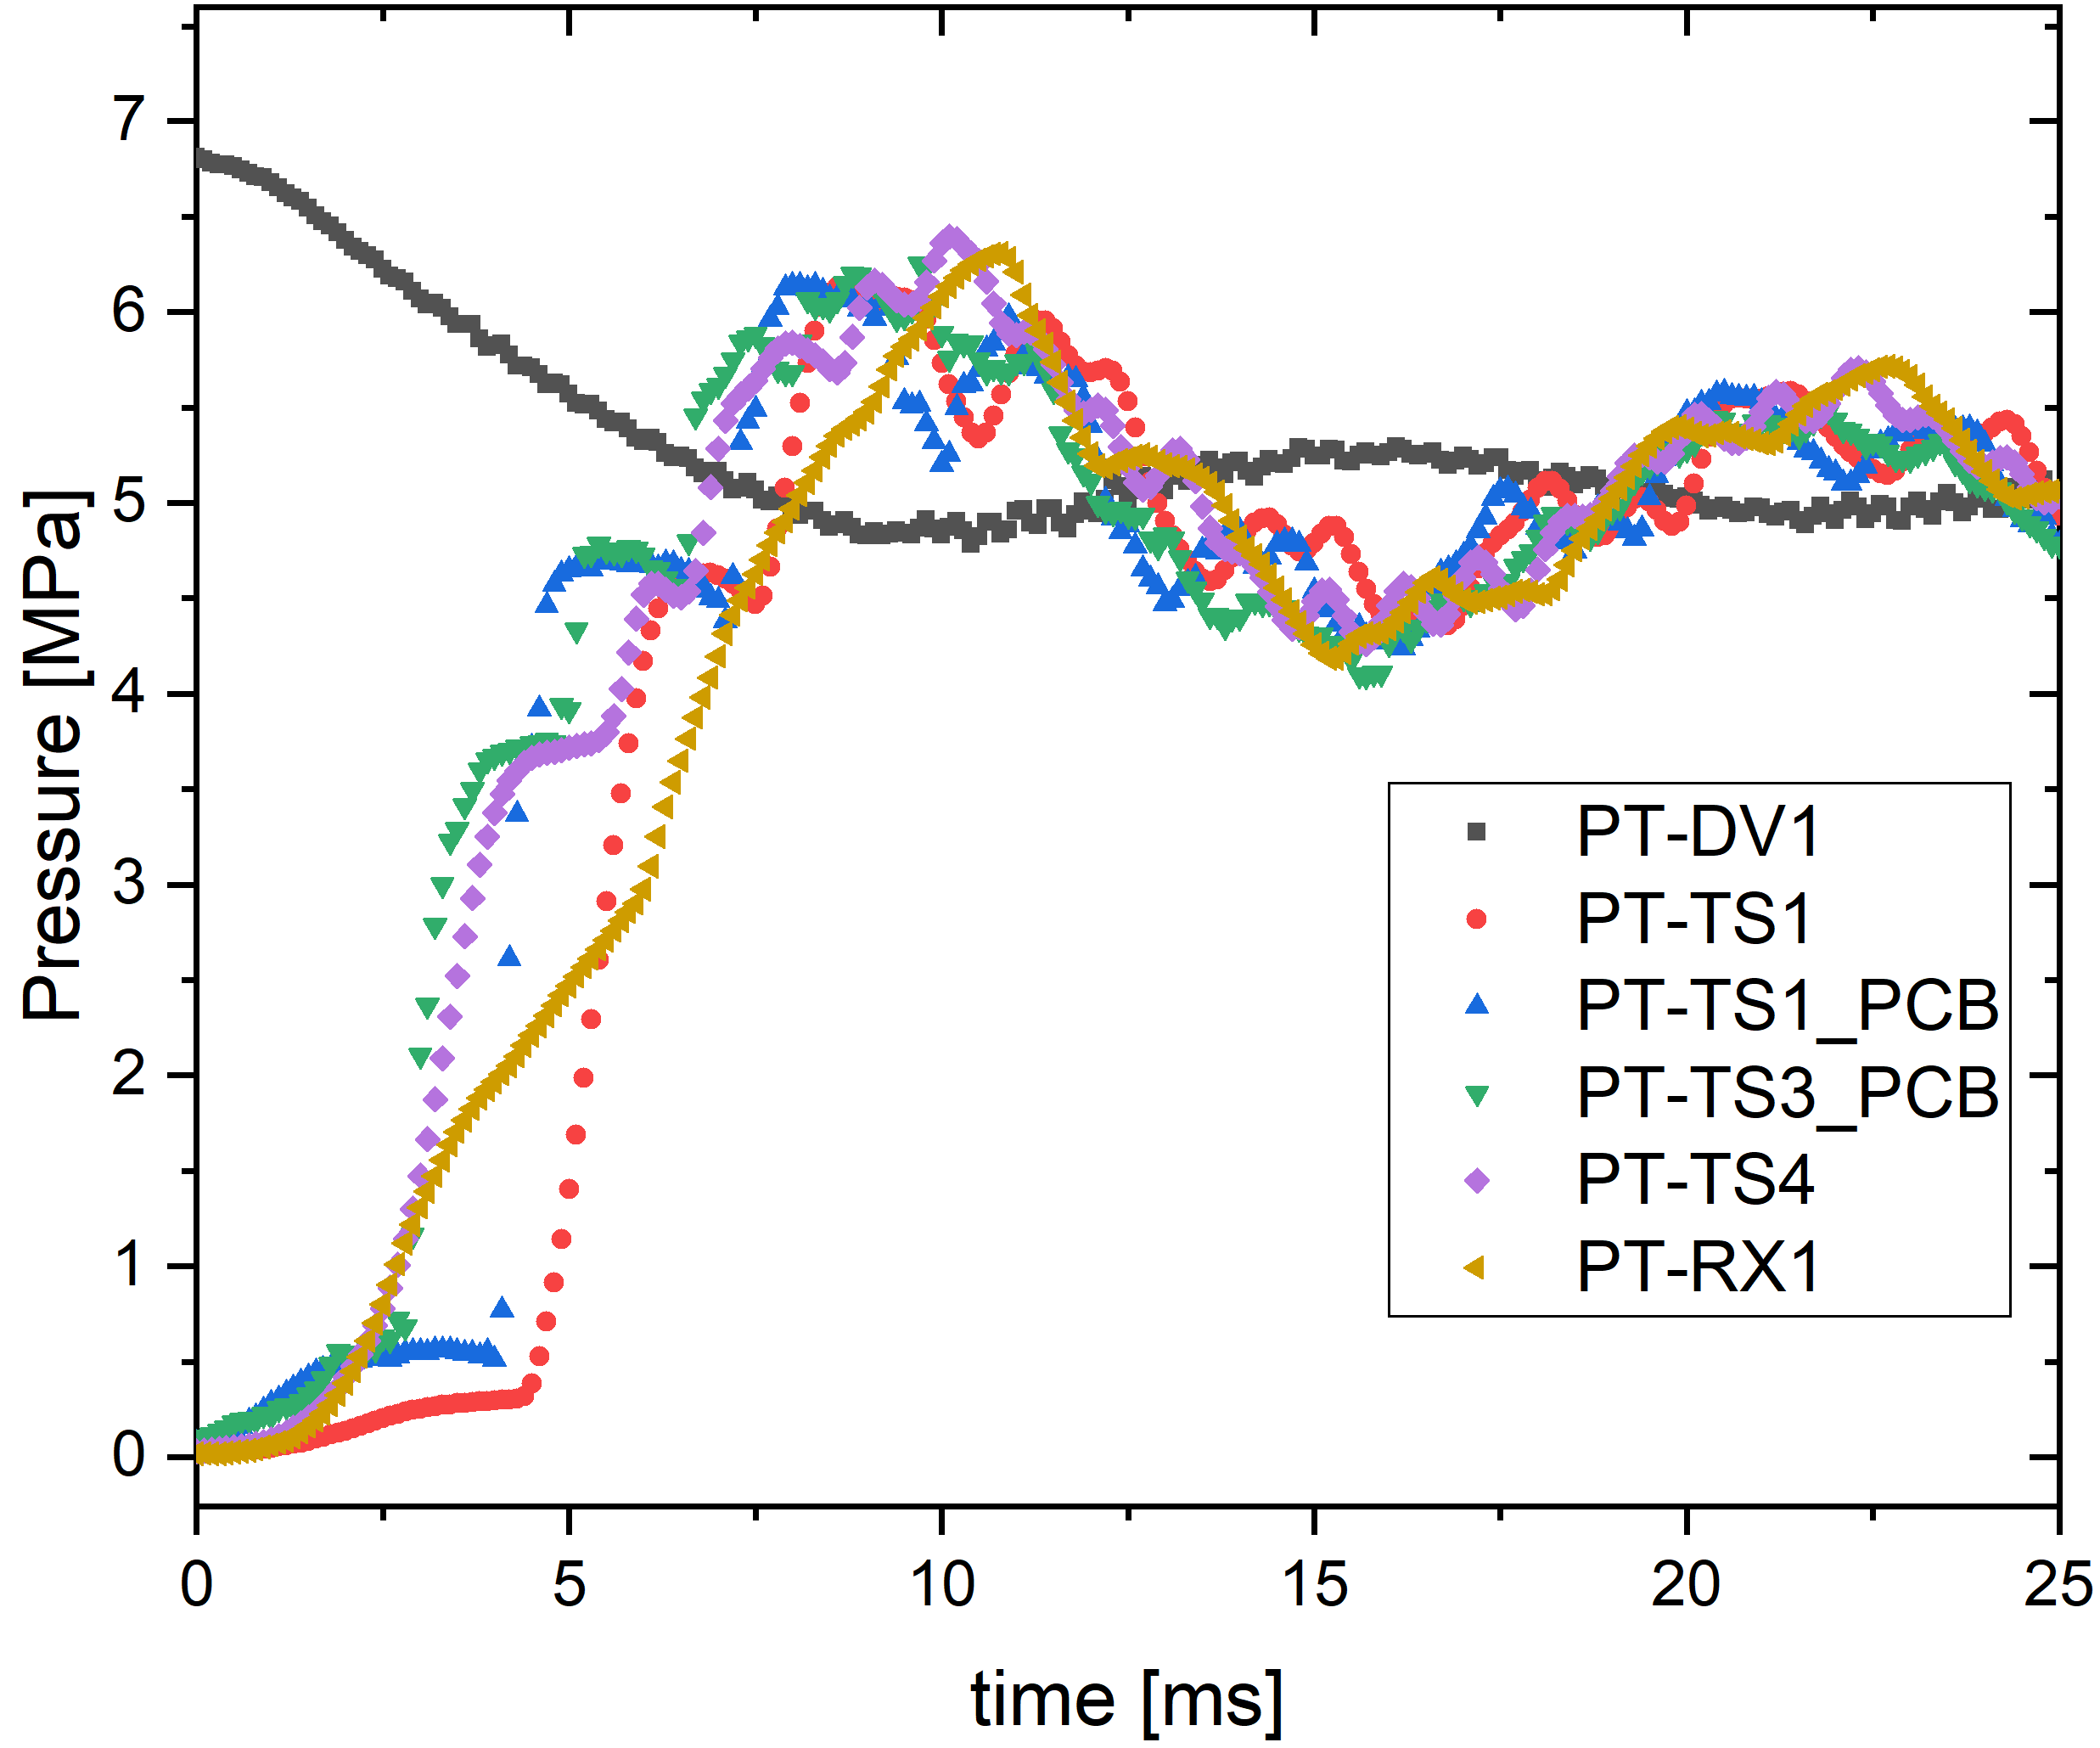
\includegraphics[width=\textwidth]{results/plots/1000psi_Mpa_25.png}
%         \caption{\SI{6896}{\kilo\pascal} (\SI{1000}{psi})}
%         \label{fig:piston multi 1000}
%     \end{subfigure}
%     %\vspace{8pt}
%     % \begin{subfigure}{0.24\textwidth}
%     %     \centering
%     %     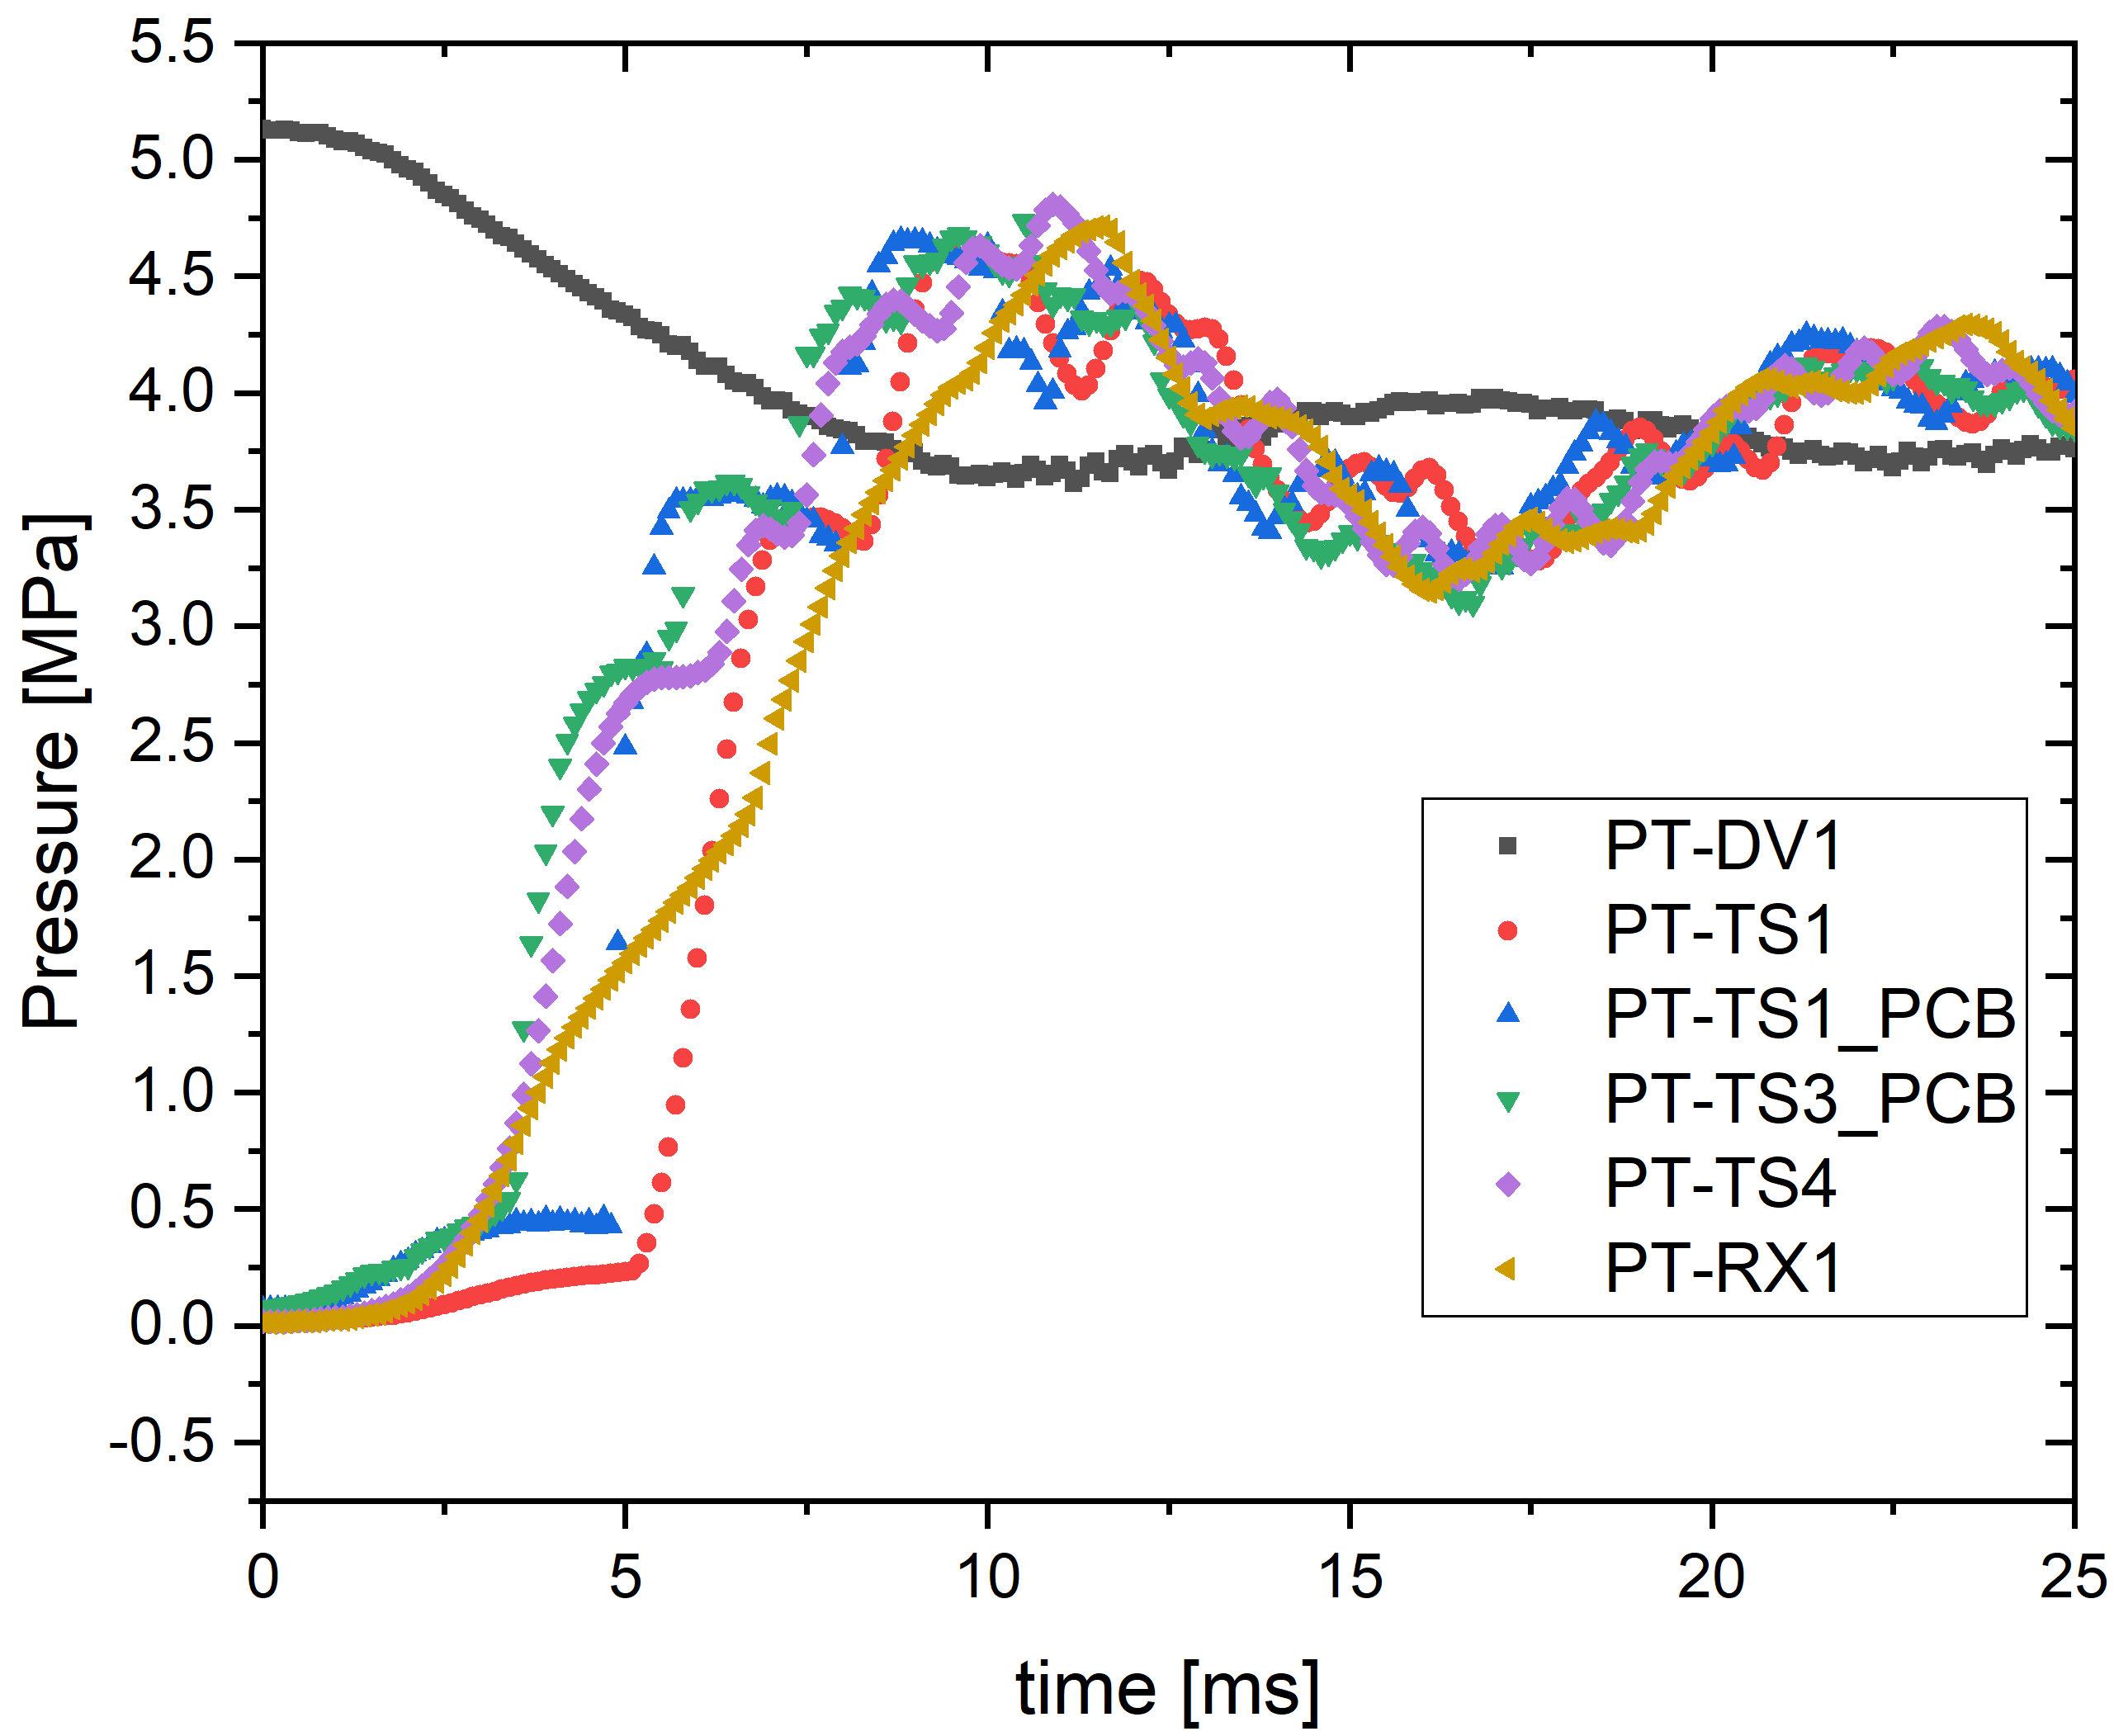
\includegraphics[width=\textwidth]{results/plots/750psi_Mpa_25.png}
%     %     \caption{\SI{5172}{\kilo\pascal} (\SI{750}{psi})}
%     %     \label{fig:piston multi 750}
%     % \end{subfigure}
%     % \hfill
    

%     \caption{Pressure evolution for HENRI tests beginning at pressures ranging from \SI{1724}{\kilo\pascal} (\SI{250}{psi}) to \SI{6896}{\kilo\pascal} (\SI{1000}{psi}).}
%     \label{fig:piston multi}
%     \vspace{16pt}
% \end{figure}




% \begin{figure}[htbp]
%     \vspace{16pt}
%     \centering
%     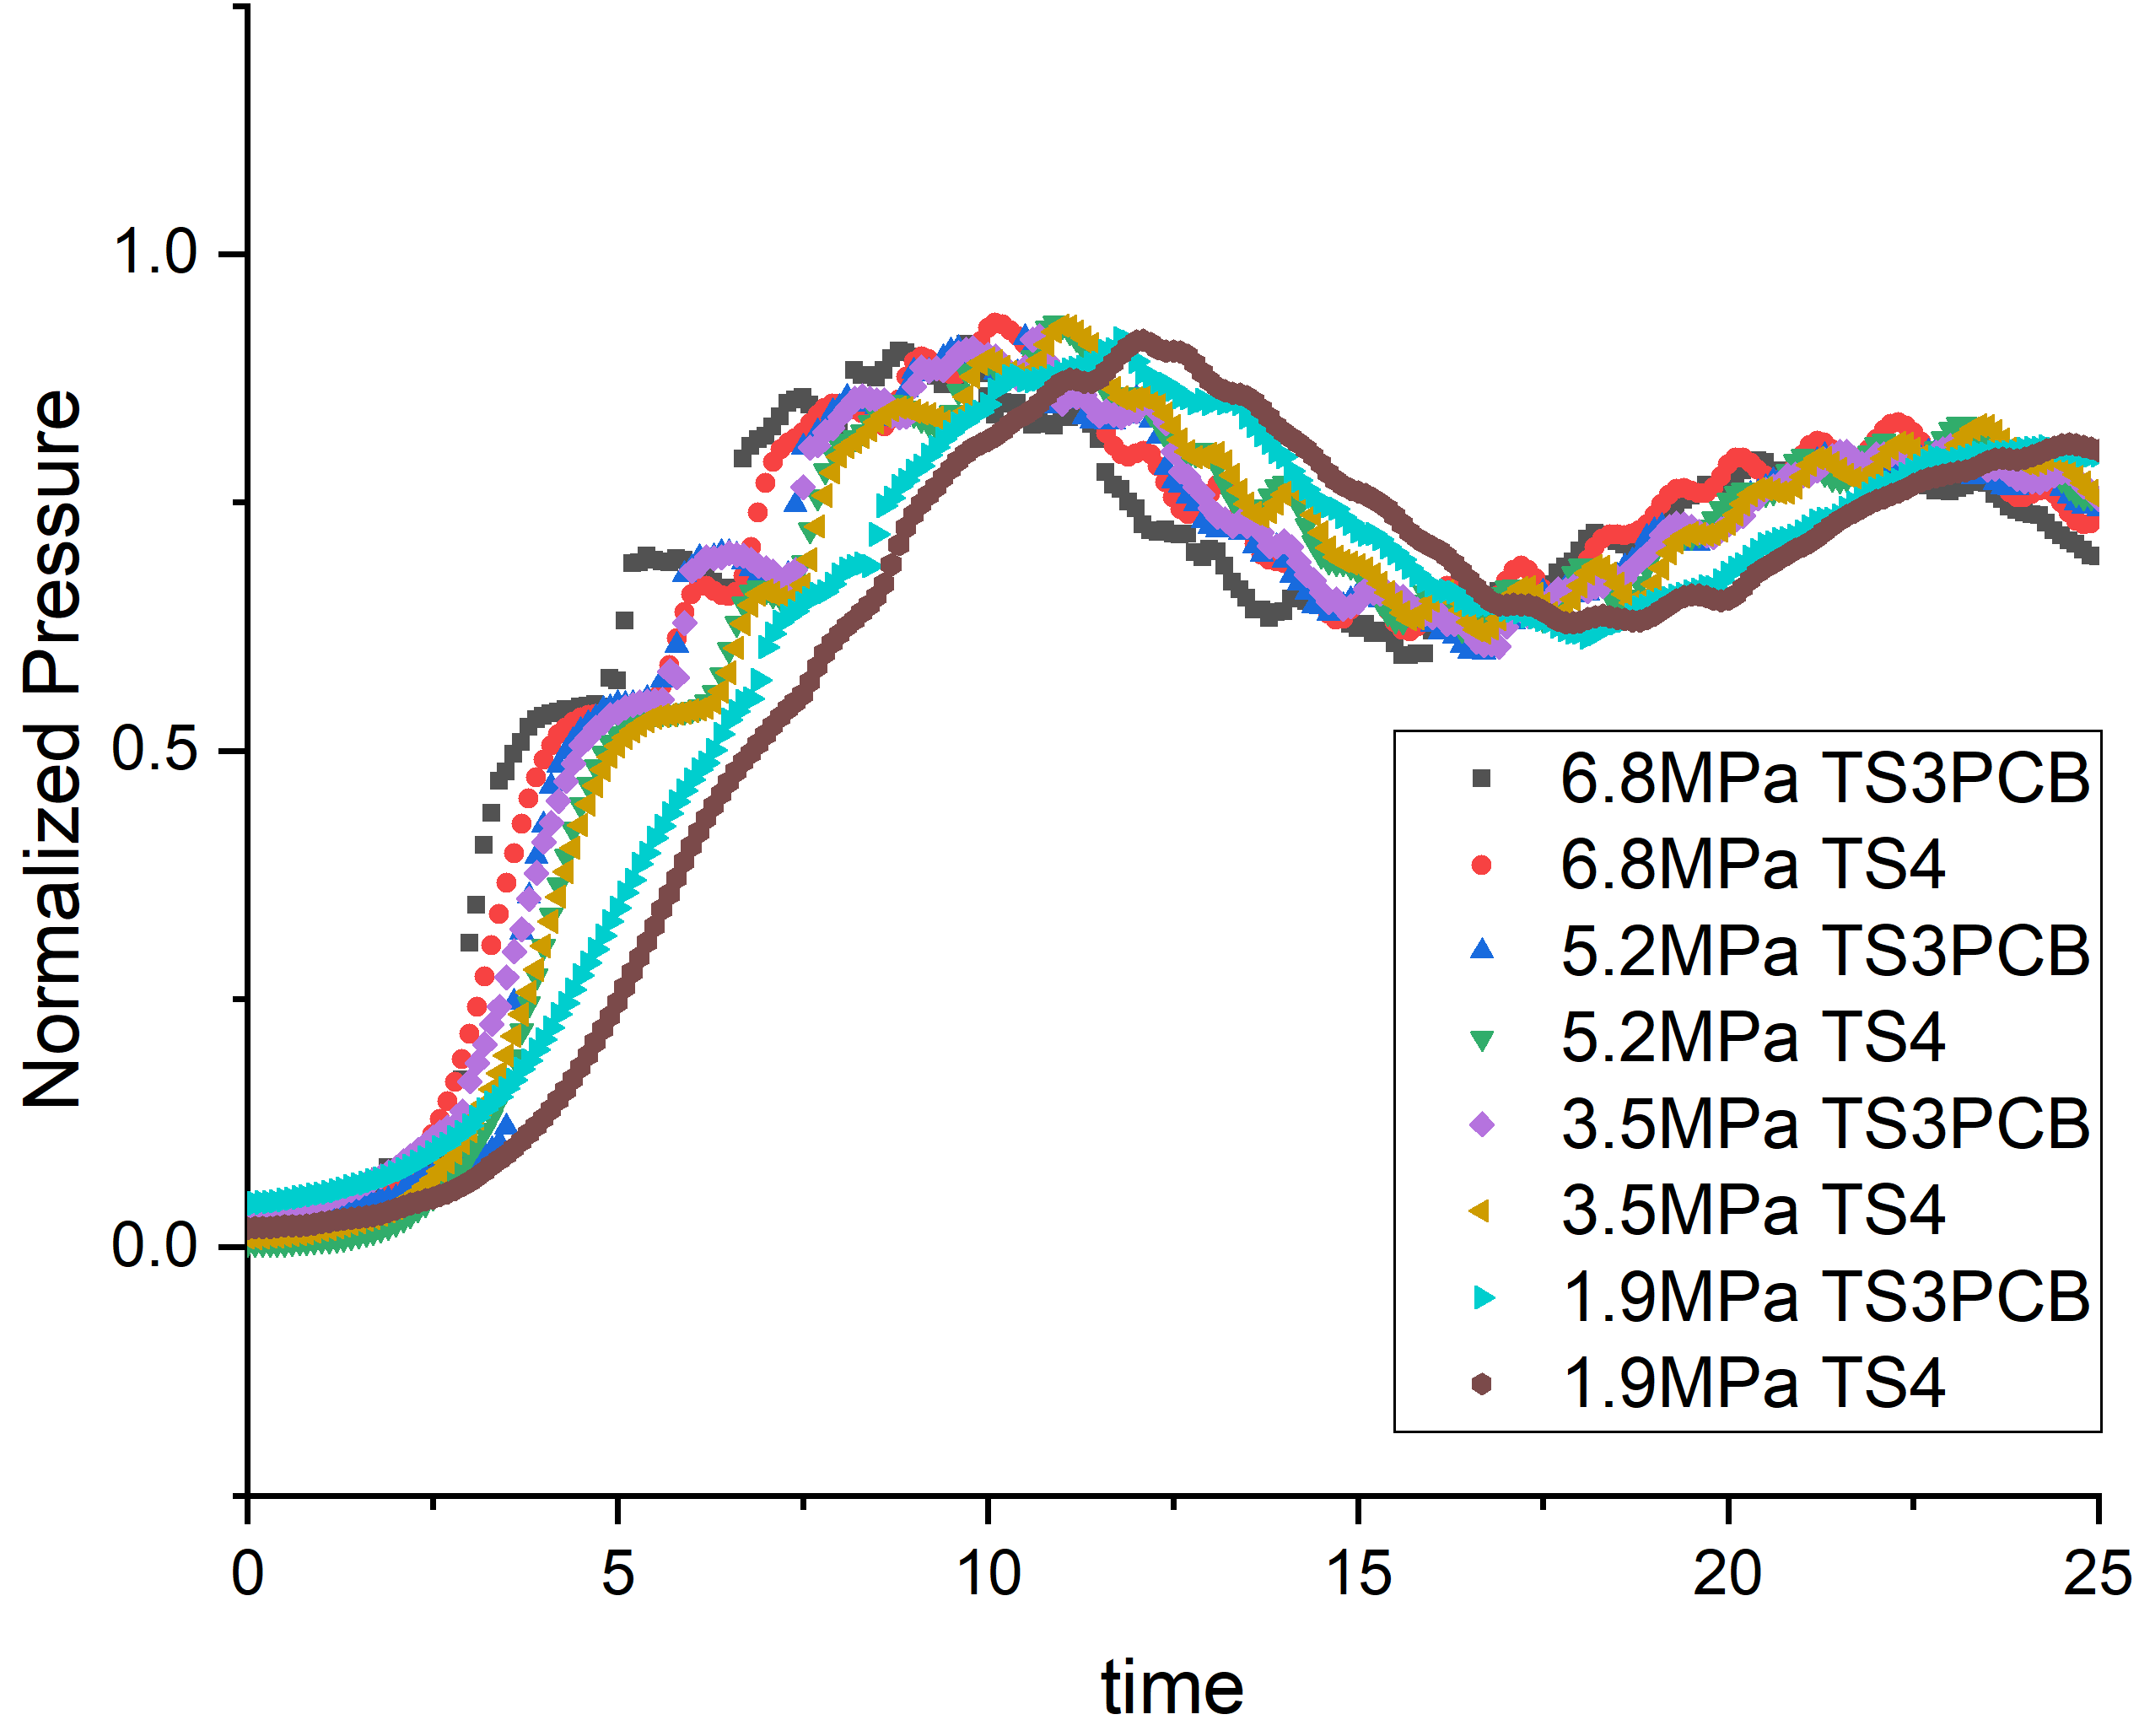
\includegraphics[width=\textwidth]{results/plots/normalized_FFKM.png}
%     \caption{Pressure evolution for four normalized tests at a selection of senors along the HENRI test section.}
%     \label{fig:piston rel}
%     \vspace{16pt}
% \end{figure}











%%%%%%%%%%%%%%%%%%%%%%%%%%%%%%%%%%%%%%%%%%%%%%%%%%%%%%%%%%%%%%%%%%%%%%%
%%%%%%%%%%%%%%%%%%%%%%%%%%%% CONCLUSION %%%%%%%%%%%%%%%%%%%%%%%%%%%%%%%
%%%%%%%%%%%%%%%%%%%%%%%%%%%%%%%%%%%%%%%%%%%%%%%%%%%%%%%%%%%%%%%%%%%%%%%
\section{Conclusions} \label{s:conclusion}
The out-of-pile HENRI prototype built at OSU is intended to provide a robust design for TREAT to implement for greater capability to simulate RIA transients for LWRs.
Previous work has proved the feasibility of the system to meet the pressurization requirements of \SI{1.72}{\mega\pascal} (\SI{250}{psi}) in \SI{5}{\milli\second} \cite{HeNURETH}.
This work presents a solution for a valve to connect the high pressure driver tank to the low pressure test section.
A valve made from a pneumatic piston, operated with the system's helium, meets the physical constraints for the HENRI system and opens fast enough to provide the desired pressurization.
The piston also provides much greater consistency over rupture disks and it can be re-used over many tests.
The durability of a metal-to-metal seal was proven to be poor, but an o-ring design with a symmetrical mount has improved the low pressure sealing ability (below \SI{1.72}{\mega\pascal} (250 psi)). The o-ring seal durability needs to be investigated and characterized further before design finalization.



%%%%%%%%%%%%%%%%%%%%%%%%%%%%%%%%%%%%%%%%%%%%%%%%%%%%%%%%%%%%%%%%%%%%%%%
%%%%%%%%%%%%%%%%%%%%%%%%% ACKNOWLEDGMENTS %%%%%%%%%%%%%%%%%%%%%%%%%%%%%
%%%%%%%%%%%%%%%%%%%%%%%%%%%%%%%%%%%%%%%%%%%%%%%%%%%%%%%%%%%%%%%%%%%%%%%
\section*{Acknowledgments}

The authors would like to acknowledge the technical and financial support for the HENRI project from the US Department of Energy- Idaho National Laboratory under the contract \# 145660-00036. The authors would also like to acknowledge the contributions of Kevin Le, Dustin Higgins, Haedon Shields, and the other members of the Marcum Research Group that have provided much support for this project.




\setlength{\baselineskip}{12pt}

\bibliographystyle{anstopical-class/nureth18new}
\bibliography{bibliography/references}

\end{document}
